\part{Part 3: Applications}

\graphicspath{ {./Pictures/} }
\chapterimage{chapter_head_2.pdf} % Chapter heading image

%++++++++++++++++++++++++++++++++++++++++++++++++++++++++++++++
\chapter{Introduction}
\label{ch:intro for tutorials}
%++++++++++++++++++++++++++++++++++++++++++++++++++++++++++++++
\section{Gmsh}
\begin{gmshnote}
	To read all about Gmsh and download its source, executables, and license please \href{http://gmsh.info}{\underline{click here}}.
\end{gmshnote}
Gmsh is an 2D/3D mesh generator including a built-in CAD engine and post-processor. Gmsh was developed to provide a fast, lightweight, and user-friendly meshing environment with additional visualization capabilities. It is open source, and the source code and executables for various operating systems (Windows, Mac, Linux) are available for free. Gmsh contains modules for geometry definition, meshing, solving and post-processing. Each module has its own set of commands and utilities, which can be easily manipulated using a graphical user-interface (GUI).

Upon launching the Gmsh executable, the GUI will open and the the module panel appears on the left-hand side of the window with headings to control the:
\begin{itemize}
    \item \textbf{Geometry}
    \item \textbf{Mesh}
    \item \textbf{Solver}
\end{itemize}
The \textbf{Geometry} section is a module that allows you to create your own geometry directly within Gmsh, or import external CAD files. Geometry in Gmsh is defined using a hierarchical structure. This means a volume is made up of different surfaces, and each surface is made up of different curves or lines. In turn, each curve or line is bounded by two end points in the case of a straight line, or a sequence of points in the case of a spline, for example. Therefore, to define a desired geometry a set of points are specified first, and the connections between these points are built using straight lines or curves. Then, a set of surfaces are created using the lines and curves, which are themselves used to define a volume in the case of a three-dimensional problem.

The geometry module has some key features to allow you to accomplish these tasks. Some of the important features are:
\begin{itemize}
    \item \textbf{Elementary entities}: Create, merge, split or delete points, lines, curves, faces or volumes.
    \item \textbf{Physical groups}: Specify boundary conditions and physical properties of a particular geometric entity.
    \item \textbf{Reload script}: Re-read the geometry saved in your .geo file, the Gmsh native file format.
    \item \textbf{Edit script}: Edit the .geo file manually using a built-in text editor.
\end{itemize}
It is worth noting that geometry specifications are saved in the .geo file in plain text format. This allows you to manually manipulate your geometry or any other specifications by editing this file using either the in-built text editor, or an external one of your choice. 

After building the geometry and defining the boundary conditions via the \textbf{Geometry} module, the next step is usually to generate a mesh of the geometry using the \textbf{Mesh} module. This module splits the geometry up into a number of simple geometric elements, such as: lines, triangles, tetrahedra, hexahedra and pyramids. Gmsh has several different algorithms for automatically generating a mesh, and an unstructured mesh will be generated by default. The \textbf{Mesh} module has sections that help to specify the type, number, and density of the mesh in the computational domain. Some of the important sections are:
\begin{itemize}
    \item \textbf{Define}: Set the number of points and stretching ratios along lines. Additionally, control the mesh type (whether structured or unstructured).
    \item \textbf{2D/3D}: Generates the mesh for surfaces/volumes in the domain. It automatically generates the mesh using specifications provided in the \textbf{Define} section.
\end{itemize}
There is another module named \textbf{Solver}, which allows a numerical solver to be accessed directly from within Gmsh. In the context of the current book, this will not be used.

\section{SU2}
\begin{su2note}
	To read all about SU2 and download its source, executables, and license please \href{https://su2code.github.io/}{\underline{click here}}.
\end{su2note}
As discussed in the Physics and Numerics parts of this book, ultimately an approximate solution to the Navier-Stokes or RANS equations is obtained by solving a discrete system of equations on a computational grid, or mesh. SU2 is an open-source CFD solver built specifically for this task. SU2 is written in C++, and its primary applications are computational aerodynamics and shape optimization. SU2 is generally user-friendly, and pre-compiled versions are available for all major operating systems (Windows, Mac, Linux). In the following tutorials we will demonstrate the utility of SU2 as a CFD tool for computational aerodynamics.

%++++++++++++++++++++++++++++++++++++++++++++++++++++++++++++++
\section{Paraview}
\begin{paraviewnote}
	To read all about Paraview and download its source, executables, and license please \href{https://www.paraview.org/}{\underline{click here}}.
\end{paraviewnote}
After SU2 runs it generates a set of data files, which includes the complete flow field solved on the mesh generated previously using Gmsh. This data must be post-processed to visualize flow structures of interest, such as the velocity or pressure fields. Paraview is an open-source and multi-platform visualization package designed for this task. It is also available for all operating systems (Windows, Mac, Linux) and is free to download and use. Paraview is designed specifically to handle large complex data sets, such as those generated in CFD simulations. In the following laboratory experiments, we will use Paraview as a post-processing tool for the analysis of the data produced by SU2. Typically, this analysis consists of contours of flow parameters, extracting line plots, slices, or pressure coefficient distributions.

%++++++++++++++++++++++++++++++++++++++++++++++++++++++++++++++
 \chapter{Inviscid NACA 0012}
\label{ch:Inviscid NACA 0012}
%++++++++++++++++++++++++++++++++++++++++++++++++++++++++++++++
\section{Required Files}
\begin{su2note}
	Use the following links to download the same version of SU2 for Windows (\href{https://users.encs.concordia.ca/~bvermeir/book/executables/windows/SU2_Windows.zip}{\underline{click here}}) or Mac (\href{https://users.encs.concordia.ca/~bvermeir/book/executables/osx/SU2_Mac.zip}{\underline{click here}}), the required configuration and mesh files (\href{https://gitlab.com/bvermeir/book-cfd/blob/master/tutorial/tut1_inviscid_naca0012/naca0012.zip}{\underline{click here}}), and the reference dataset (\href{https://gitlab.com/bvermeir/book-cfd/blob/master/tutorial/tut1_inviscid_naca0012/experimental_values.zip}{\underline{click here}}).
\end{su2note}
\begin{paraviewnote}
	Use the following links to download the same version of Paraview for Windows (\href{https://users.encs.concordia.ca/~bvermeir/book/executables/windows/ParaView-5.4.0-Qt5-OpenGL2-Windows-64bit.exe}{\underline{click here}}) or Mac (\href{https://users.encs.concordia.ca/~bvermeir/book/executables/osx/ParaView-5.4.0-Qt5-OpenGL2-MPI-OSX10.8-64bit.dmg}{\underline{click here}}).
\end{paraviewnote}

\section{Problem Description}
In this tutorial we are going to demonstrate how to simulate transonic inviscid flow around a NACA 0012 airfoil. Under the assumption of inviscid flow, the Euler equations will be used. Please note that this assumption is only reasonably valid at high Reynolds numbers and low angles of attack, since the contribution of the viscous terms in the Navier-Stokes equations is minimal in this case. The flow specifications are provided as:
\begin{itemize}
    \item Pressure = 101,325 Pa
    \item Temperature = 273 K
    \item Mach number = 0.8
    \item Angle of attack = 1.25 degree
\end{itemize}
This tutorial has two parts: Flow Solution and Post-Processing. In the first part we will explain how to manage the required files and settings in SU2, and then run the simulation. In the second part we will demonstrate how to use Paraview to visualize the data files generated in the first step using SU2.
%++++++++++++++++++++++++++++++++++++++++++++++++++++++++++++++
\section{Flow solution}
To run this simulation SU2 needs two files: a configuration file (\texttt{.cfg}) and a mesh file (\texttt{.su2}). Links to the required files and executables are provided at the start of this tutorial. The files include:
\begin{enumerate}
\item \texttt{inv\_NACA 0012.cfg}: the configuration file.
\item \texttt{mesh\_NACA 0012\_inv.su2}: the mesh file.
\end{enumerate}
The next step is to copy these two files in the directory you have save the SU2 executable, so everything is located in the same folder. Then, to run the simulation using the executable, mesh, and configuration files simply open a terminal window and enter the following commands:
\begin{table}[ht]
    \centering
    \begin{tabular}{|l|l|}
    \hline
    Windows     & \begin{tabular}{c} \$ cd "where you saved the package" \\ \$ SU2\_CFD.exe inv\_NACA0012.cfg \end{tabular}
    \\
    \hline
    Mac     & \begin{tabular}{c} \$ cd "where you saved the package" \\ \$ ./SU2\_CFD inv\_NACA0012.cfg \end{tabular}
    \\
    \hline
    \end{tabular}
\end{table}

The SU2 solver will commence solving the problem and will print out the residuals at every iteration, until the specified convergence criteria is achieved. The computational time for this case is highly dependant on the computer's performance. However, the run time is supposed to be about 15 minutes on average. After the calculations are complete the following output files should have been generated within in the SU2 folder:
\begin{itemize}
    \item \texttt{flow.vtk}: The flow solution on the entire domain.
    \item \texttt{force\_breakdown.dat}: Forces and moment on the airfoil.
    \item \texttt{history.vtk}: Convergence history.
    \item \texttt{restart\_flow.dat}: Restart file.
    \item \texttt{surface\_flow.vtk}: The flow solution on the airfoil surface.
    \item \texttt{surface\_flow.csv}: A comma separated value file of the flow solution on the airfoil.
\end{itemize}
Please keep in mind that every time you run SU2, the output data will be overwritten. Hence, before launching a new simulation you should backup your files in another directory.
%++++++++++++++++++++++++++++++++++++++++++++++++++++++++++++++
\section{Post-Processing}
In this section we will explain how to use Paraview to visualize the solution files generated by SU2. First of all, install Paraview using the links at the start of this tutorial. Once that is complete, perform the following steps to visualize the results:
%--------------------------------------------------------------
\subsection{Load the Solution File:}

\begin{enumerate}[label=\arabic*)]
    \item Launch Paraview.
    \item Go to \textbf{File} $\rightarrow$ \textbf{Open}, and then select the \texttt{flow.vtk} file. On the left-hand side of the Paraview window you will see the file appear under \textbf{builtin} in the \textbf{Pipeline Browser}.
    \item Now press the \textbf{Apply} button in the \textbf{Properties} tab, right under the \textbf{Pipeline Browser} heading. After taking these steps, your file is loaded by Paraview and is ready to be visualized (Figure \ref{fig1:load}).
\end{enumerate}
\begin{figure}[ht]
    \centering
    \includegraphics[width=0.4\textwidth]{tut01/loadvtkfile.pdf}
    \caption{Loading the \texttt{.vtk} file into the \textbf{Pipeline Browser}.}
    \label{fig1:load}
\end{figure}
%--------------------------------------------------------------
\subsection{Visualize the Mesh}
In order to view the mesh that was stored in the \texttt{.su2} file, and as shown in Figure \ref{fig1:wireframe}, select \textit{Solid Color} with \textit{Wireframe} in the toolbar. Then, you can zoom in to see the mesh near the surface of the airfoil, as shown in Figure \ref{fig1:mesh}. The mesh around the NACA 0012 is unstructured, and the elements are clustered around the leading and trailing edges to resolve the complex flow structures that are expected there.
\begin{figure}[ht]
    \centering
    \includegraphics[width=0.6\textwidth]{tut01/wireframe.pdf}
    \caption{Displaying the NACA 0012 mesh.}
    \label{fig1:wireframe}
\end{figure}
\begin{figure}[ht]
    \centering
    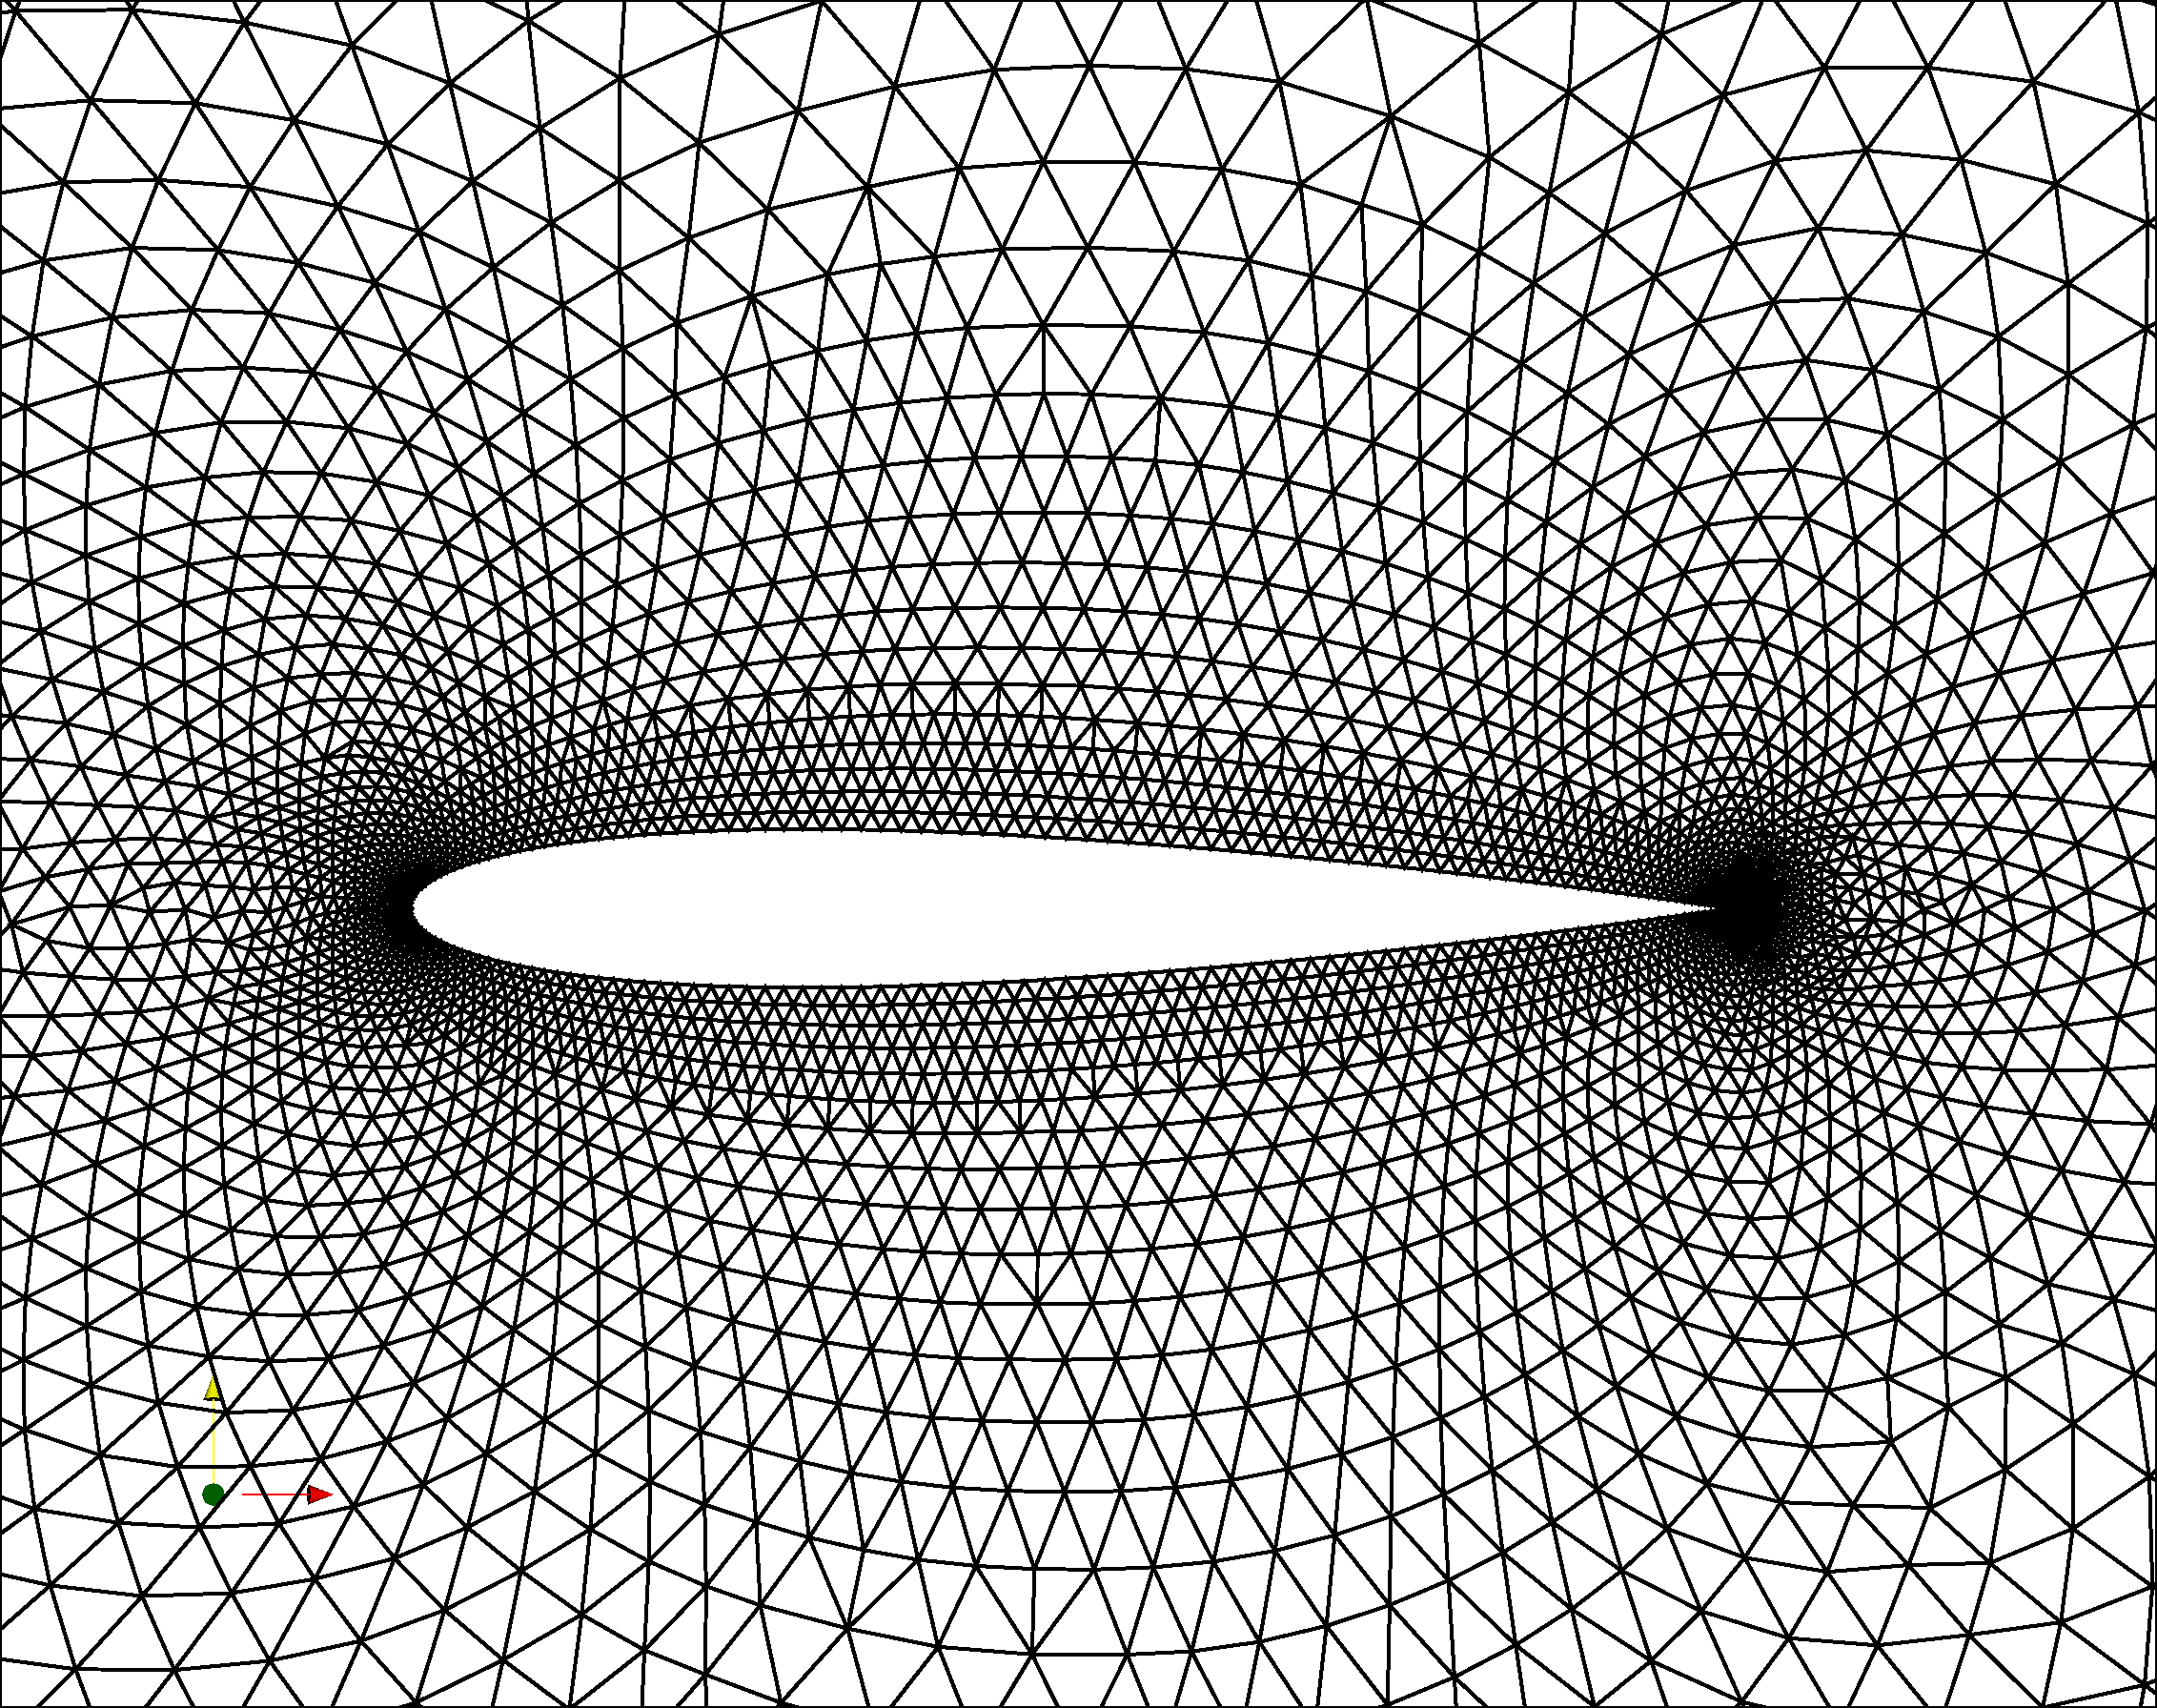
\includegraphics[width=.55\textwidth]{tut01/mesh.pdf}
    \caption{The unstructured mesh around the NACA 0012 airfoil.}
    \label{fig1:mesh}
\end{figure}
%--------------------------------------------------------------
\subsection{Visualize Pressure Contours}
In order to visualize pressure contours, you can take the following steps:
\begin{enumerate}[label=\arabic*)]
    \item Click on \texttt{flow.vtk} from within the \textbf{Pipeline Browser} to select the current data file. Then click on the \textbf{Properties} tab.
    \item According to Figure \ref{fig1:colorby}, in the \textbf{Coloring} section select \textit{Pressure} from the drop-down menu.
\end{enumerate}
\begin{figure}[H]
    \centering
    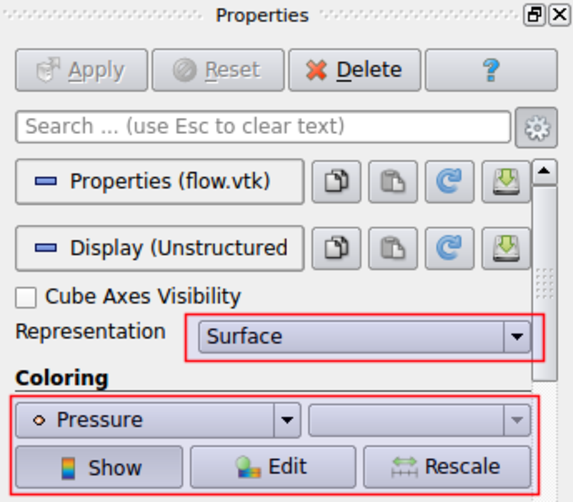
\includegraphics[width=0.4\textwidth]{tut01/contourdisplay.pdf}
    \caption{Contour settings in the \textbf{Display} tab.}
    \label{fig1:colorby}
\end{figure}
\begin{enumerate}[label=\arabic*)]
	\setcounter{enumi}{2}
    \item To change the color settings used to show the pressure field you can click on \textbf{Edit} under the \textbf{Coloring} options. Another display window appears on the right-hand side of the monitor, similar to Figure \ref{fig1:change_color_range}. Now you can change the maximum/minimum range of pressure to your desired values using the \textbf{Set Range} option, or change the contour colors using \textbf{Choose Preset} field (Figure \ref{fig1:change_color_range}). After these steps, the pressure contours shown in the display window should be similar to those shown in Figure \ref{fig1:pressure_contour}.
\end{enumerate}
\begin{figure}[!h]
    \centering
    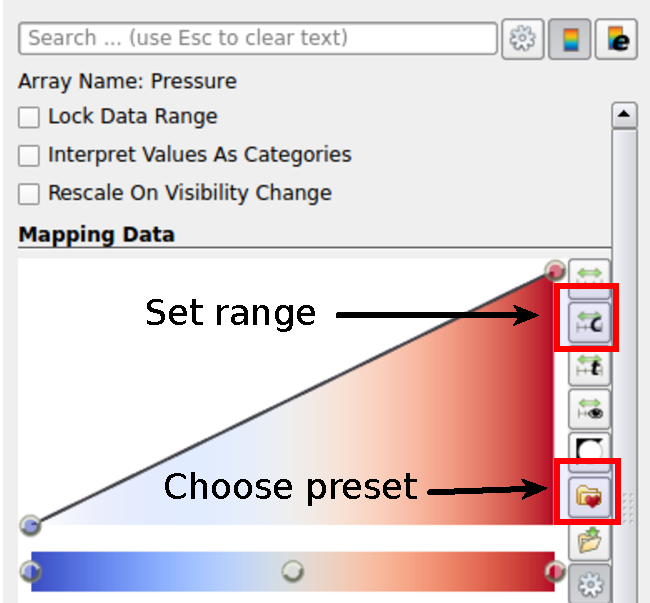
\includegraphics[width=0.4\textwidth]{tut01/colormap.pdf}
    \caption{How to change color and max/min values for contours.}
    \label{fig1:change_color_range}
\end{figure}
\begin{figure}[!h]
    \centering
    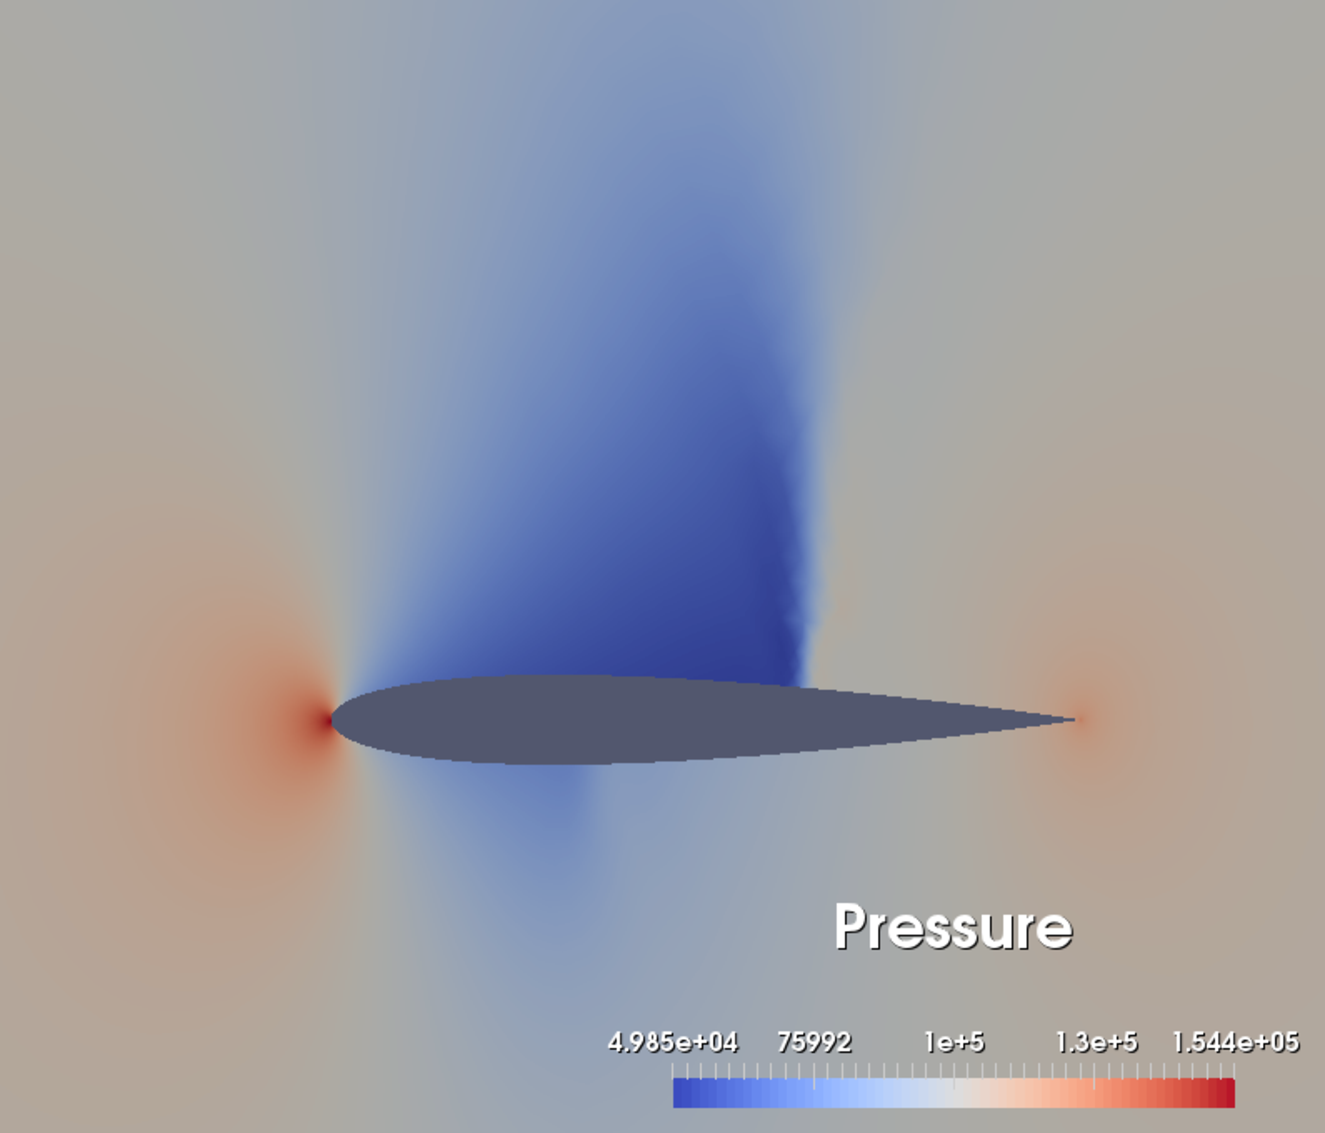
\includegraphics[width=.55\textwidth]{tut01/pressurecontour1.pdf}
    \caption{Pressure contour for NACA 0012 airfoil.}
    \label{fig1:pressure_contour}
\end{figure}
\begin{enumerate}[label=\arabic*)]
	\setcounter{enumi}{3}
	\item To add contour lines, click again on the \texttt{flow.vtk} file in the \textbf{Pipeline Browser}, and then click on the \textbf{Contour} icon (Figure \ref{fig1:contour_icon}) in the toolbar.Now you should see that a new item called \textit{Contour1} appears under \texttt{flow.vtk} in the \textbf{Pipeline Browser} (Figure \ref{fig1:contour1}).
\end{enumerate}
\begin{figure}[!h]
    \centering
    \includegraphics[width=0.5\textwidth]{tut01/contourlineicon.pdf}
    \caption{Contour icon in the toolbar.}
    \label{fig1:contour_icon}
\end{figure}
\begin{figure}[!h]
    \centering
    \includegraphics[width=0.4\textwidth]{tut01/contour1.pdf}
    \caption{Adding \textit{Contour1} in \textbf{Pipeline Browser}.}
    \label{fig1:contour1}
\end{figure}

\begin{enumerate}[label=\arabic*)]
	\setcounter{enumi}{4}
	\item Go to the \textbf{Properties} tab (as shown in Figure \ref{fig1:contourby a}), and select \textit{Pressure} from the \textbf{Contour By} drop-down menu. \item Click on the \textbf{New Range} icon to customize the range of contour lines that will be generated.
	\item For now, set the number of steps to 20, similar to Figure \ref{fig1:contourby b}. This means the pressure contour range is equally divided by 20 portions between the minimum and maximum values. Finally, click on \textbf{Apply} to generate these contour lines in the display window.
\end{enumerate}
\begin{figure}[!h]
    \centering
     \begin{subfigure}[b]{.4\textwidth}
         \centering
         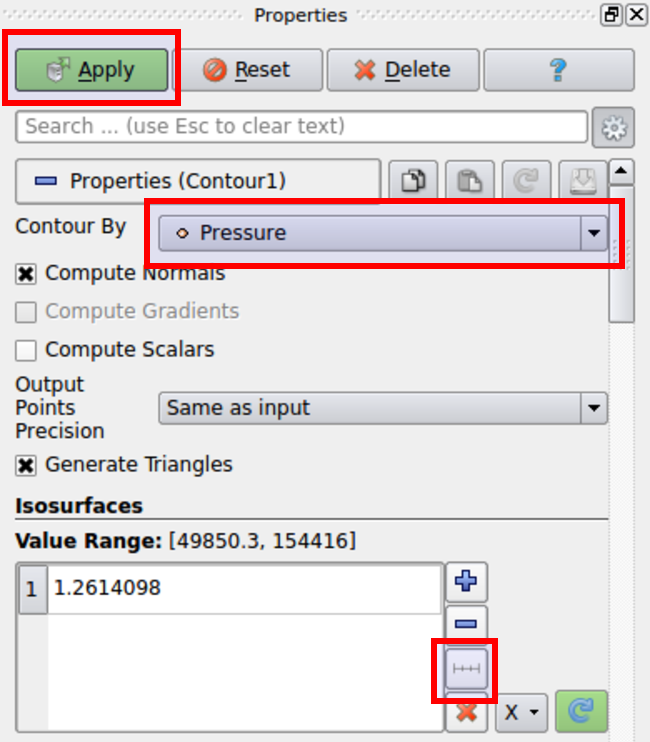
\includegraphics[width=1.0\textwidth]{tut01/contourlinenewrange.pdf}
         \caption{Define a new range}
         \label{fig1:contourby a}
     \end{subfigure}
     \hfill
     \begin{subfigure}[b]{.4\textwidth}
         \centering
         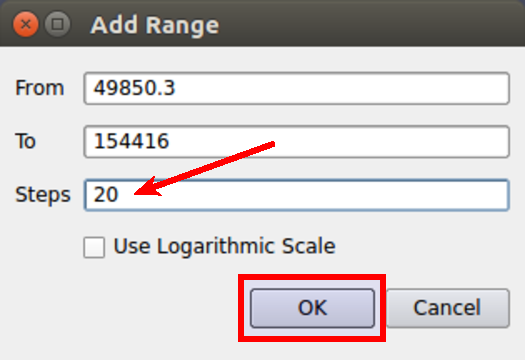
\includegraphics[width=1.0\textwidth]{tut01/addrangepdf.pdf}
         \caption{Add range}
         \label{fig1:contourby b}
     \end{subfigure}     
    \caption{How to define a new range for the contour lines.}
    \label{fig1:contourby}
\end{figure}
\begin{enumerate}[label=\arabic*)]
	\setcounter{enumi}{7}
	\item As shown in Figure \ref{fig1:colorby2}, click on \textbf{Display} under the \textbf{Properties} tab. In the \textbf{Coloring} section, select \textbf{Solid Color} from the drop-down menu, and choose white as the color using \textbf{Edit}. Now the pressure contour lines should look similar to those in Figure \ref{fig1:pressure_contour_lines}.
\end{enumerate}
\begin{figure}[!h]
    \centering
    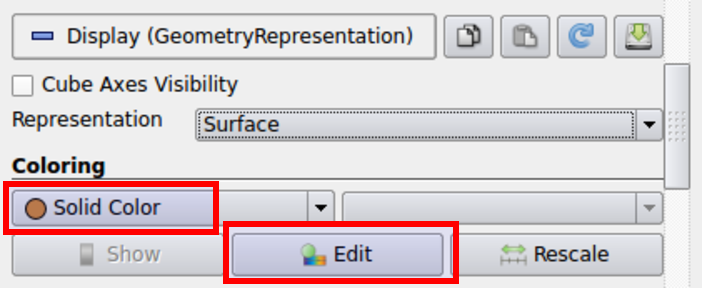
\includegraphics[width=0.5\textwidth]{tut01/coloring.pdf}
    \caption{Changing contour line colors in the \textbf{Coloring} section.}
    \label{fig1:colorby2}
\end{figure}
\begin{figure}[!h]
    \centering
    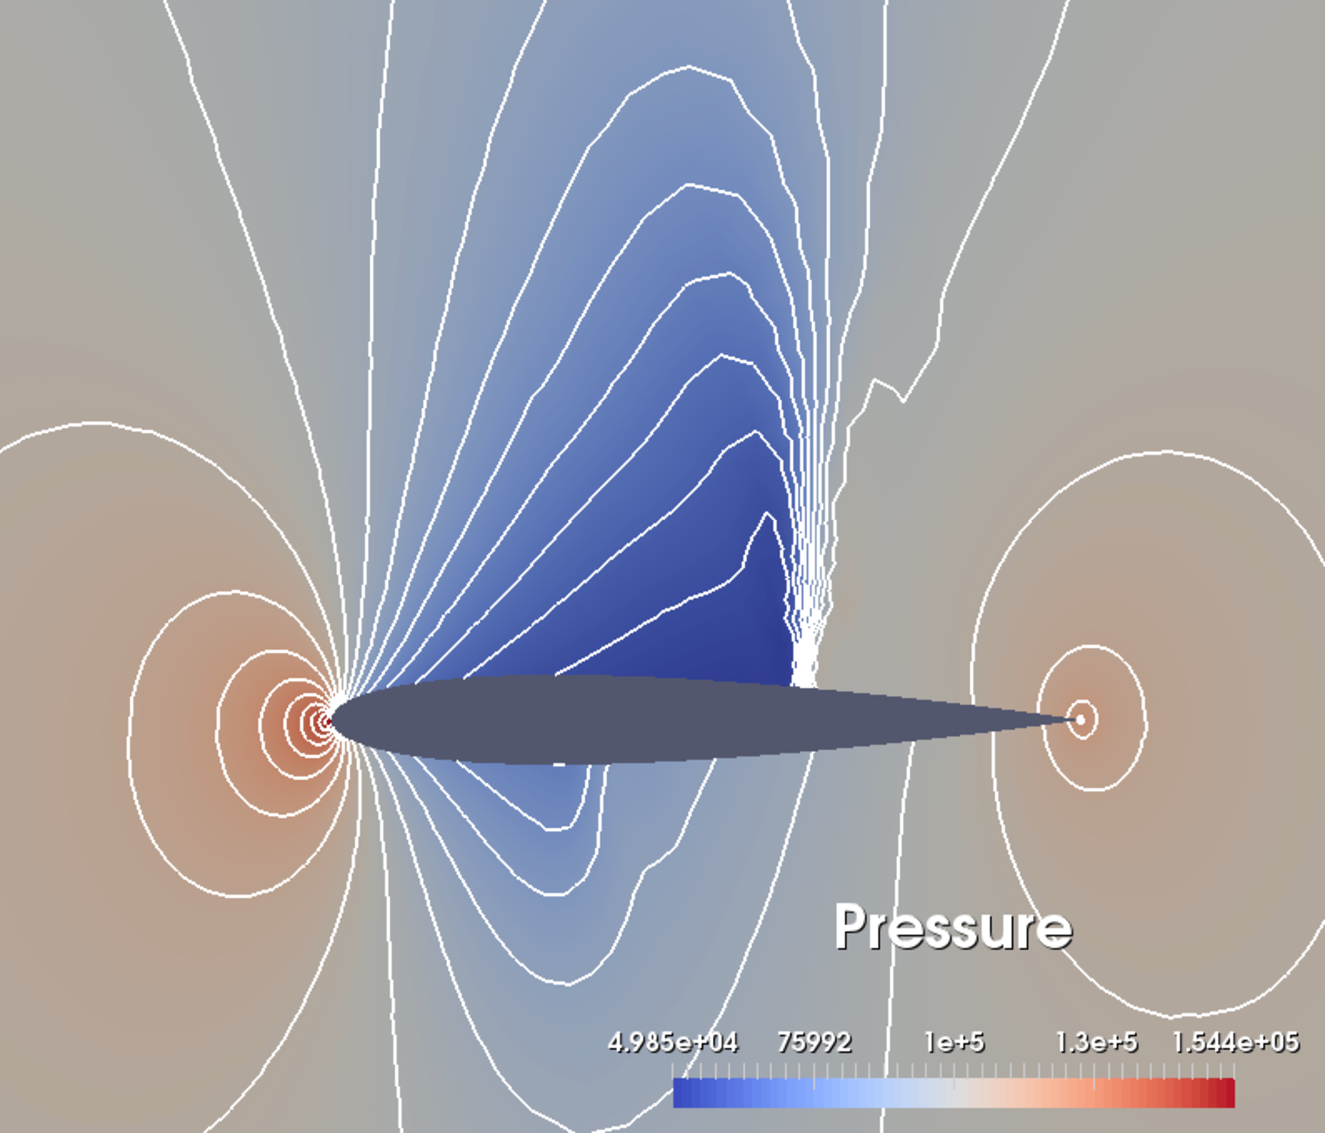
\includegraphics[width=.5\textwidth]{tut01/pressurecontour2.pdf}
    \caption{Pressure contours superimposed with contour lines around the NACA 0012 airfoil.}
    \label{fig1:pressure_contour_lines}
\end{figure}
%--------------------------------------------------------------
\subsection{Visualize the Pressure Coefficient}
The pressure data on the surface of the airfoil is stored in \texttt{surface\_flow.vtk}. We will now generate a plot of the pressure coefficient as a function of chord-wise position. To do so, you can take the following steps:
\begin{enumerate}[label=\arabic*)]
	\setcounter{enumi}{0}
	\item Go to \textbf{Open} $\rightarrow$ \textbf{File} and select \texttt{surface\_flow.vtk}. As shown in Figure \ref{fig1:builtin}, this file is now loaded and added to the list of items under \textbf{builtin} in the \textbf{Pipeline Browser}. Note that there is an eye icon on the left-hand side of each item in the \textbf{Pipeline Browser}, which enables you to hide/unhide the plots related to each item. Since we want to see only the pressure coefficient plot, we hide the previously-generated contours by unselecting the eye icon beside \texttt{flow.vtk} and \textit{Contour1}.
\end{enumerate}
\begin{figure}[!h]
    \centering
    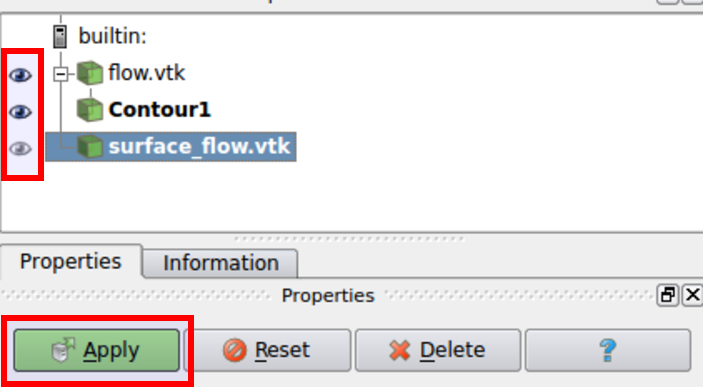
\includegraphics[width=0.4\textwidth]{tut01/eyeiconsurfaceflow.pdf}
    \caption{Loading the surface \texttt{.vtk} file into Paraview.}
    \label{fig1:builtin}
\end{figure}
\begin{enumerate}[label=\arabic*)]
	\setcounter{enumi}{1}
	\item Select \texttt{surface\_flow.vtk} in the \textbf{Pipeline Browser} (as shown in Figure \ref{fig1:plotdata}). Then, go to \textbf{Filters} $\rightarrow$ \textbf{Search} (Figure \ref{fig1:plotdata a}) and search for \textbf{Plot Data} (Figure \ref{fig1:plotdata b}). After taking this step, as shown in Figure \ref{fig1:plotdata-list}, the \textit{PlotData1} item is added to the \textbf{Pipeline Browser}.
\end{enumerate}
\begin{figure}[ht]
    \centering
     \begin{subfigure}[b]{.4\textwidth}
         \centering
         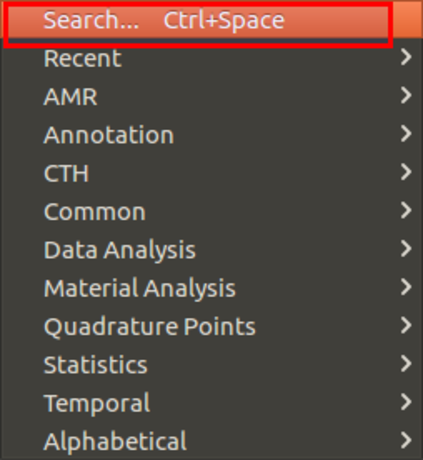
\includegraphics[width=.7\textwidth]{tut01/filtersearch.pdf}
         \caption{Searching for a \textbf{Filter}}
         \label{fig1:plotdata a}
     \end{subfigure}
     \hfill
     \begin{subfigure}[b]{.4\textwidth}
         \centering
         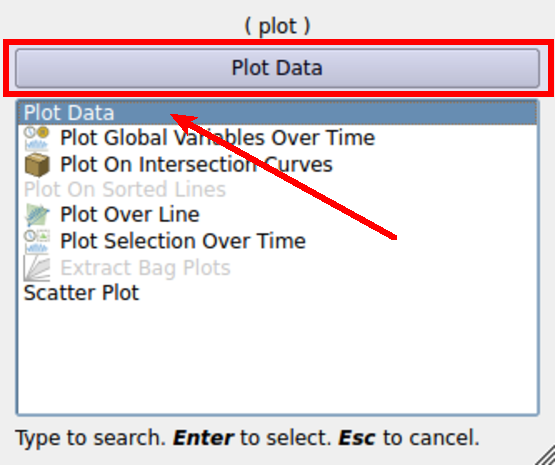
\includegraphics[width=.9\textwidth]{tut01/plotdatasearch.pdf}
         \caption{Searching for the \textbf{PlotData} filter}
         \label{fig1:plotdata b}
     \end{subfigure}     
    \caption{How to plot data.}
    \label{fig1:plotdata}
\end{figure}
\begin{enumerate}[label=\arabic*)]
	\setcounter{enumi}{2}
	\item Hide (deactivate) all items in the list of the \textbf{Pipeline Browser} except \textit{PlotData1} by clicking on the eye icons beside each, and then click on \textbf{Apply}.
	\item As shown in Figure \ref{fig1:pointsx}, under \textbf{Display} in the \textbf{Properties} tab deactivate \textbf{Use Index For XAxis}, and then select \textit{Points\_X} from the drop-down menu.
	\item Under \textbf{Series Parameters} in the same tab, unselect all variables except for \textit{Pressure\_Coefficient}. This allows you to have only one plot showing the pressure coefficient versus chord wise position. The pressure plot in the display window should be similar to that shown in Figure \ref{fig1:surface_pressure}.
\end{enumerate}
\begin{figure}[ht]
    \centering
    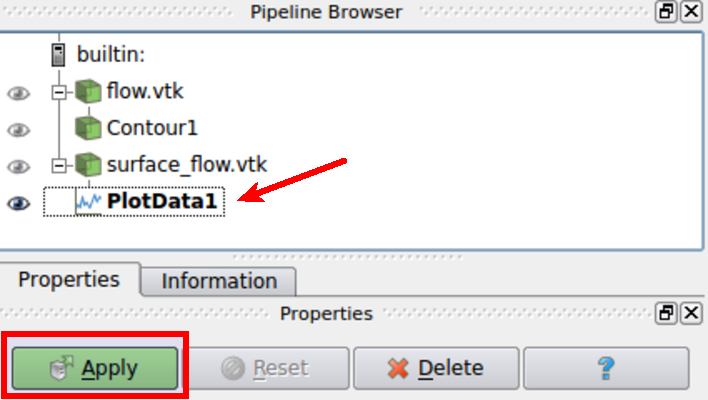
\includegraphics[width=0.45\textwidth]{tut01/plotdata1.pdf}
    \caption{Adding \textit{PlotData1} to the \textbf{Pipeline Browser}.}
    \label{fig1:plotdata-list}
\end{figure}
\begin{figure}[H]
    \centering
    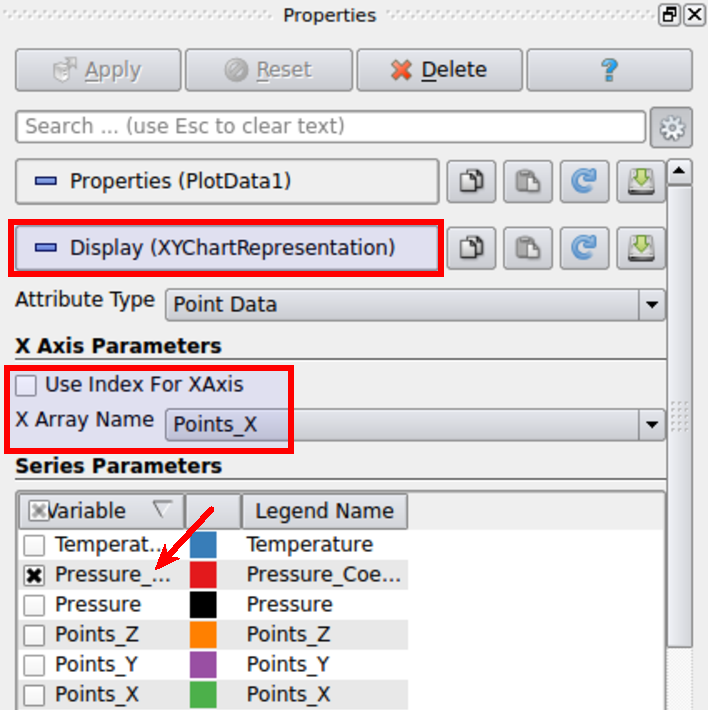
\includegraphics[width=0.4\textwidth]{tut01/plotcurvesetting.pdf}
    \caption{Plot settings for pressure coefficient along the airfoil surface.}
    \label{fig1:pointsx}
\end{figure}
\begin{figure}[ht]
    \centering
    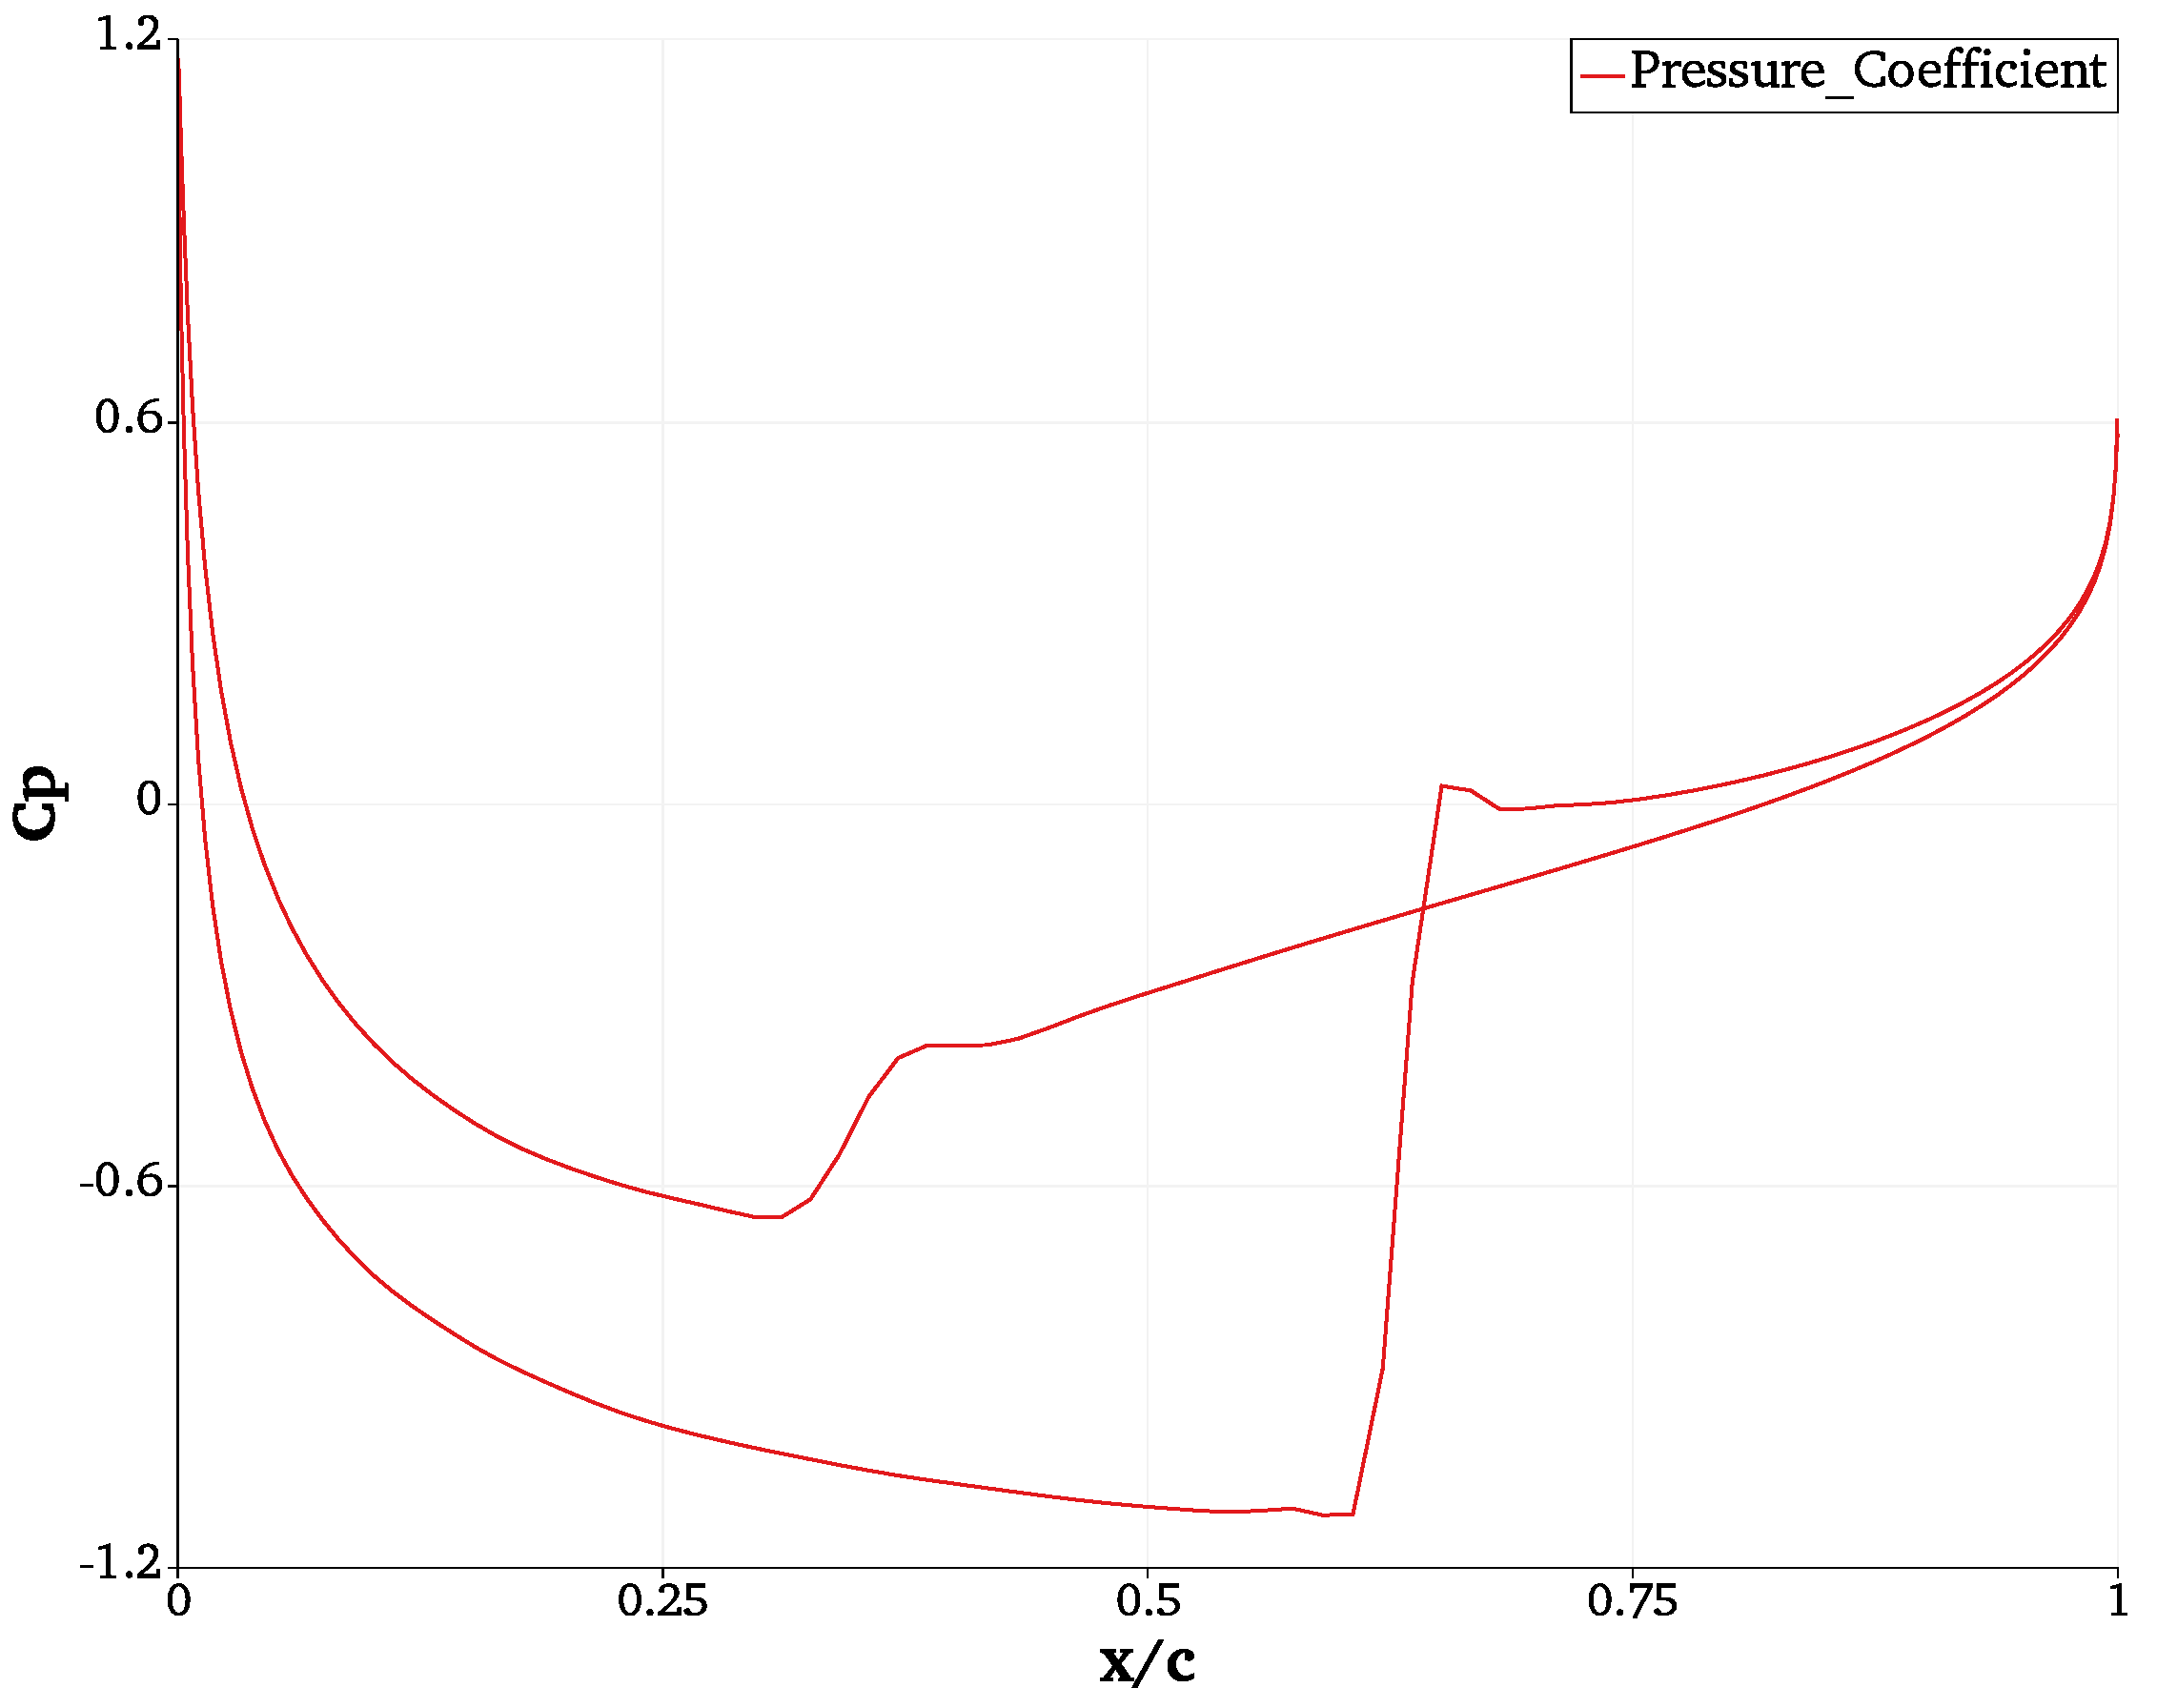
\includegraphics[width=.75\textwidth]{tut01/plot11.pdf}
    \caption{Pressure coefficient on the surface of the NACA 0012 airfoil.}
    \label{fig1:surface_pressure}
\end{figure}
By convention, $-C_p$ is typically plotted such that the pressure curve on suction side (lower pressure) is on top of the pressure curve on the pressure side (higher pressure). Therefore, we need to reverse the $y$-axis in this plot to flip it. To do this, you can take the following steps:
\begin{enumerate}[label=\arabic*)]
	\setcounter{enumi}{0}
	\item Go to \textbf{Display} in the \textbf{Properties} tab.
	\item Find the \textbf{Left Axis Range} section in the same tab, and then click on \textbf{Left Axis Use Custom Range} (Figure \ref{fig1:viewsetting}). 
	\item Later, another section appears to select maximum/minimum ranges for the left axis of the plot. Now, switch numbers in these two text bars. This allows the $y$-axis to be reverse (flipped).
	\item There are other parameters that you may want to change in the same tab, such as the \textbf{Left Axis Title} or the \textbf{Bottom Axis Title}. Please type $C_p$ and $x/c$ in \textbf{Left Axis Title} and \textbf{Bottom Axis Title}, respectively.
	\item For adding markers to the plot lines, from \textbf{Display} select the \textbf{Marker Style} as \textit{Diamond} (Figure \ref{fig1:marker}). You can also change the thickness of the plot line in the same tab.
\end{enumerate}
After taking all these steps, the final plot you get should be similar to Figure \ref{fig1:surface_pressure2}.
\begin{figure}[ht]
    \centering
    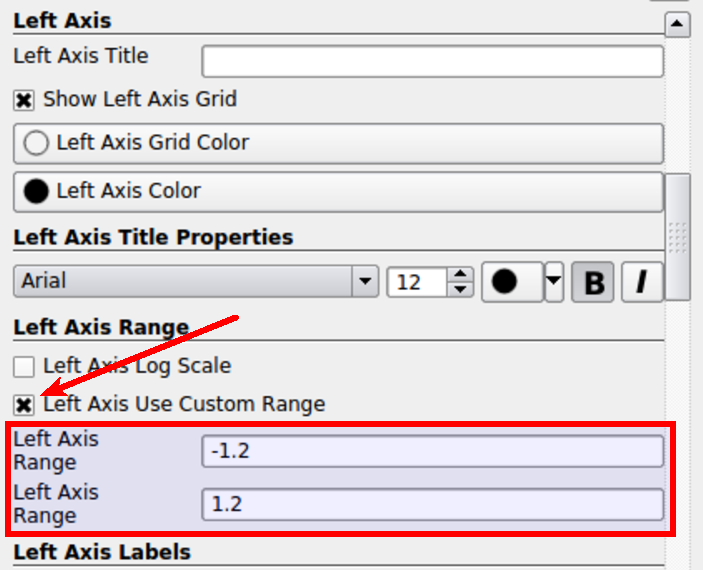
\includegraphics[width=0.4\textwidth]{tut01/leftaxis.pdf}
    \caption{Plot Settings.}
    \label{fig1:viewsetting}
\end{figure}
\begin{figure}[H]
    \centering
    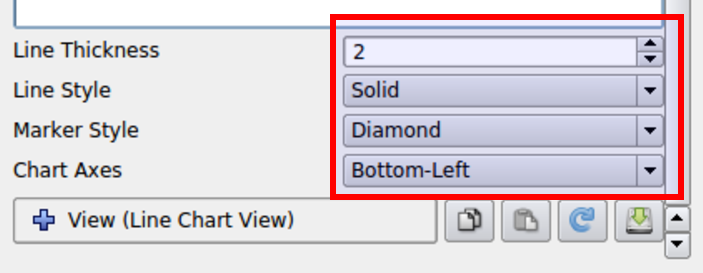
\includegraphics[width=0.4\textwidth]{tut01/addingmarker.pdf}
    \caption{How to add markers to a line plot.}
    \label{fig1:marker}
\end{figure}

\begin{figure}[ht]
    \centering
    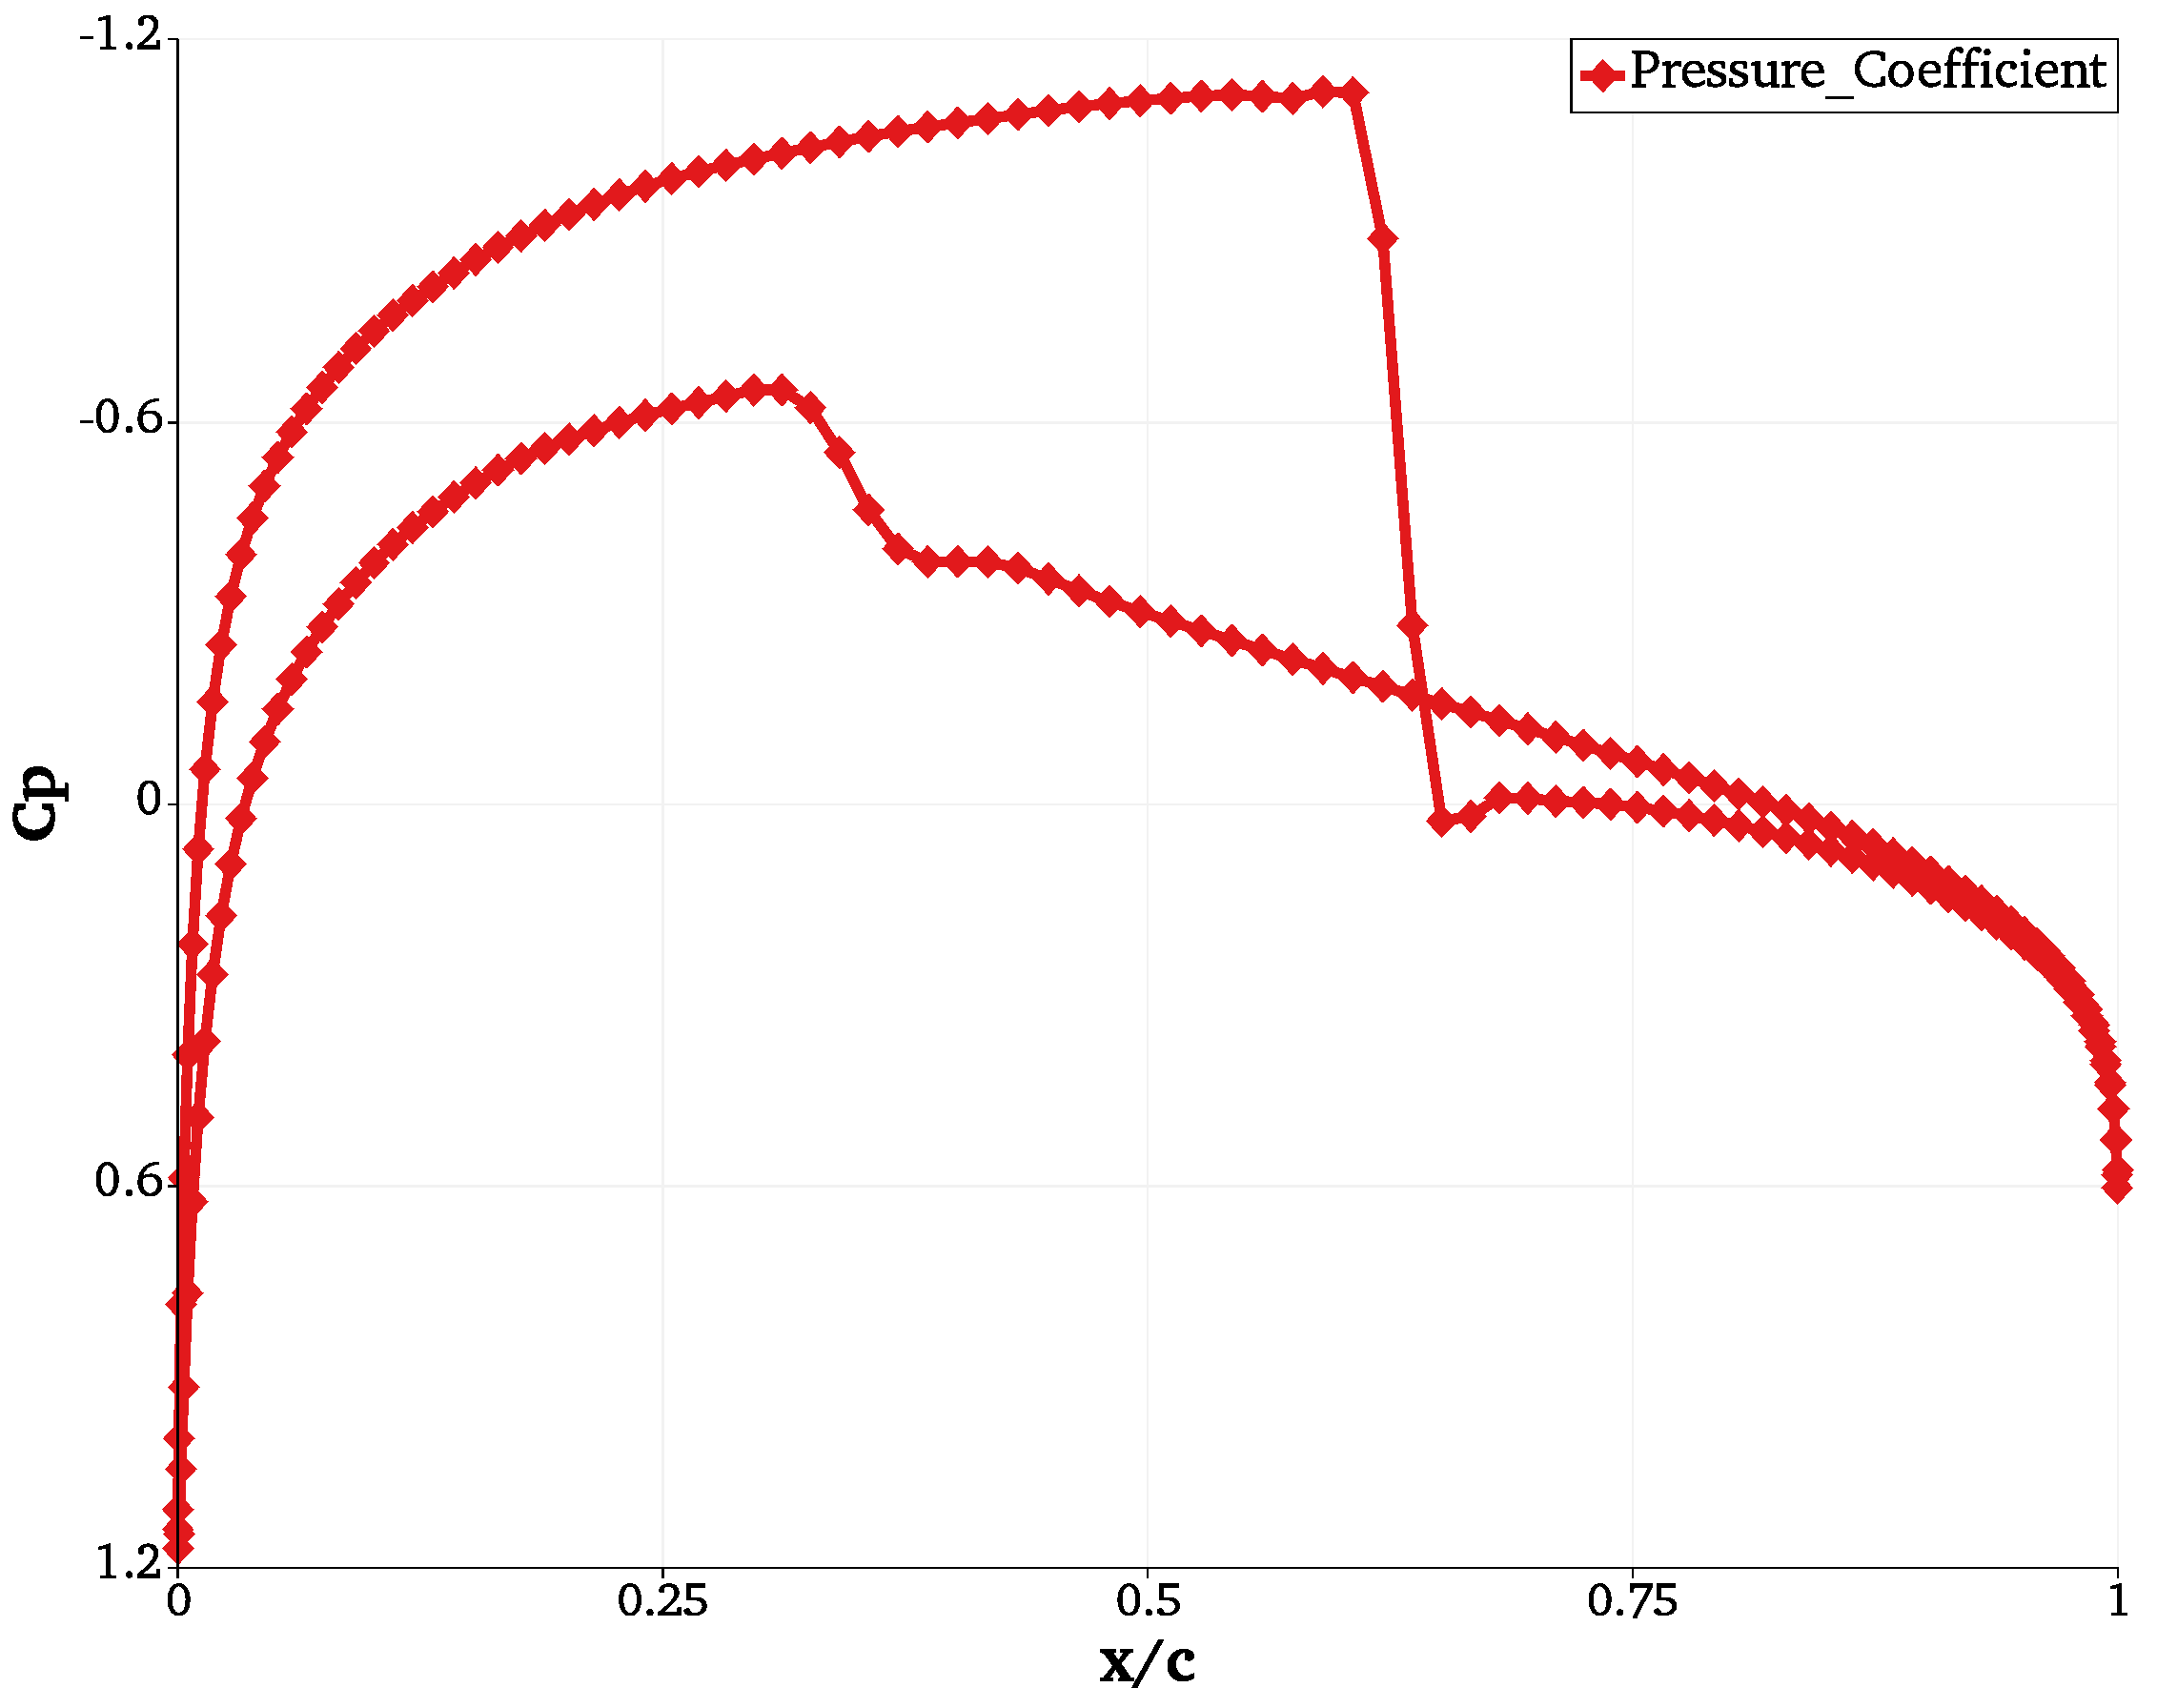
\includegraphics[width=.65\textwidth]{tut01/plot22.pdf}
    \caption{Final pressure coefficient plot on the surface of the NACA 0012 airfoil.}
    \label{fig1:surface_pressure2}
\end{figure}
%--------------------------------------------------------------
\subsection{Aerodynamic Forces}
In order to obtain the aerodynamic forces on the airfoil open \texttt{force\_breakdown.dat} using a text editor. As shown in Figure \ref{fig1:forcefile1}, the flow properties are tabulated and it can be confirmed that they agree with the configuration file. 
\begin{figure}[ht]
    \centering
    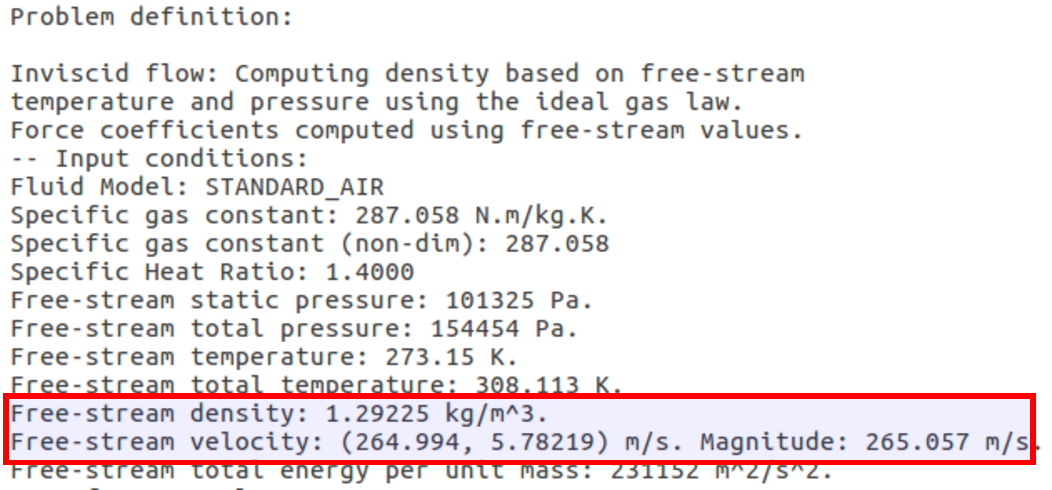
\includegraphics[width=0.7\textwidth]{tut01/forcefile1.pdf}
    \caption{Fluid and flow properties in \texttt{force\_breakdown.dat}.}
    \label{fig1:forcefile1}
\end{figure}

As shown in Figure \ref{fig1:forcefile2}, the aerodynamic forces are expressed in non-dimensional form by using free-stream values for density and velocity, as well as a unit reference length in this case. The actual dimensional forces can be obtained by multiplying the flow coefficients with these non-dimensional factors calculated with the free-stream density and velocity. Note that you can find the lift coefficient ($C_L$), drag coefficient ($C_D$), lift to drag ratio ($C_L / C_D$), the moment coefficient ($C_{M,z}$), $x$-component of force coefficient ($C_{F,x}$) and $y$-component of force coefficient ($C_{F,y}$) all from the \texttt{force\_breakdown.dat} file.
\begin{figure}[H]
	\centering
	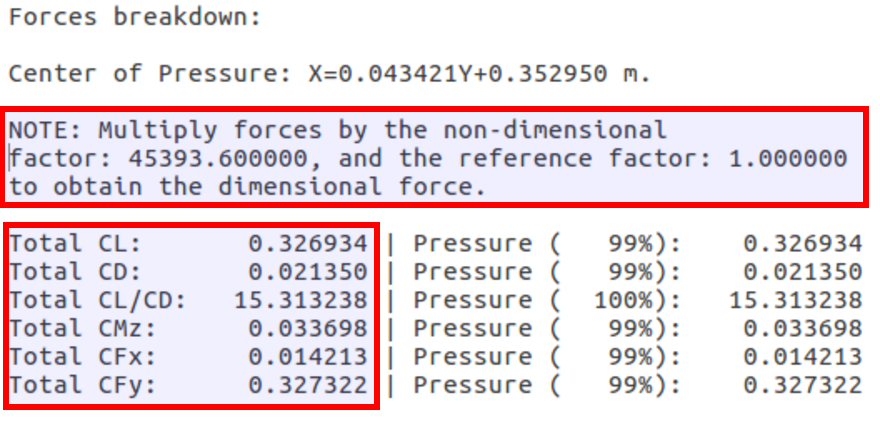
\includegraphics[width=0.6\textwidth]{tut01/forcefile2.pdf}
	\caption{Aerodynamic forces obtained from \texttt{force\_breakdown.dat}.}
	\label{fig1:forcefile2}
\end{figure}
%++++++++++++++++++++++++++++++++++++++++++++++++++++++++++++++
\section{Questions}
1. Run the provided default NACA 0012 test case at $Ma=0.8$.
\begin{enumerate}[label=(\alph*)]
    \item Plot and comment on the mesh.
    \item Plot and comment on the pressure contours around the airfoil.
    \item Plot and comment on the pressure coefficient on the surface of the airfoil.
\end{enumerate}
2. Re-run the default NACA 0012 case but change the Mach number to $Ma=0.3$, and run several simulations using $\alpha = 0, 2, 4, 6, 8, 10, 12, 14, 16$ degrees.
\begin{enumerate}[label=(\alph*)]
    \item Plot $C_{L}$ vs $\alpha$ alongside the provided experimental data provided at the start of this tutorial~\cite{ladson1988effects}.
    \item Repeat 1.b with $Ma = 0.3$ for the $\alpha = 0, 8, 16$ degree cases.
    \item Repeat 1.c with for the $\alpha = 0, 8, 16$ degree cases, and include the provided experimental data from \cite{ladson1987pressure}.
\end{enumerate}
3. Compare your CFD results in Q.2, and discuss sources of error that could have led to any discrepancies in your results relative to the experimental data.
%--------------------------------------------------------------
%++++++++++++++++++++++++++++++++++++++++++++++++++++++++++++++
%++++++++++++++++++++++++++++++++++++++++++++++++++++++++++++++
%++++++++++++++++++++++++++++++++++++++++++++++++++++++++++++++
\chapter{Supersonic Wedge}
\label{ch:Supersonic Wedge}
%++++++++++++++++++++++++++++++++++++++++++++++++++++++++++++++
\section{Required Files}
\begin{su2note}
	Use the following links to download the same version of SU2 for Windows (\href{https://users.encs.concordia.ca/~bvermeir/book/executables/windows/SU2_Windows.zip}{\underline{click here}}) or Mac (\href{https://users.encs.concordia.ca/~bvermeir/book/executables/osx/SU2_Mac.zip}{\underline{click here}}), and the required configuration and mesh files (\href{https://gitlab.com/bvermeir/book-cfd/blob/master/tutorial/tut2_supersonic_wedge/wedge.zip}{\underline{click here}}).
\end{su2note}
\begin{paraviewnote}
	Use the following links to download the same version of Paraview for Windows (\href{https://users.encs.concordia.ca/~bvermeir/book/executables/windows/ParaView-5.4.0-Qt5-OpenGL2-Windows-64bit.exe}{\underline{click here}}) or Mac (\href{https://users.encs.concordia.ca/~bvermeir/book/executables/osx/ParaView-5.4.0-Qt5-OpenGL2-MPI-OSX10.8-64bit.dmg}{\underline{click here}}).
\end{paraviewnote}

\section{Problem Description}
In this tutorial we are going to demonstrate how to simulate supersonic inviscid flow past a simple 2D wedge. This wedge generates an oblique-shock wave moving outwards from its surface. Assuming the Reynolds number is high, and that the fluid is an ideal gas, we will be using the Euler equations. The domain is approximated using a structured mesh with 3,750 nodes. The domain consists of a flat upper wall, and a lower wall with an inclined a wedge starting at $x/L=1/3$, where $L$ is the length of duct. The wedge angle is taken to be 10 degrees, and the inlet flow paramaters are:
\begin{itemize}
    \item Pressure = 101,325 Pa
    \item Temperature = 273.15 K
    \item Mach number = 2.0
    \item Wedge angle = 10 degrees
\end{itemize}
This tutorial has two parts: Flow Solution and Post-processing. In the first part, we will explain how to manage the prerequisite files and settings, and how to run the CFD simulation using SU2. In the second part we explain how to use Paraview to visualize the data obtained from SU2.
%++++++++++++++++++++++++++++++++++++++++++++++++++++++++++++++
\section{Flow solution}
To run this simulation SU2 needs two files: a configuration file (\texttt{.cfg}) and a mesh file (\texttt{.su2}). Links to the required files and executables are provided at the start of this tutorial. The files include:
\begin{enumerate}
    \item \texttt{inv\_wedge\_HLLC.cfg} which is a configuration file.
    \item \texttt{mesh\_wedge\_inv.su2} which is a a mesh file.
\end{enumerate}
The next step is to copy these two files into the same directory as the SU2 executable. Then, to run the simulation open a terminal window and enter the following commands:
\begin{table}[ht]
    \centering
    \begin{tabular}{|l|l|}
    \hline
    Windows     & \begin{tabular}{c} \$ cd "where you saved the package" \\ \$ SU2\_CFD.exe inv\_wedge\_HLLC.cfg \end{tabular}
    \\
    \hline
    Mac     & \begin{tabular}{c} \$ cd "where you saved the package" \\ \$ ./SU2\_CFD inv\_wedge\_HLLC.cfg \end{tabular}
    \\
    \hline
    \end{tabular}
\end{table}

The SU2 solver will commence solving the problem and will print out the residuals at every iteration, until the specified convergence criteria is achieved. The computational time for this case is highly dependant on the computer's performance. However, the run time is supposed to be about 15 minutes on average. After the calculations are complete the following output files should have been generated within in the SU2 folder:
\begin{itemize}
    \item \texttt{flow.vtk}: The flow solution on the entire domain.
    \item \texttt{history.vtk}: Convergence history.
    \item \texttt{restart\_flow.dat}: Restart file.
    \item \texttt{surface\_flow.vtk}: The flow solution on the airfoil surface.
\end{itemize}
Please keep in mind that every time you run SU2, the output data will be overwritten. Hence, before launching a new simulation you should backup your files in another directory.
%++++++++++++++++++++++++++++++++++++++++++++++++++++++++++++++
\section{Post-Processing}
In this section, we explain how to use Paraview to visualize the solution generated by SU2. First of all, install paraview (if not already done) using the links at the start of this tutorial. Once that is complete, perform the following steps to visualize the results:
%--------------------------------------------------------------
\subsection{Load the Solution File:}
\begin{enumerate}[label=\arabic*)]
	\item Launch Paraview.
	\item Go to \textbf{File} $\rightarrow$ \textbf{Open}, and then select the \texttt{flow.vtk} file. On the left side of the Paraview window you will see the file appears in the \textbf{Pipeline Browser} under \textbf{builtin}
	\item Now press the \textbf{Apply} button in the \textbf{Properties} tab, right under the \textbf{Pipeline Browser} heading. After taking these steps, your file is loaded by Paraview and is ready to be visualized (Figure \ref{fig2:load}).
\end{enumerate}
\begin{figure}[ht]
    \centering
    \includegraphics[width=0.4\textwidth]{tut02/loadvtkfile.pdf}
    \caption{Loading the \texttt{.vtk} file into the \textbf{Pipeline Browser}.}
    \label{fig2:load}
\end{figure}
%--------------------------------------------------------------
\subsection{Visualize the Mesh}
As shown in Figure \ref{fig2:wireframe}, in order to view the mesh select \textit{Solid Color} with \textit{Wireframe} in the toolbar. Then, you can zoom in to see the mesh for the computational domain, as shown in Figure \ref{fig2:mesh}. As you can see, the mesh in the duct is structured, and the wedge abruptly changes the direction of mesh on the bottom surface. Additionally, the grids are approximately uniform throughout the domain.
\begin{figure}[ht]
    \centering
    \includegraphics[width=0.6\textwidth]{tut02/wireframe.pdf}
    \caption{How to display the mesh.}
    \label{fig2:wireframe}
\end{figure}
\begin{figure}[ht]
    \centering
    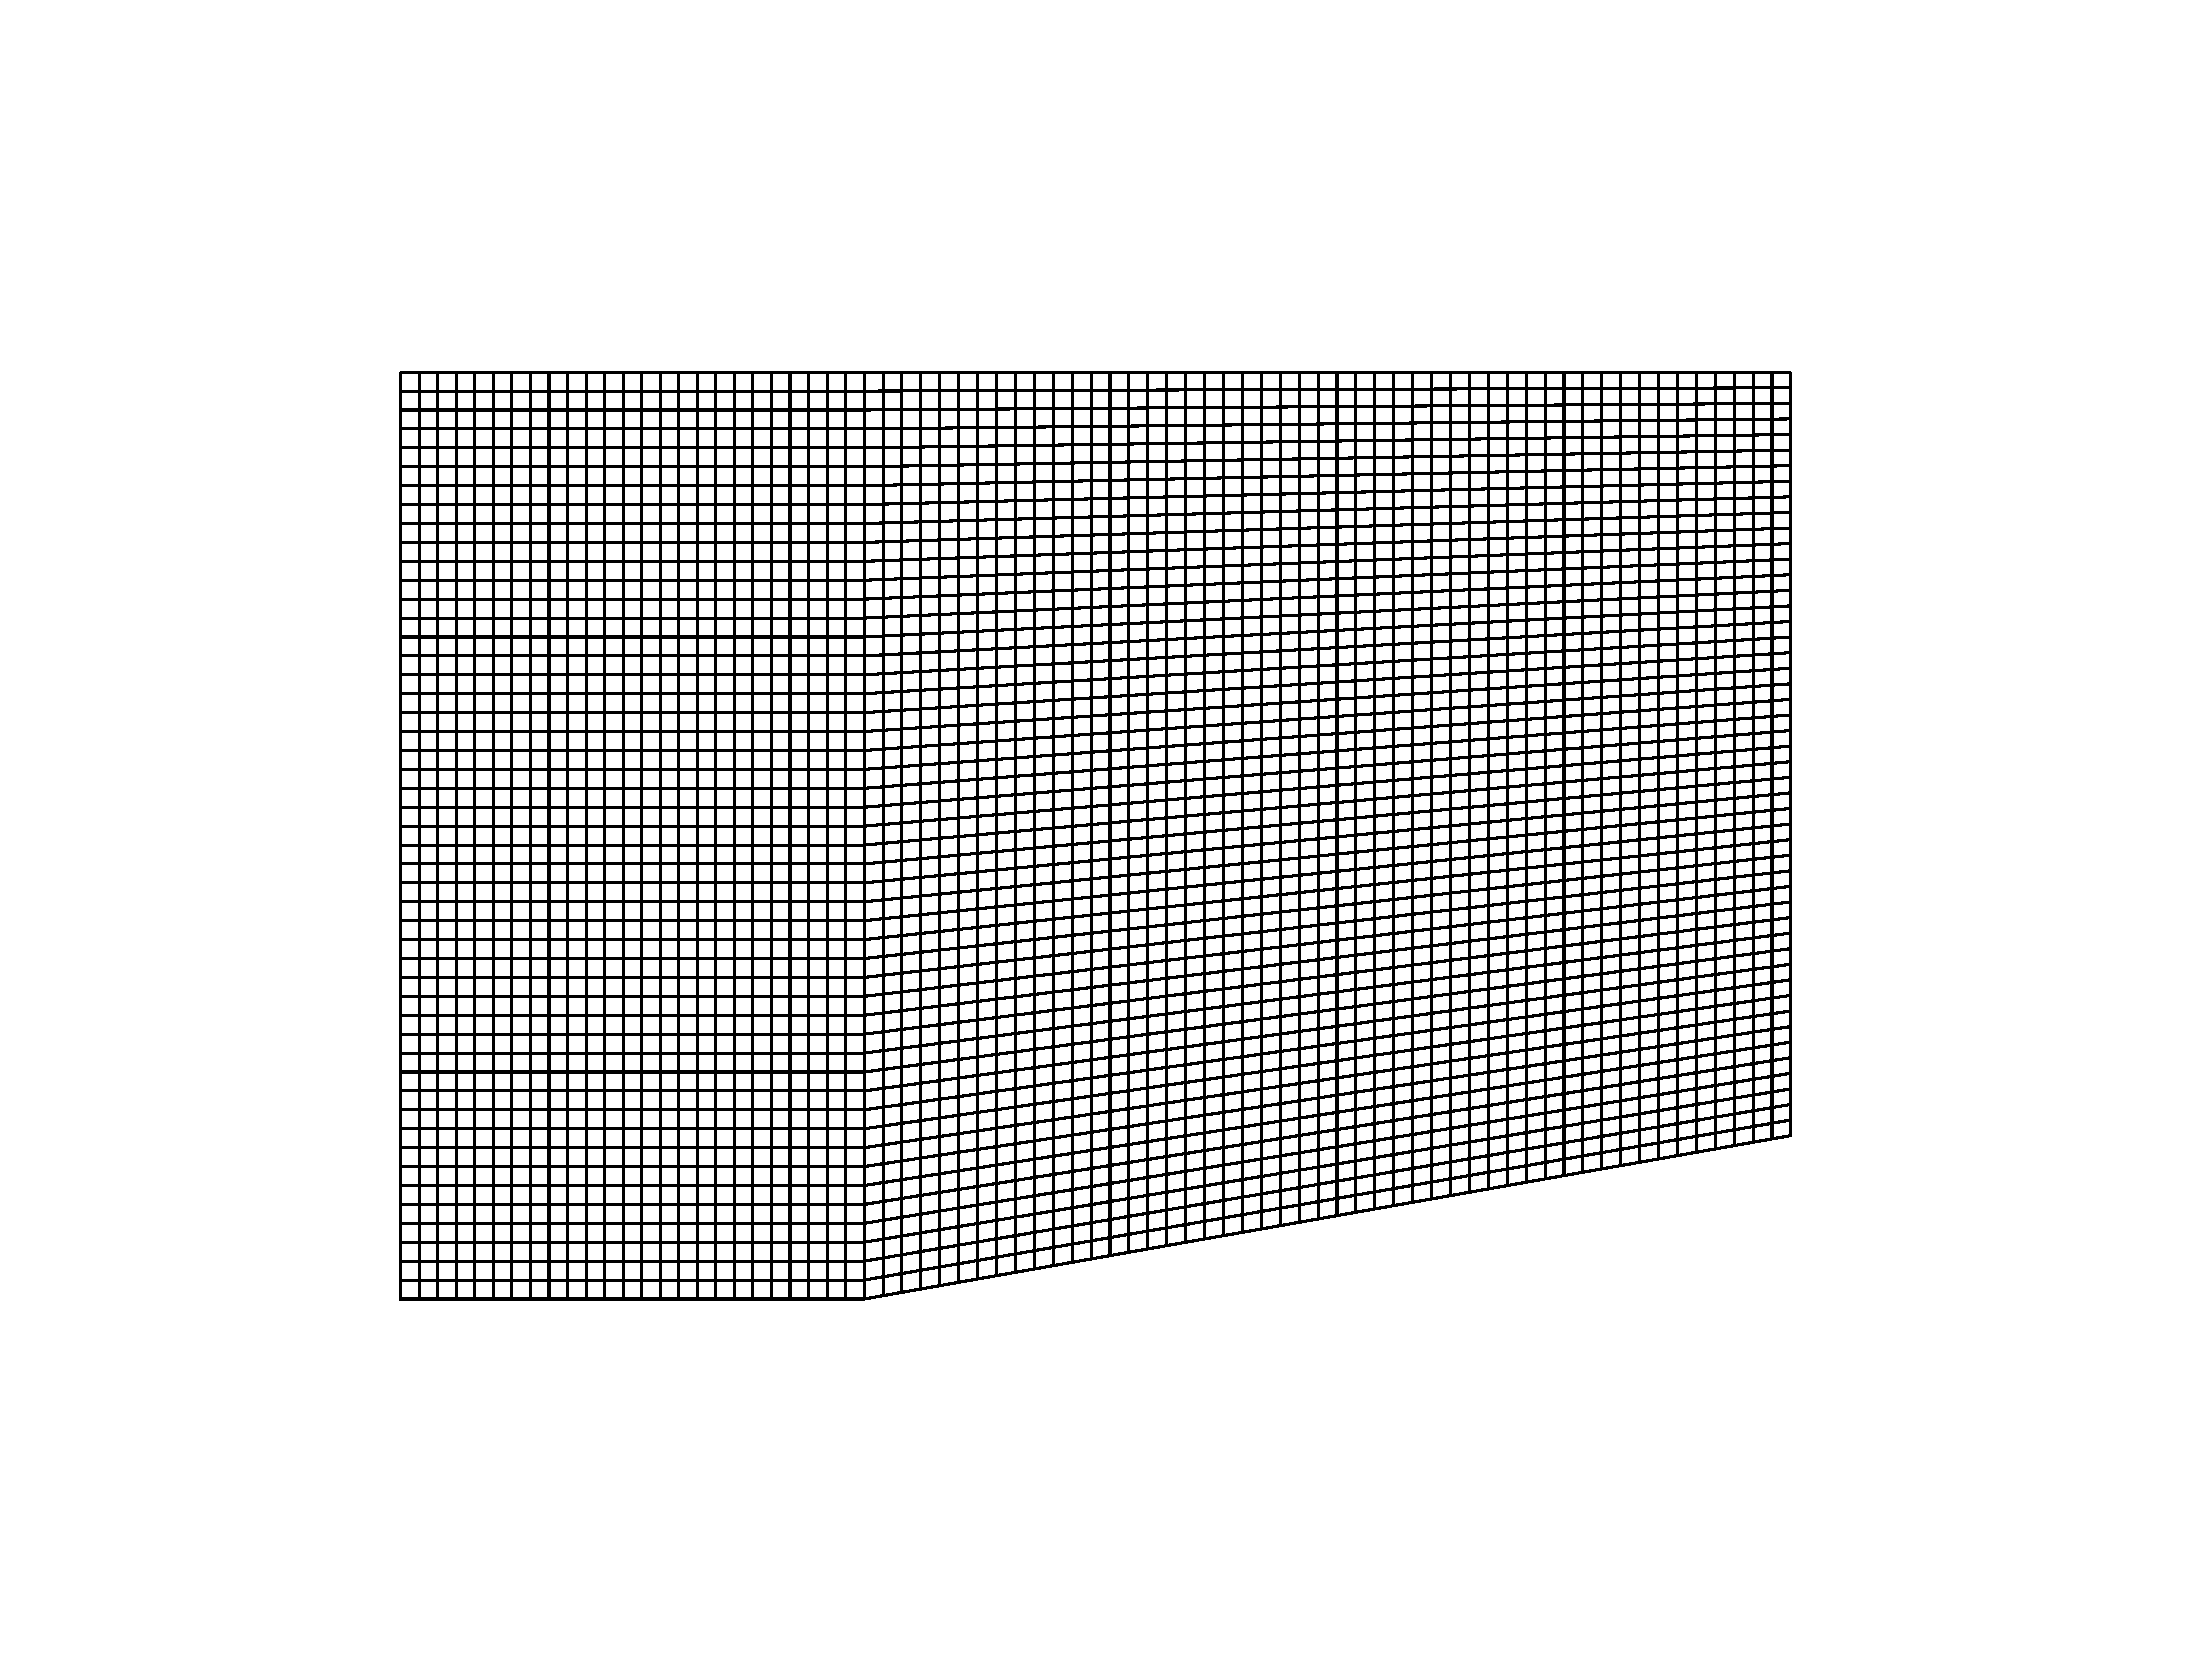
\includegraphics[width=.75\textwidth]{tut02/mesh.pdf}
    \caption{The structured mesh for the supersonic wedge.}
    \label{fig2:mesh}
\end{figure}
%--------------------------------------------------------------
\subsection{Visualize Pressure and Mach Contours}
To display pressure contours, you can take the following steps:
\begin{enumerate}[label=\arabic*)]
	\item Click on \texttt{flow.vtk} in the \textbf{Pipeline Browser}, and then click on the \textbf{Display} form in the \textbf{Properties} tab.
	\item Under the \textbf{Coloring} section select \textit{Pressure} from the drop-down menu (Figure \ref{fig2:pressure contours setting}).
\end{enumerate}
\begin{figure}[H]
	\centering
	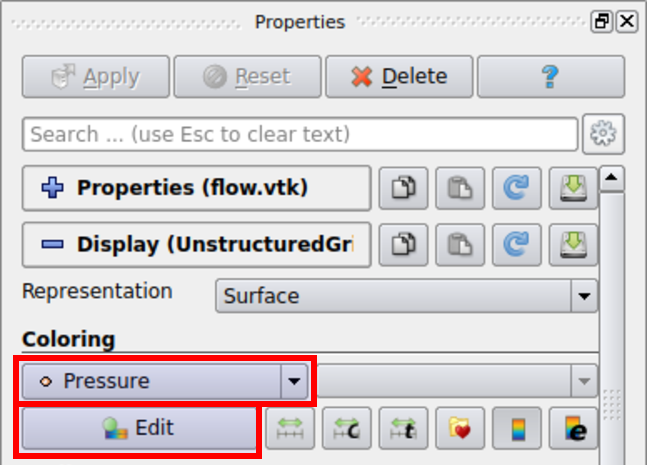
\includegraphics[width=0.4\textwidth]{tut02/pressurecont.pdf}
	\caption{Settings for displaying pressure contours.}
	\label{fig2:pressure contours setting}
\end{figure} 
\begin{enumerate}[label=\arabic*)]
	\setcounter{enumi}{2}
	\item Additionally, to change the color settings used for pressure you can click on the \textbf{Edit} option under the \textbf{Coloring} section. Another display window will appear on the right-hand side of the menu entitled \textbf{Mapping Data}, similar to Figure \ref{fig2:color_range}. Now you can change contour colors by choosing \textbf{Choose preset}.
\end{enumerate}  
\begin{figure}[ht]
    \centering
    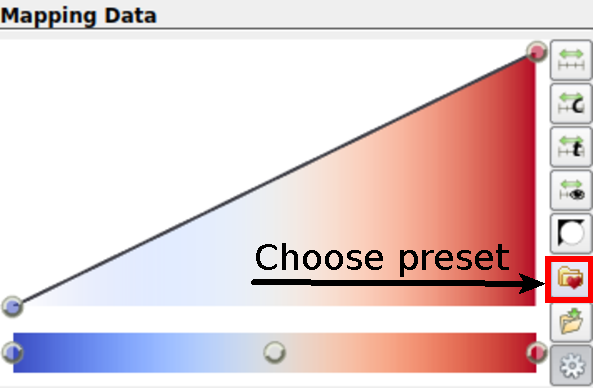
\includegraphics[width=0.4\textwidth]{tut02/colorrange.pdf}
    \caption{Changing the color range used for pressure contours.}
    \label{fig2:color_range}
\end{figure}
\begin{enumerate}[label=\arabic*)]
	\setcounter{enumi}{3}
	\item Choose a color scale for your contours. Here, we select the \textit{Cold and Hot} color scale, to be able to show clearly the sharp changes in pressure values around the shock (Figure \ref{fig2:color_range_item}). Then, click \textbf{Apply}.
\end{enumerate}  
\begin{figure}[ht]
    \centering
    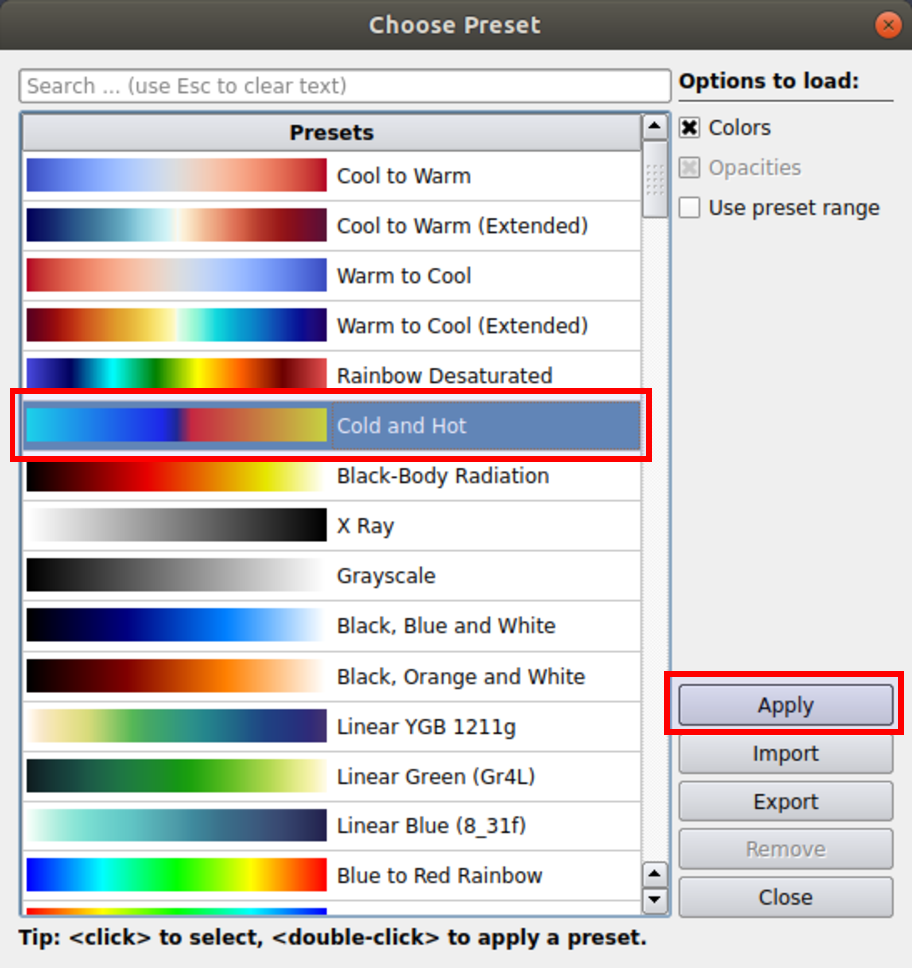
\includegraphics[width=0.45\textwidth]{tut02/changecontourcolors.pdf}
    \caption{Different color ranges used to display contours.}
    \label{fig2:color_range_item}
\end{figure}
\begin{enumerate}[label=\arabic*)]
	\setcounter{enumi}{4}
	\item To add axes to the plots look under the \textbf{Miscellaneous} form of the \textbf{Display} field (Figure \ref{fig2:add axis}) and select the check box beside \textbf{Data Axes Grid}. Then go to \textbf{Edit} and change these options based on your preferences (Figure \ref{fig2:axis setting}). Finally, the pressure contour you get should be similar to Figure \ref{fig2:plot pressure cont1}.
\end{enumerate}
\begin{figure}[H]
    \centering
    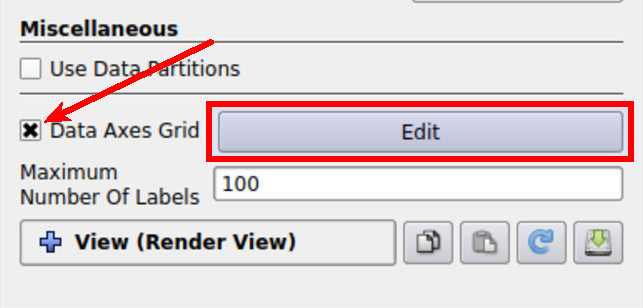
\includegraphics[width=0.4\textwidth]{tut02/addaxis.pdf}
    \caption{How to add axes to the plots.}
    \label{fig2:add axis}
\end{figure}
\begin{figure}[ht]
    \centering
    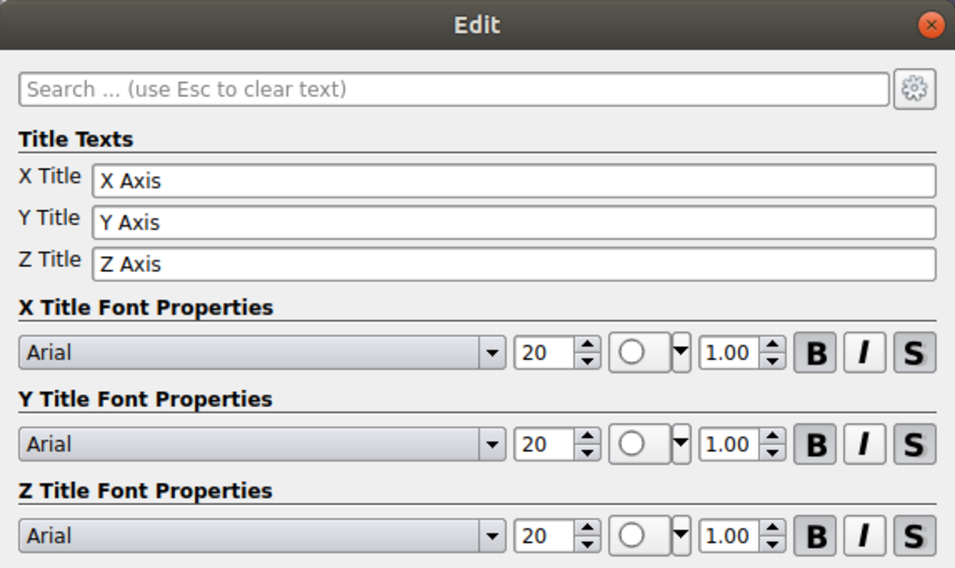
\includegraphics[width=0.6\textwidth]{tut02/axissettings.pdf}
    \caption{Settings for the axis style.}
    \label{fig2:axis setting}
\end{figure}
\begin{figure}[ht]
    \centering
    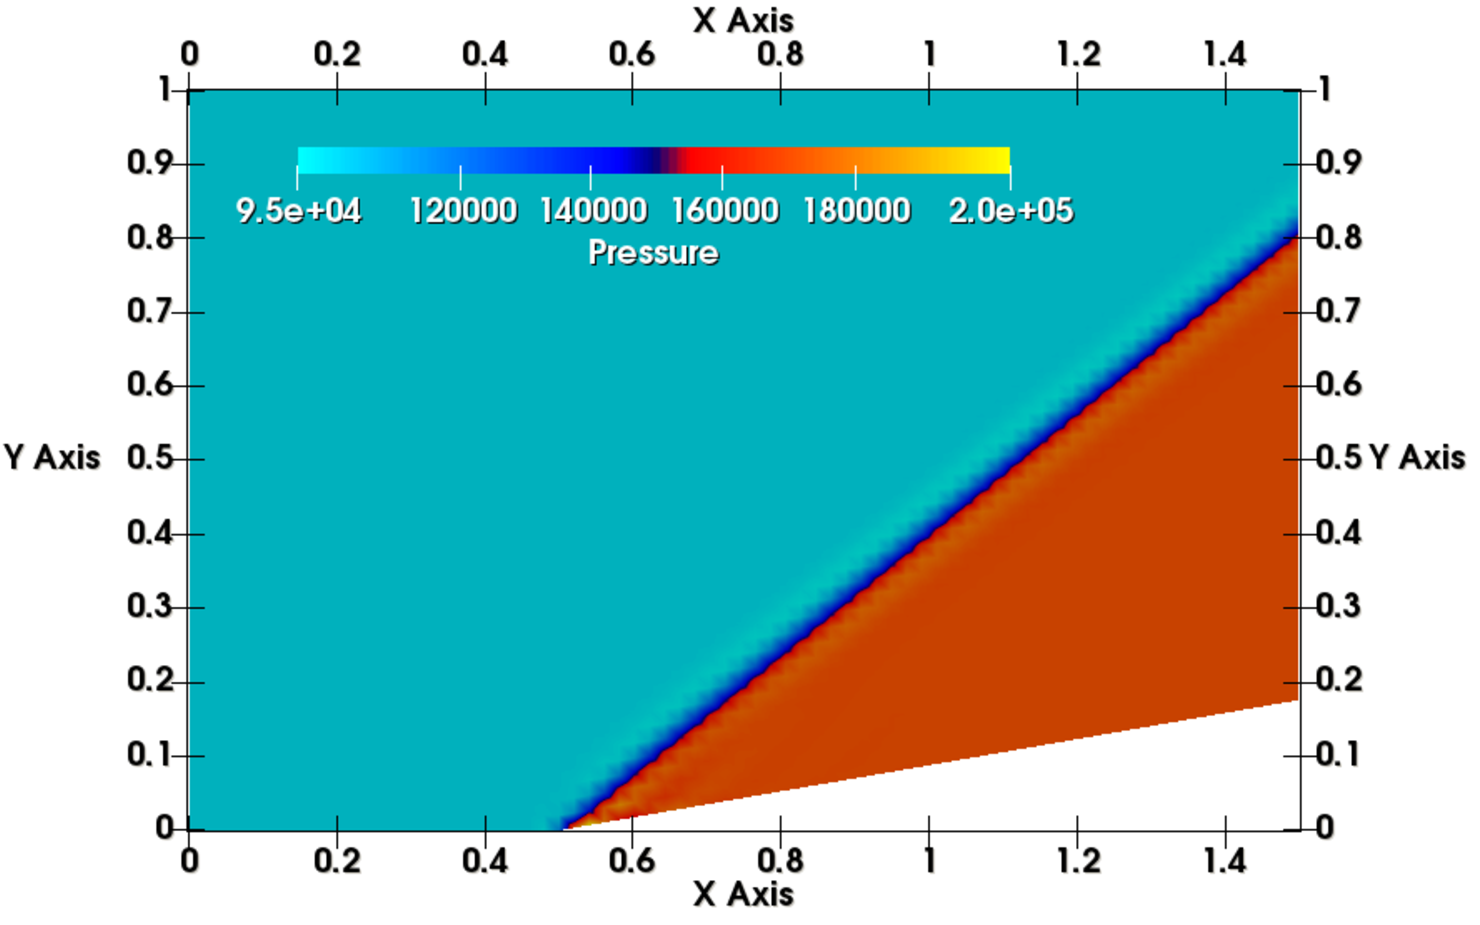
\includegraphics[width=0.85\textwidth]{tut02/plot1pressurecont.pdf}
    \caption{Pressure contours for the supersonic wedge case.}
    \label{fig2:plot pressure cont1}
\end{figure}
%----------------------------------------------------------

The pressure gradient along the shock wave is difficult to visualize directly from these contours. To help, we can add contour lines to clearly delineate the different regions. To add contour lines, you can take the following steps:
\begin{enumerate}[label=\arabic*)]
	\setcounter{enumi}{5}
	\item Click on the \texttt{flow.vtk} file in the \textbf{Pipeline Browser}, and then click on the \textbf{Contour} icon (Figure \ref{fig2:contour_icon}) in the toolbar. Now a new \textit{Contour1} item appears under the \texttt{flow.vtk} file in the \textbf{Pipeline Browser} (Figure \ref{fig2:contour1}). Click on \textbf{Apply} to proceed to the next step.
\end{enumerate}
\begin{figure}[H]
    \centering
    \includegraphics[width=0.5\textwidth]{tut02/contourlineicon.pdf}
    \caption{\textbf{Contour} icon in the toolbar.}
    \label{fig2:contour_icon}
\end{figure}
\begin{figure}[ht]
    \centering
    \includegraphics[width=0.4\textwidth]{tut02/contour1.pdf}
    \caption{Adding \textit{Contour1} to the \textbf{Pipeline Browser}.}
    \label{fig2:contour1}
\end{figure}
\begin{figure}[ht]
	\centering
	\begin{subfigure}[b]{.4\textwidth}
		\centering
		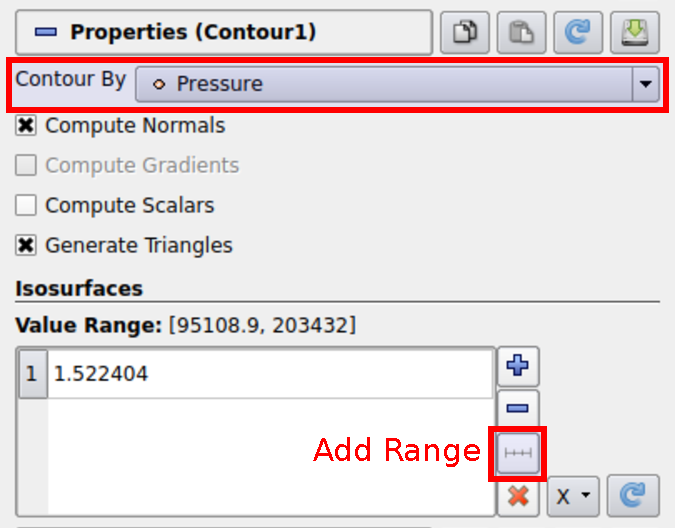
\includegraphics[width=1.0\textwidth]{tut02/contourby.pdf}
		\caption{Define a new range}
		\label{fig2:contourby a}
	\end{subfigure}
	\hfill
	\begin{subfigure}[b]{.4\textwidth}
		\centering
		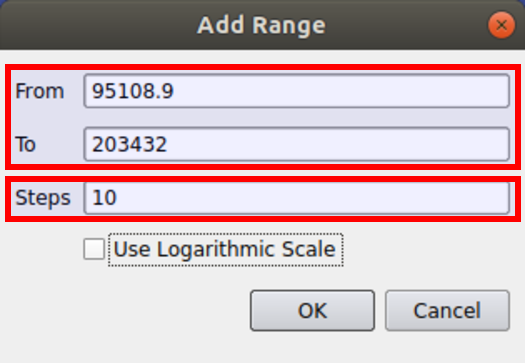
\includegraphics[width=1.0\textwidth]{tut02/addrange.pdf}
		\caption{Add range}
		\label{fig2:contourby b}
	\end{subfigure}     
	\caption{How to define a new range for the contour lines.}
	\label{fig2:contourby}
\end{figure}
\begin{enumerate}[label=\arabic*)]
	\setcounter{enumi}{6}
	\item With regard to Figure \ref{fig2:contourby a}, go to the \textbf{Properties} tab and select \textit{Pressure} from the \textbf{Contour By} drop-down menu.
	\item Click on the \textbf{Add Range} icon to customize the range to be used for the pressure contours. In Figure \ref{fig2:contourby b}, you will see the max/min range of contour lines (i.e. \textbf{From}/\textbf{To}), as well as number of lines you would like to have in your contour plot (i.e. \textbf{Steps}).
	\item Next, set \textbf{Steps} to 20, and click \textbf{OK}. By doing this the pressure contour range is equally divided into 20 lines. At the end, click on \textbf{Apply} to see contour lines in the display window.
	\item As shown in Figure \ref{fig2:colorby2}, click on \textbf{Display} under the \textbf{Properties} tab. In the \textbf{Coloring} section select \textbf{Solid Color} from the drop-down menu and choose white from \textbf{Edit}. The pressure contour lines should now be similar to those in Figure \ref{fig2:pressure_contour_lines}. You can zoom-in to the region at the bottom of the wedge to see the pressure gradient along the oblique
	shock, as shown in Figure \ref{fig2:pressure_contour_lines_zoom}.
\end{enumerate}





\begin{figure}[ht]
    \centering
    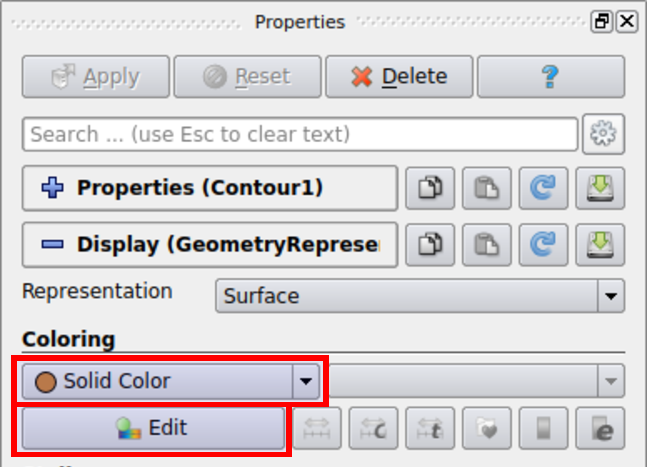
\includegraphics[width=0.4\textwidth]{tut02/contourline.pdf}
    \caption{Changing contour line colors in the \textbf{Coloring} section.}
    \label{fig2:colorby2}
\end{figure}

\begin{figure}[ht]
    \centering
    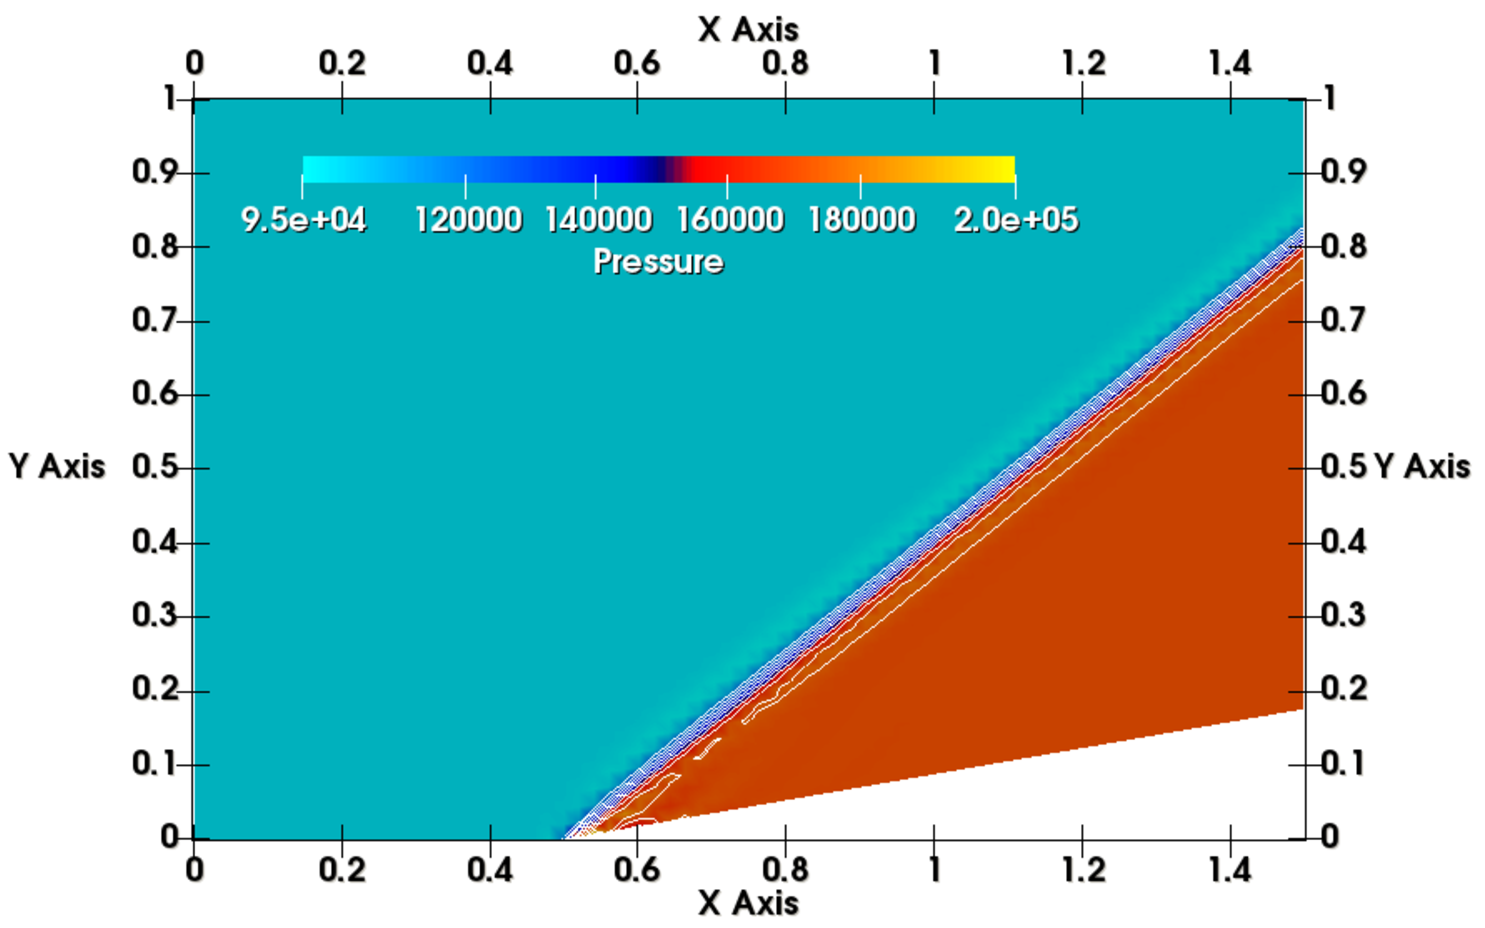
\includegraphics[width=.85\textwidth]{tut02/plot2pressurecont.pdf}
    \caption{Pressure contours superimposed by contour lines for the supersonic wedge case.}
    \label{fig2:pressure_contour_lines}
\end{figure}
\begin{figure}[H]
    \centering
    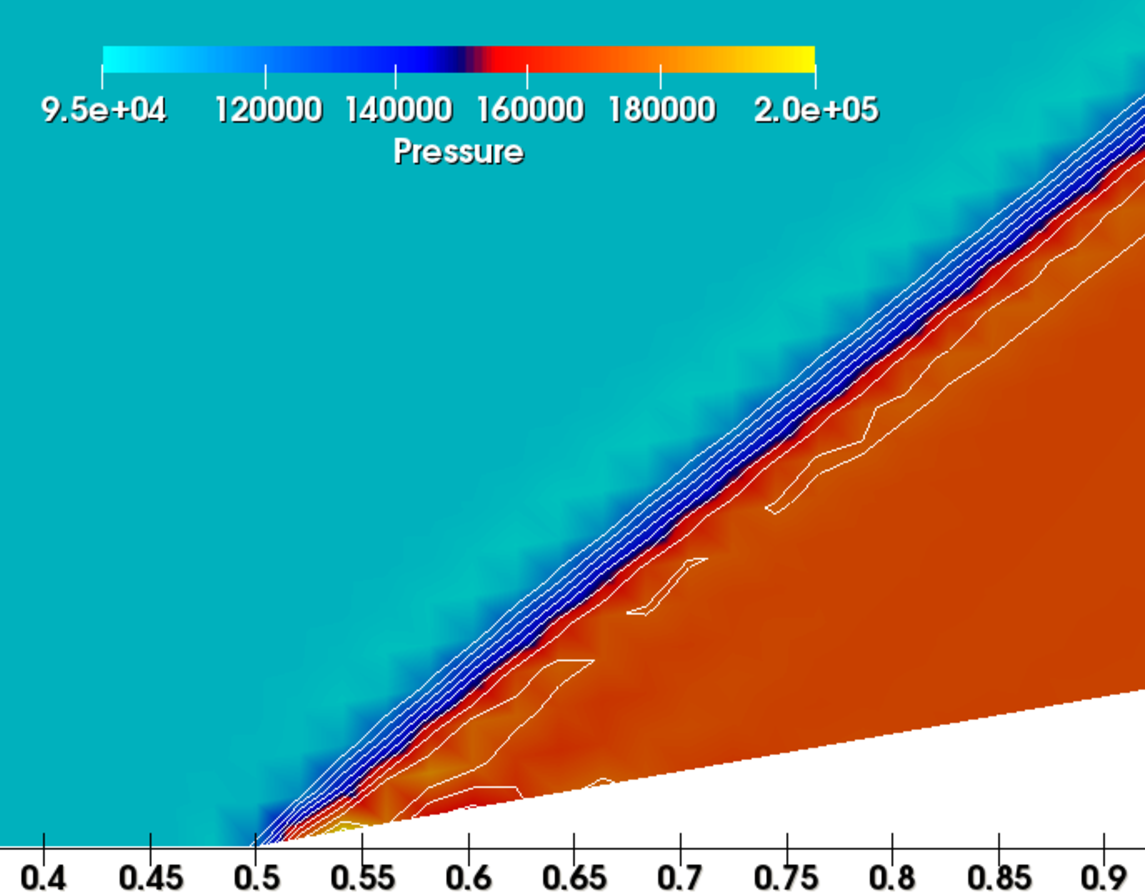
\includegraphics[width=.65\textwidth]{tut02/plot3pressurecont.pdf}
    \caption{Magnified pressure contour superimposed with contour lines for the supersonic wedge case.}
    \label{fig2:pressure_contour_lines_zoom}
\end{figure}
\begin{enumerate}[label=\arabic*)]
	\setcounter{enumi}{9}
	\item Now to display the Mach number contours click on \texttt{flow.vtk} in the \textbf{Pipeline Browser}.
	\item Similar to Figure \ref{fig2:pressure contours setting}, under the \textbf{Coloring} section select \textit{Mach} from the drop-down menu.
	\item Click on \textit{Contour1} in the \textbf{Pipeline Browser}. Now, under \textbf{Properties} select \textit{Mach} from the \textbf{Contour By} drop-down menu.
	\item Since all these settings are related to the previous pressure values we need to revise some options to display contours of \textit{Mach} number appropriately. To do this we need to delete the data range that was used for pressure, and replace it with the data range of the Mach number. Under \textbf{Isosurfaces} from \textbf{Properties}, click on the \textbf{Remove All} icon, and then click on the \textbf{Add Range} icon, as shown in Figure \ref{fig2:contourby2 a}. As you can see from Figure \ref{fig2:contourby2 b}, the max/min values for mach number has changed.
	\item Set the \textbf{Steps} to 20 and click on \textbf{OK} to proceed to the next step. Now the Mach number contours should look similar to Figure \ref{fig2:mach_contour}. Additionally, if you zoom-in the plot you will see more contour details near the wedge, similar to Figure \ref{fig2:mach_contour_zoom}.
\end{enumerate}
\begin{figure}[ht]
    \centering
     \begin{subfigure}[b]{.4\textwidth}
         \centering
         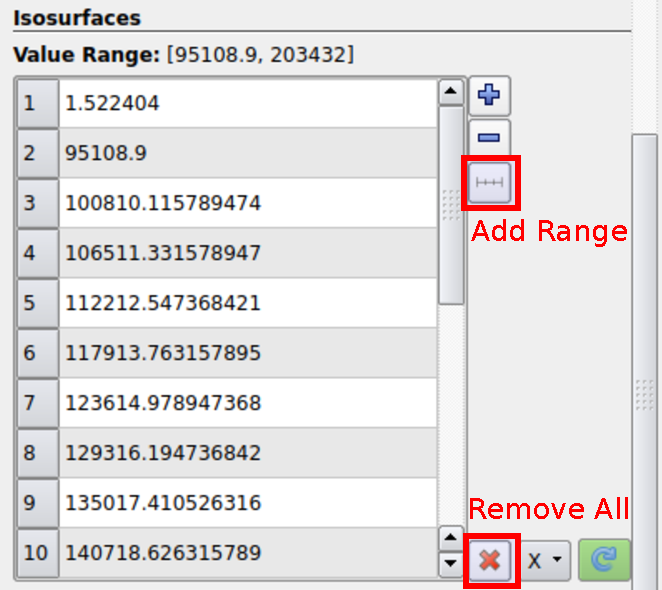
\includegraphics[width=1.0\textwidth]{tut02/deladdrange.pdf}
         \caption{Define a new contour range}
         \label{fig2:contourby2 a}
     \end{subfigure}
     \hfill
     \begin{subfigure}[b]{.4\textwidth}
         \centering
         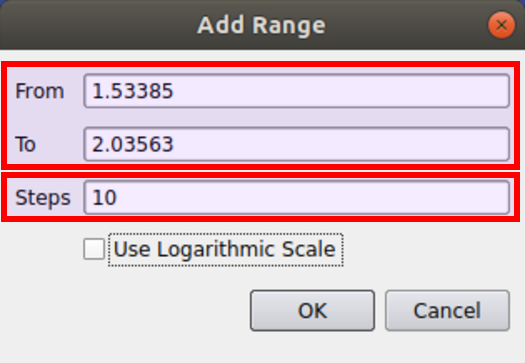
\includegraphics[width=1.0\textwidth]{tut02/addrange2.pdf}
         \caption{Add range}
         \label{fig2:contourby2 b}
     \end{subfigure}     
    \caption{Define a new range for the contour lines.}
    \label{fig2:contourby2}
\end{figure}
\begin{figure}[ht]
    \centering
    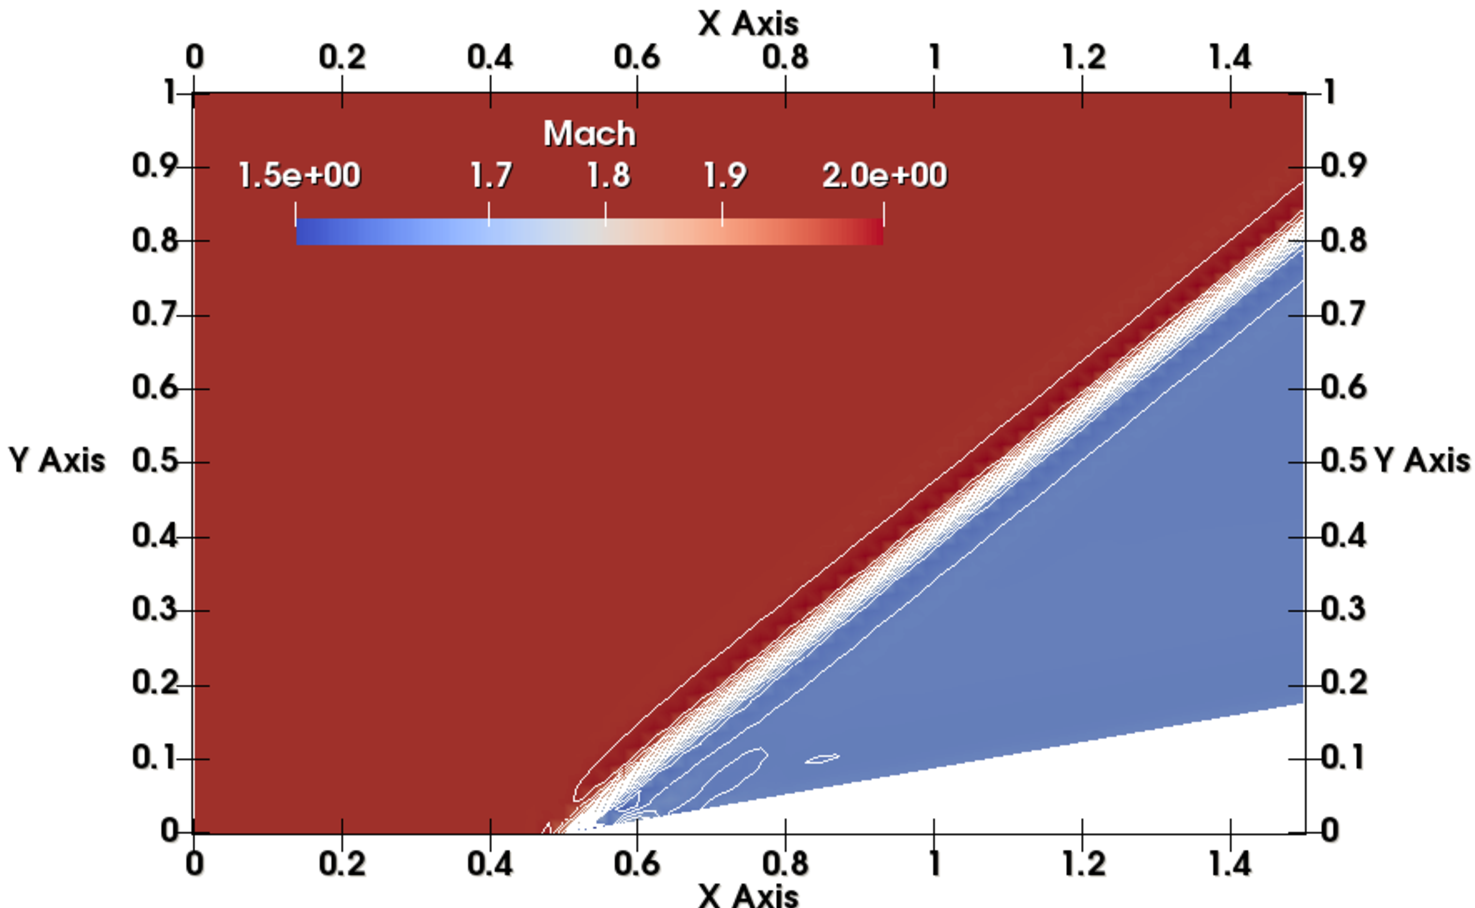
\includegraphics[width=.75\textwidth]{tut02/plot1machcont.pdf}
    \caption{Mach number contours superimposed with contour lines for the supersonic wedge case.}
    \label{fig2:mach_contour}
\end{figure}
\begin{figure}[ht]
    \centering
    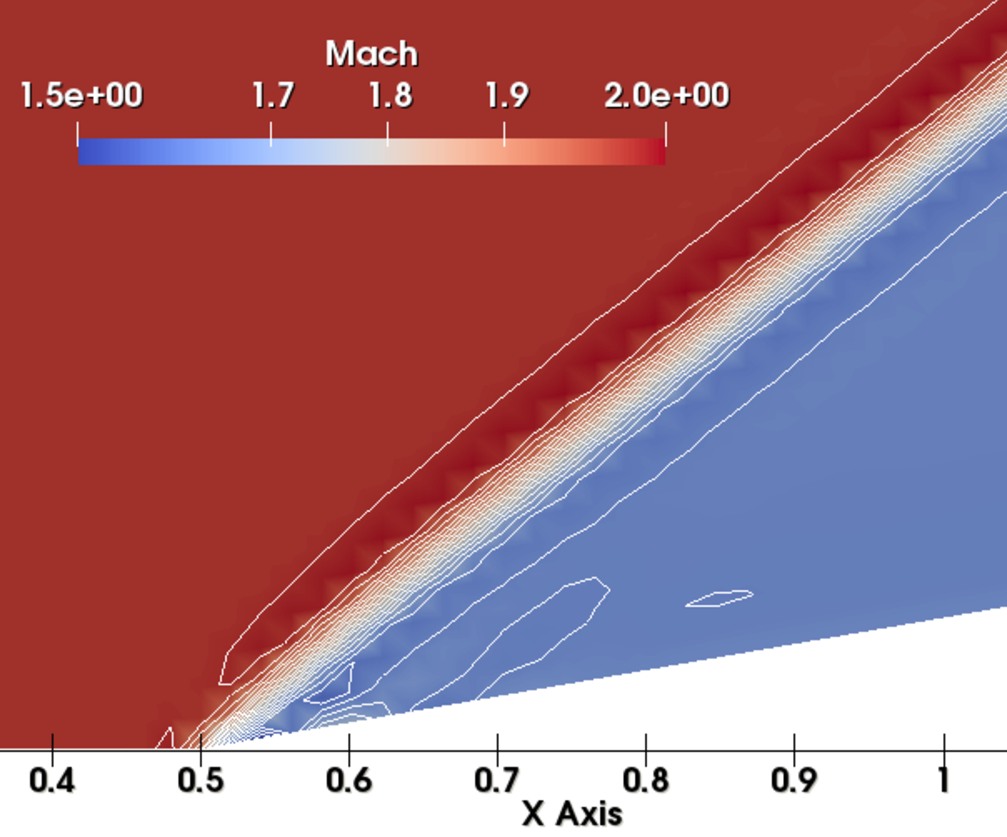
\includegraphics[width=.55\textwidth]{tut02/plot1machcont2.pdf}
    \caption{Magnified Mach number contours superimposed with contour lines for the supersonic wedge case.}
    \label{fig2:mach_contour_zoom}
\end{figure}
%--------------------------------------------------------------
\subsection{Plotting a variable over an arbitrary line}
To plot a variable over an arbitrary line in space you can take the following steps:
\begin{enumerate}[label=\arabic*)]
	\setcounter{enumi}{0}
	\item Select \texttt{flow.vtk} by clicking on it in the \textbf{Pipeline Browser}.
	\item Go to \textbf{Filters} $\rightarrow$  \textbf{Data Analysis} $\rightarrow$  \textbf{Plot Over Line} (as shown in Figure \ref{fig2:plot_over_line}).
	\item Under \textbf{Line Parameters} in \textbf{Properties} (as shown in Figure \ref{fig2:line_coordinate}), select the coordinates for two arbitrary points you want (i.e. \textbf{Point1} and \textbf{Point2}). In this case, plot the line from \textbf{Point1} to \textbf{Point2} with (0,0.5,0) and (1.5,0.5,0), respectively, and then click \textbf{Apply}. A new line plot item will be generated.
\end{enumerate}
\begin{figure}[H]
	\centering
	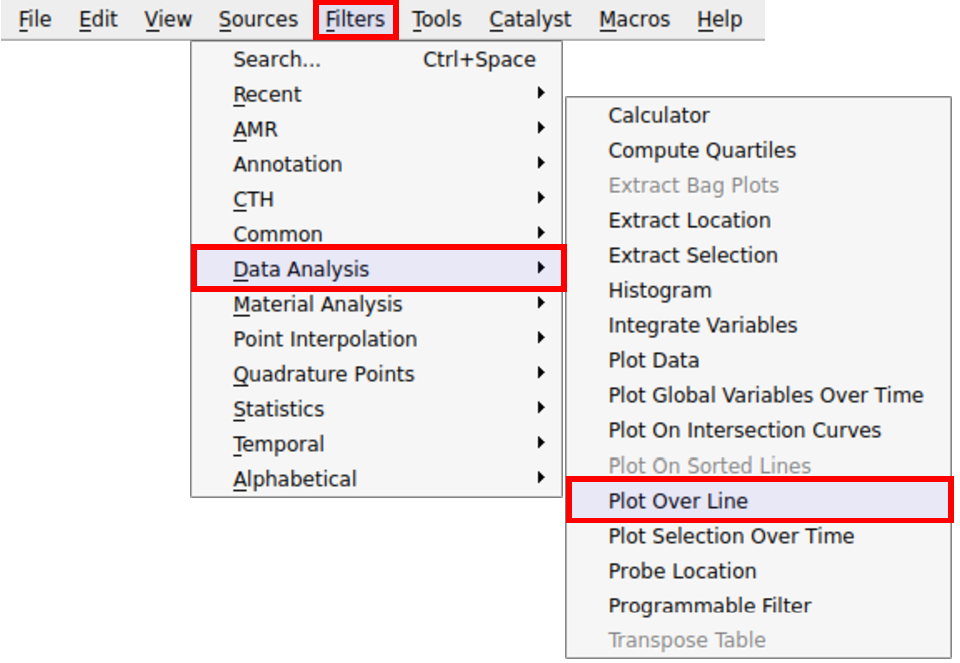
\includegraphics[width=.6\textwidth]{tut02/plotoverline.pdf}
	\caption{How to plot data over an arbitrary line in space.}
	\label{fig2:plot_over_line}
\end{figure}
\begin{figure}[ht]
	\centering
	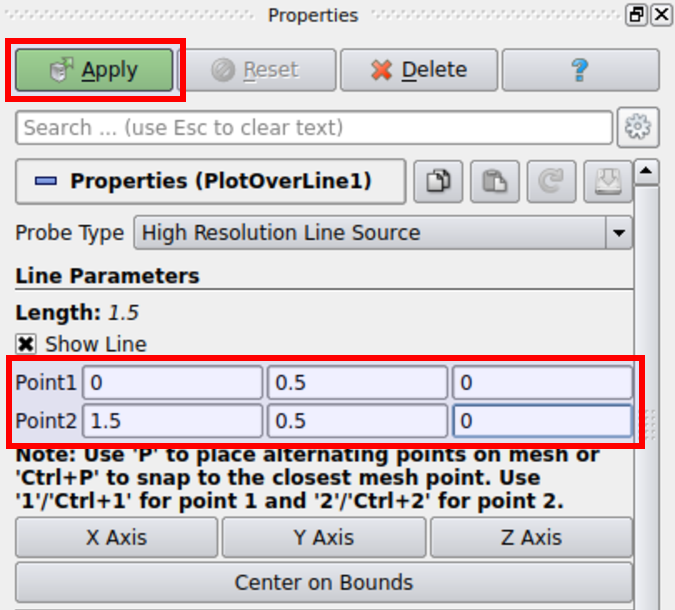
\includegraphics[width=.4\textwidth]{tut02/linecoord.pdf}
	\caption{Define the coordinates for a line plot in space.}
	\label{fig2:line_coordinate}
\end{figure}
\begin{enumerate}[label=\arabic*)]
	\setcounter{enumi}{3}
	\item  According to Figure \ref{fig2:plot_line_setting}, under the \textbf{X Axis Parameters} from \textbf{Display}, select \textit{Point\_X} from the \textbf{X Array Name} drop-down menu. Now, under the \textbf{Series Parameters} options toggle the box beside \textbf{Variable} to uncheck everything, then select only the \textit{Mach} item. The plot of Mach number vs the \textit{x-coordinate} will be displayed in the main window as shown in Figure \ref{fig2:plot_line}.
\end{enumerate}
\begin{figure}[H]
	\centering
	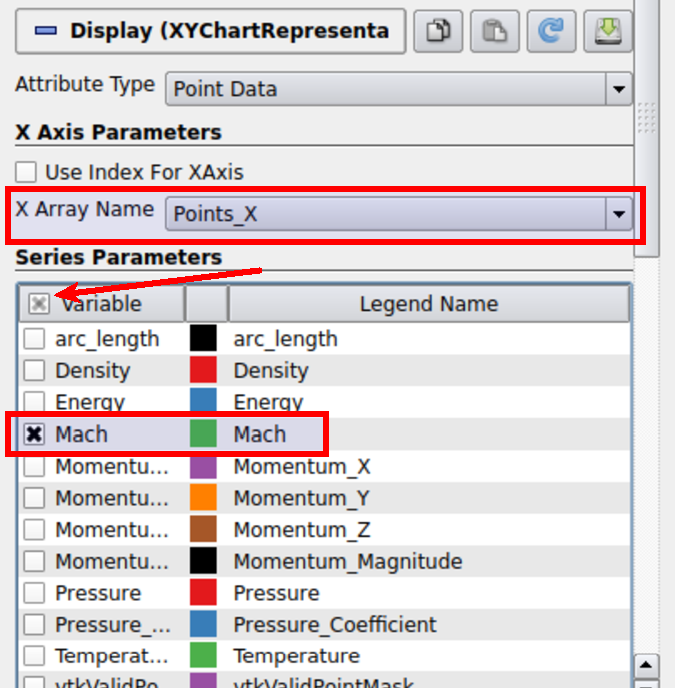
\includegraphics[width=.45\textwidth]{tut02/plotmachline.pdf}
	\caption{How to plot Mach number over a line.}
	\label{fig2:plot_line_setting}
\end{figure}
\begin{figure}[ht]
	\centering
	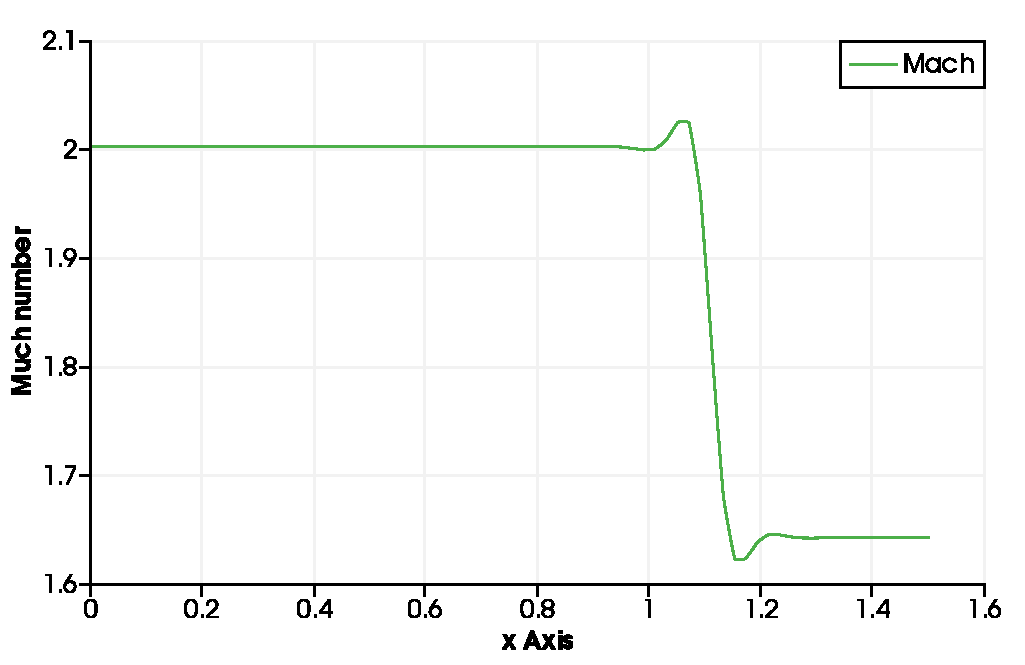
\includegraphics[width=.85\textwidth]{tut02/plot2contourline.pdf}
	\caption{Mach number plotted over the specified line.}
	\label{fig2:plot_line}
\end{figure}
\begin{enumerate}[label=\arabic*)]
	\setcounter{enumi}{5}
	\item In order to see a spreadsheet view of the datapoints you can click the upper right icon as shown in Figure \ref{fig2:open_spreadsheet}, then click on the \textit{Spreadsheet View} similar to Figure \ref{fig2:spreadsheet}.
	\item Additionally, you can export a .csv file and plot it with any other plotting software. To export the spreadsheet as a .csv file, go to \textbf{File} $\rightarrow$ \textbf{Export}, and then \textbf{Save as} .csv.
\end{enumerate}
\begin{figure}[ht]
    \centering
    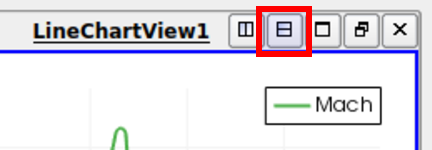
\includegraphics[width=.4\textwidth]{tut02/openspreadsheet.pdf}
    \caption{How to make spreadsheet view in a new window.}
    \label{fig2:open_spreadsheet}
\end{figure}
\begin{figure}[ht]
    \centering
    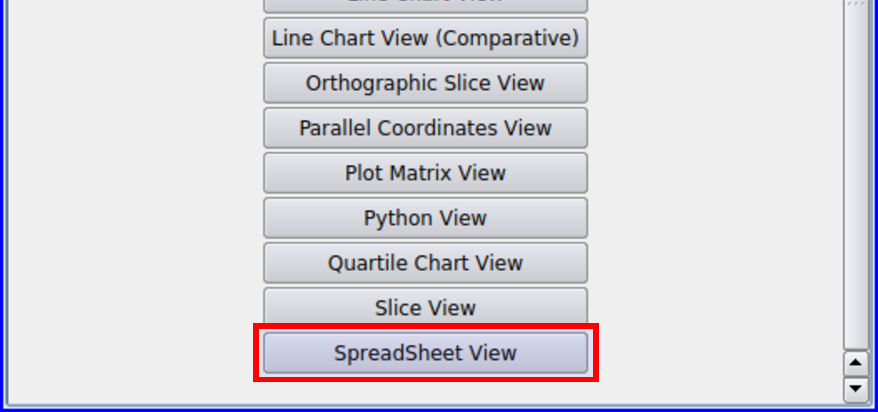
\includegraphics[width=.65\textwidth]{tut02/spreadsheet.pdf}
    \caption{Selecting the \textit{Spreadsheet View} among the different available views.}
    \label{fig2:spreadsheet}
\end{figure}

%++++++++++++++++++++++++++++++++++++++++++++++++++++++++++++++
\section{Questions}
1. Run the default case as provided which uses 2ND\_ORDER and the HLLC Riemann solver.
\begin{enumerate}[label=(\alph*)]
    \item Create coloured contours of Pressure and Mach number in the entire domain.
    \item Plot Pressure from (0,0.5,0) to (1.5,0.5,0) using \textbf{Plot Over Line}.
\end{enumerate}
2. Repeat Q.1 but switch the SPATIAL\_ORDER\_FLOW to 1ST\_ORDER. \\
3. Repeat 1 using SPATIAL\_ORDER\_FLOW as 2ND\_ORDER but using the JST flux. \\
4. Repeat Q.1 using SPATIAL\_ORDER\_FLOW as 2ND\_ORDER but using the LAX-FRIEDRICH flux. \\
5. Repeat Q.1 using SPATIAL\_ORDER\_FLOW as 2ND\_ORDER but using the CUSP flux. \\
6. Repeat Q.1 using SPATIAL\_ORDER\_FLOW as 2ND\_ORDER but using the ROE flux. \\
7. Comment on how the spatial order of accuracy and choice of Riemann solver affect the resolution of the shock and any dissipation or dispersion errors you can observe. Based on your results, recommend a combination of spatial order and Riemann solver that performs particularly well.
%++++++++++++++++++++++++++++++++++++++++++++++++++++++++++++++
%++++++++++++++++++++++++++++++++++++++++++++++++++++++++++++++
%++++++++++++++++++++++++++++++++++++++++++++++++++++++++++++++
\chapter{Inviscid ONERA M6}
\label{ch:Inviscid ONERA M6}
%++++++++++++++++++++++++++++++++++++++++++++++++++++++++++++++
\section{Required Files}
\begin{su2note}
	Use the following links to download the same version of SU2 for Windows (\href{https://users.encs.concordia.ca/~bvermeir/book/executables/windows/SU2_Windows.zip}{\underline{click here}}) or Mac (\href{https://users.encs.concordia.ca/~bvermeir/book/executables/osx/SU2_Mac.zip}{\underline{click here}}), and the required configuration and mesh files (\href{https://gitlab.com/bvermeir/book-cfd/blob/master/tutorial/tut3_invisicd_oneram6/oneram6_inviscid.zip}{\underline{click here}}).
\end{su2note}
\begin{paraviewnote}
	Use the following links to download the same version of Paraview for Windows (\href{https://users.encs.concordia.ca/~bvermeir/book/executables/windows/ParaView-5.4.0-Qt5-OpenGL2-Windows-64bit.exe}{\underline{click here}}) or Mac (\href{https://users.encs.concordia.ca/~bvermeir/book/executables/osx/ParaView-5.4.0-Qt5-OpenGL2-MPI-OSX10.8-64bit.dmg}{\underline{click here}}).
\end{paraviewnote}

\section{Problem Description}
In this tutorial, we are going to explain how to simulate transonic inviscid flow around the three-dimensional ONERA M6 wing. This is a commonly used benchmark problem for computational aerodynamics, due to the availability of experimental data and its relatively simple geometry. In this tutorial the computational domain is discretized using an unstructured mesh with of 582,752 tetrahedral elements. The flow specification is as follows:
\begin{itemize}
    \item Pressure = 101,325 Pa
    \item Temperature = 273.15 K
    \item Mach number = 0.8395
    \item angle of attack = 3.06 degrees
\end{itemize}

This tutorial has two parts: Flow Solution and Post-processing. In the first part, we will explain how to manage the prerequisite files and settings, and how to run the CFD simulation using SU2. In the second part we explain how to use Paraview to visualize the data obtained from SU2.
%++++++++++++++++++++++++++++++++++++++++++++++++++++++++++++++
\section{Flow solution}
In the configuration file you can manually adjust the multi-grid control parameters. For the tutorial case you will see that the number of multigrid levels is set to 0, \texttt{MGLEVEL=0}. In the assigned questions the number of multigrid levels will be changed by adjusting this \texttt{MGLEVEL} parameter. You can also select the multi-grid cycle type by choosing one of either \texttt{MGCYCLE (V Cycle, W Cycle or Full MG Cycle)}. Another parameter that can be controlled is the total number of iterations. This can be modified by changing the value of \texttt{EXT\_ITER}. For this example it will be kept at 200 for demonstration purposes, but depending on the method used more iterations may be required to reach convergence. We will post-process the results by obtaining pressure coefficient and Mach number contours, the lift coefficient ($C_L$), and drag coefficient ($C_D$) of the ONERA M6 wing. We will also explore the rate of convergence as a function of the number of multigrid levels used.

To run the simulation SU2 needs two files: the configuration file (\texttt{.cfg}) and the mesh file (\texttt{.su2}). Links to the required files and executables are provided at the start of this tutorial. The files include:
\begin{enumerate}
\item \texttt{inv\_ONERAM6\_JST.cfg} as a configuration file.
\item \texttt{mesh\_ONERAM6\_inv.su2} as a mesh file.
\end{enumerate}
The next step is to copy these two files into the same directory as your SU2 executable. Then open a terminal window and execute the following commands to run the simulation:
\begin{table}[ht]
    \centering
    \begin{tabular}{|l|l|}
    \hline
    Windows     & \begin{tabular}{c} \$ cd "where you saved the package" \\ \$ SU2\_CFD.exe inv\_ONERAM6\_JST.cfg \end{tabular}
    \\
    \hline
    Mac     & \begin{tabular}{c} \$ cd "where you saved the package" \\ \$ ./SU2\_CFD inv\_ONERAM6\_JST.cfg \end{tabular}
    \\
    \hline
    \end{tabular}
\end{table}

The solver will begin solving the problem and will print out the residuals at every iteration, until the specified convergence criteria is achieved. The computational time for this case is highly dependant on the computer's performance. However, the run time is supposed to be about 5 hours on average. After the calculations are complete the following output files will be generated within in the SU2 folder:
\begin{itemize}
    \item \texttt{flow.vtk}: The flow solution on the entire domain.
    \item \texttt{force\_breakdown.dat}: Forces and moment on the airfoil.
    \item \texttt{history.vtk}: Convergence history.
    \item \texttt{restart\_flow.dat}: Restart file.
    \item \texttt{surface\_flow.vtk}: The flow solution on the airfoil surface.
    \item \texttt{surface\_flow.csv}: A comma separated value file of the flow solution on the airfoil.
\end{itemize}
Please keep in mind that every time you run SU2, the output data will be overwritten. Hence, before launching a new simulation you should backup your files in another directory.
%++++++++++++++++++++++++++++++++++++++++++++++++++++++++++++++
\section{Post-processing}
In this section, we will explain how to use Paraview to visualize the results produced by SU2.
%--------------------------------------------------------------
\subsection{Load the Solution File:}
In order to import the data to Paraview, you can take the following steps:
\begin{enumerate}[label=\arabic*)]
	\item Launch Paraview.
	\item Go to \textbf{File} $\rightarrow$ \textbf{Open}, and select the \texttt{surface\_flow.vtk} file.
	\item On the left-hand side of the Paraview window you will see the file is loaded under \textbf{builtin} in \textbf{Pipeline Browser}. Press the \textbf{Apply} button in the \textbf{Properties} tab, right under the \textbf{Pipeline Browser} heading. Paraview will now load the data associated with your file, and it will be ready for visualization (Figure \ref{fig3:load}).
\end{enumerate}
 
\begin{figure}[ht]
    \centering
    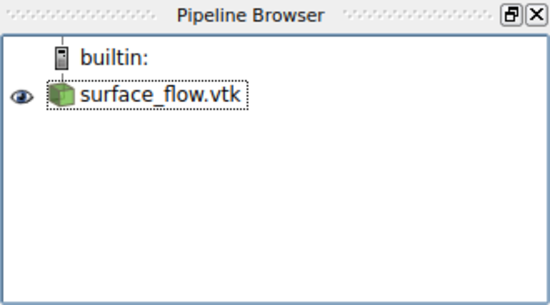
\includegraphics[width=0.4\textwidth]{tut03/surface_flow.pdf}
    \caption{Loading \texttt{surface\_flow.vtk} file into the \textbf{Pipeline Browser}.}
    \label{fig3:load}
\end{figure}
%--------------------------------------------------------------
\subsection{Visualize the Mesh}
In order to view the mesh, as shown in Figure \ref{fig3:wireframe}, select \textit{Solid Color} with \textit{Wireframe} in the toolbar. As you can see in Figure \ref{fig3:mesh}, the mesh around the ONERA M6 wing is unstructured and the elements are clustered around the wingtip, leading edge, and trailing edge of the wing. This is to accommodate large changes in the flow solution in the vicinity of the features.
\begin{figure}[ht]
    \centering
    \includegraphics[width=0.6\textwidth]{tut03/wireframe.pdf}
    \caption{How to display the ONERA M6 mesh.}
    \label{fig3:wireframe}
\end{figure}
\begin{figure}[ht]
    \centering
    \includegraphics[width=.75\textwidth]{tut03/mesh2.pdf}
    \caption{The unstructured mesh around the ONERA M6 wing.}
    \label{fig3:mesh}
\end{figure}
%--------------------------------------------------------------
\subsection{Pressure Coefficient and Mach Number Contours}
To display pressure coefficient contours on the surface of the wing, you can take the following steps:
\begin{enumerate}[label=\arabic*)]
	\item Click on \texttt{surface\_flow.vtk} in the \textbf{Pipeline Browser}.
	\item Click on \textbf{Display} in \textbf{Properties} tab
	\item Under \textbf{Coloring}, select \textit{Pressure\_Coefficient} from the drop-down menu (Figure \ref{fig3:pressure_coeff_1})
	\item Pressure coefficient contours should now be displayed, similar to Figure \ref{fig3:plot_pressure_coeff}.
\end{enumerate}
\begin{figure}[ht]
    \centering
    \includegraphics[width=0.4\textwidth]{tut03/coloring.pdf}
    \caption{Display contours by selecting the appropriate variable.}
    \label{fig3:pressure_coeff_1}
\end{figure}
\begin{figure}[ht]
    \centering
    \includegraphics[width=0.65\textwidth]{tut03/cont1_pressure_coefficient.pdf}
    \caption{Pressure coefficient contour for ONERA M6 wing.}
    \label{fig3:plot_pressure_coeff}
\end{figure}
\begin{enumerate}[label=\arabic*)]
	\setcounter{enumi}{4}
	\item To add contour lines to the plot click on \texttt{surface\_flow.vtk} in the \textbf{Pipeline Browser}, and then click on the \textbf{Contour} icon (Figure \ref{fig3:contour_icon}) in the toolbar.
	\item The \textit{Contour1} item now appears under \texttt{flow.vtk} file in the \textbf{Pipeline Browser} (Figure \ref{fig3:contour1}). Click on \textbf{Apply} to proceed to the next step.
\end{enumerate}
\begin{figure}[ht]
    \centering
    \includegraphics[width=0.5\textwidth]{tut03/contourlineicon.pdf}
    \caption{\textbf{Contour} icon in toolbar.}
    \label{fig3:contour_icon}
\end{figure}
\begin{figure}[H]
    \centering
    \includegraphics[width=0.4\textwidth]{tut03/contour1.pdf}
    \caption{Adding \textit{Contour1} in the \textbf{Pipeline Browser}.}
    \label{fig3:contour1}
\end{figure}
\begin{enumerate}[label=\arabic*)]
	\setcounter{enumi}{6}
	\item As shown in Figure \ref{fig3:contourby a}, go to \textbf{Properties} and choose \textit{Pressure\_Coefficient} from \textbf{Contour By} drop-down menu
	\item Click on the \textbf{Add Range} icon to customize the range used for the pressure contours.
	\item As shown in Figure \ref{fig3:contourby b}, set the max/min (i.e. \textbf{From}/\textbf{To}) range of contour lines, as well as the number of steps used to divide this range into equally spaced contour levels. Set \textbf{Step} to 20, and then click on \textbf{OK}.
	\item At the end, click on \textbf{Apply} to generate the contour lines in the display window.
\end{enumerate}
\begin{figure}[ht]
    \centering
     \begin{subfigure}[b]{.4\textwidth}
         \centering
         \includegraphics[width=1.0\textwidth]{tut03/pressure_coeff_addrange1.pdf}
         \caption{Define a new range}
         \label{fig3:contourby a}
     \end{subfigure}
     \hfill
     \begin{subfigure}[b]{.4\textwidth}
         \centering
         \includegraphics[width=1.0\textwidth]{tut03/pressure_coeff_addrange2.pdf}
         \caption{Add the new range}
         \label{fig3:contourby b}
     \end{subfigure}     
    \caption{How to define a new range for the contour lines.}
    \label{fig3:contourby}
\end{figure}
\begin{enumerate}[label=\arabic*)]
	\setcounter{enumi}{10}
	\item As shown in Figure \ref{fig3:colorby2}, click on \textbf{Display} under the \textbf{Properties} tab.
	\item In the \textbf{Coloring} section select \textbf{Solid Color} from the drop-down menu and choose black from \textbf{Edit}.
	\item Pressure coefficient contours will now be displayed in black and should be similar to those shown in Figure \ref{fig3:pressure_contour_lines}.
\end{enumerate}
\begin{figure}[ht]
    \centering
    \includegraphics[width=0.4\textwidth]{tut03/coloring2.pdf}
    \caption{Changing contour line colors in the \textbf{Coloring} section.}
    \label{fig3:colorby2}
\end{figure}
\begin{figure}[ht]
    \centering
    \includegraphics[width=.65\textwidth]{tut03/cont2_pressure_coefficient.pdf}
    \caption{Pressure coefficient contours superimposed with contour lines for the ONERA M6 wing.}
    \label{fig3:pressure_contour_lines}
\end{figure}
\begin{enumerate}[label=\arabic*)]
	\setcounter{enumi}{13}
	\item To display Mach number contours, similar to Figure \ref{fig3:pressure_coeff_1}, click on \texttt{surface\_flow.vtk} in the \textbf{Pipeline Browser}.
	\item Under \textbf{Coloring} in the \textbf{Display} section, select \textit{Mach} from the drop-down menu.
	\item Click on "\textit{Contour1}" in the \textbf{Pipeline Browser}.
	\item As shown in Figure \ref{fig3:contourby2 a}, under the \textbf{Properties} tab, select \textit{Mach} from the \textbf{Contour By} drop-down menu.
	\item Click on the \textbf{Remove All} icon to remove the previous range used for the pressure coefficient.
	\item Similar to Figure \ref{fig3:contourby2 b}, click on the \textbf{Add Range} icon and set \textbf{Steps} to 20.
	\item Next, click on \textbf{OK} and \textbf{Apply} to show the plot. Now the Mach number contours on the wing surface should be shown, similar to Figure \ref{fig3:mach_contour}.
\end{enumerate}    
\begin{figure}[ht]
    \centering
     \begin{subfigure}[b]{.4\textwidth}
         \centering
         \includegraphics[width=1.0\textwidth]{tut03/del_add_range_mach.pdf}
         \caption{Define a new range}
         \label{fig3:contourby2 a}
     \end{subfigure}
     \hfill
     \begin{subfigure}[b]{.4\textwidth}
         \centering
         \includegraphics[width=1.0\textwidth]{tut03/AddRangemach.pdf}
         \caption{Add the new range}
         \label{fig3:contourby2 b}
     \end{subfigure}     
    \caption{How to define a new range for the contour lines.}
    \label{fig3:contourby2}
\end{figure}
\begin{figure}[ht]
    \centering
    \includegraphics[width=0.5\textwidth]{tut03/machcontour1.pdf}
    \caption{Mach number contour with superimposed by lines.}
    \label{fig3:mach_contour}
\end{figure}
%--------------------------------------------------------------
\subsection{Comparison of Convergence Rates}
We will now explore the rate of convergence of SU2 for this problem. To do this, we are going to consider the residual of solutions at each iteration as well as aerodynamic loads in order to see how they changes with respect to numerical iterations. Therefore, you can take the following steps:
\begin{enumerate}[label=\arabic*)]
	\setcounter{enumi}{13}
	\item Launch any suitable plotting or spreadsheet software.
	\item Open the file \texttt{history.vtk} that was generated by SU2.
	\item Choose the file type that best describes your data, and tell your software to use \textit{Tab}, \textit{Semicolon}, and \textit{Comma} as possible delimiters (Figure \ref{fig3:importvtkxlxs}).
\end{enumerate} 
\begin{figure}[ht]
    \centering
    \includegraphics[width=0.5\textwidth]{tut03/16.png}
    \caption{Import the \texttt{.vtk} file into plotting or spreadsheet software.}
    \label{fig3:importvtkxlxs}
\end{figure}
As shown in Figure \ref{fig3:columnsxlxs}, the first column (Column \textit{A}) shows the iteration number. The lift coefficient ($C_L$) and the drag coefficient ($C_D$) are displayed in the second and third columns, respectively (Column \textit{B} and Column \textit{C}). Finally, the residuals can also be examined to check the rate of convergence (Column \textit{L} to Column \textit{P} in Figure \ref{fig3:residualxlxs}).
\begin{figure}[ht]
    \centering
    \includegraphics[width=0.65\textwidth]{tut03/17.png}
    \caption{Columns in \texttt{history.vtk}}
    \label{fig3:columnsxlxs}
\end{figure}
\begin{figure}[H]
    \centering
    \includegraphics[width=1.0\textwidth]{tut03/18.png}
    \caption{Residuals in \texttt{history.vtk}}
    \label{fig3:residualxlxs}
\end{figure}
Now we can plot the predicted lift coefficient, drag coefficient, and density residual against the number of iterations to see how many iterations it takes to converge to a steady solution. Figure \ref{fig3:clcdxlxs} and Figure \ref{fig3:res_vs_itr} show plots for the aerodynamic loads and residual as a function of the number of iterations, respectively, for the default case of no multigrid, \texttt{MGLEVEL=0}.
\begin{figure}[ht]
    \centering
    \includegraphics[trim=3cm 17cm 4cm 3cm, clip=true, width=0.765\textwidth]{tut03/clcd03.pdf}
    \caption{Lift and Drag coefficients versus the number of iterations.}
    \label{fig3:clcdxlxs}
\end{figure}
\begin{figure}[H]
    \centering
    \includegraphics[trim=3cm 17cm 4cm 3cm, clip=true, width=0.65\textwidth]{tut03/res03.pdf}
    \caption{Density residual versus the number of iterations.}
    \label{fig3:res_vs_itr}
\end{figure}
%++++++++++++++++++++++++++++++++++++++++++++++++++++++++++++++
\section{Questions}
1. Run the simulation without multi-grid (\texttt{MGLEVEL=0}).
\begin{enumerate}[label=(\alph*)]
    \item Follow the procedure in the guideline document to run the simulation and record the number of iterations and wall-clock time for the simulation to converge.
    \item Record the lift and drag coefficients.
    \item Plot the surface pressure coefficient with coloured contours and contour lines.
    \item Plot the surface Mach number with coloured contours and contour lines.
    \item Plot the value of $C_L$, $C_D$ and the density residual vs. the number of iterations.
\end{enumerate}
2. Modify the configuration file in the multi-grid folder (\texttt{MGLEVEL= 3, MGCYCLE= W\_CYCLE}) and repeat Q.1 using multi-grid.\\
3. Compare the results in part (a)-(e) of Q.1 and Q.2. In what way is the use of multi-grid advantageous for this test case?\\
%++++++++++++++++++++++++++++++++++++++++++++++++++++++++++++++
%++++++++++++++++++++++++++++++++++++++++++++++++++++++++++++++
%++++++++++++++++++++++++++++++++++++++++++++++++++++++++++++++
\chapter{Laminar Cylinder}
\label{ch:Laminar Cylinder}
%++++++++++++++++++++++++++++++++++++++++++++++++++++++++++++++
\section{Required Files}
\begin{su2note}
	Use the following links to download the same version of SU2 for Windows (\href{https://users.encs.concordia.ca/~bvermeir/book/executables/windows/SU2_Windows.zip}{\underline{click here}}) or Mac (\href{https://users.encs.concordia.ca/~bvermeir/book/executables/osx/SU2_Mac.zip}{\underline{click here}}), and the required configuration and mesh files for the steady case (\href{https://gitlab.com/bvermeir/book-cfd/blob/master/tutorial/tut4_laminar_cylinder/cylinder_steady.zip}{\underline{click here}}), unsteady case (\href{https://gitlab.com/bvermeir/book-cfd/blob/master/tutorial/tut4_laminar_cylinder/cylinder_unsteady.zip}{\underline{click here}}), and the reference datasets (\href{https://gitlab.com/bvermeir/book-cfd/blob/master/tutorial/tut4_laminar_cylinder/experimental_values.zip}{\underline{click here}}).
\end{su2note}
\begin{paraviewnote}
	Use the following links to download the same version of Paraview for Windows (\href{https://users.encs.concordia.ca/~bvermeir/book/executables/windows/ParaView-5.4.0-Qt5-OpenGL2-Windows-64bit.exe}{\underline{click here}}) or Mac (\href{https://users.encs.concordia.ca/~bvermeir/book/executables/osx/ParaView-5.4.0-Qt5-OpenGL2-MPI-OSX10.8-64bit.dmg}{\underline{click here}}).
\end{paraviewnote}

\section{Problem Description}
In this tutorial we will explain how to simulate external viscous flow past a 2D cylinder. To simulate this the Navier-Stokes equations will be solved in both steady and unsteady forms, depending on the chosen Reynolds number. For this type of flow, the wake is expected to remain steady up to a Reynolds number of around 46. At higher Reynolds numbers the flow becomes unsteady, with oscillating vortices being shed in its wake. This is known as a Von-Karman vortex street, which is a well-known phenomenon in fluid mechanics. The computational domain for this tutorial uses an O-topology mesh with the cylinder in the center of the domain. The outer boundary is situated at a radial distance of 15$D$, where $D$ is cylinder diameter. The resulting mesh is composed of 26,192 triangular elements. The elements around the surface of the cylinder are refined to resolve the viscous boundary layer in this region.  For this example, the flow specifications are provided as follows:
\begin{itemize}
    \item Pressure = 101,325Pa
    \item Temperature = 273.15K
    \item Mach number = 0.1
    \item Angle of attack = 0 degrees
    \item Reynolds number = 40
    \item Characteristic length = 1m
\end{itemize}
This tutorial has two parts: Flow Solution and Post-processing. In the first part, we will explain how to manage the prerequisite files and settings, and how to run the CFD simulation using SU2. In the second part we explain how to use Paraview to visualize the data obtained from SU2.
%++++++++++++++++++++++++++++++++++++++++++++++++++++++++++++++
\section{Flow solution}
To run this simulation SU2 needs two files: a configuration file (\texttt{.cfg}) and a mesh file (\texttt{.su2}). Links to the required files and executables are provided at the start of this tutorial. The files include:
\begin{enumerate}
    \item \texttt{lam\_cylinder.cfg} as a configuration file.
    \item \texttt{mesh\_cylinder\_lam.su2} as a mesh file.
\end{enumerate}
The next step is to copy these two files into the same directory as the SU2 executable. To run the simulation, open a terminal window and enter the following commands:
\begin{table}[ht]
    \centering
    \begin{tabular}{|l|l|}
    \hline
    Windows     & \begin{tabular}{c} \$ cd "where you saved the package" \\ \$ SU2\_CFD.exe lam\_cylinder.cfg \end{tabular}
    \\
    \hline
    Mac     & \begin{tabular}{c} \$ cd "where you saved the package" \\ \$ ./SU2\_CFD lam\_cylinder.cfg \end{tabular}
    \\
    \hline
    \end{tabular}
\end{table}

SU2 will begin solving the problem, and will print out the residuals at every iteration until the specified convergence criteria is reached. The computational time for this case is highly dependant on the computer's performance. However, the run time is supposed to be about 15 minutes on average. After converging, the following output files will be generated and saved in the SU2 folder:
\begin{itemize}
 \item \texttt{flow.vtk}: The flow solution on the entire domain.
 \item \texttt{force\_breakdown.dat}: Forces and moment on the cylinder.
 \item \texttt{history.vtk}: Convergence history.
 \item \texttt{restart\_flow.dat}: Restart file.
 \item \texttt{surface\_flow.vtk}: The flow solution on the cylinder surface.
 \item \texttt{surface\_flow.csv}: A comma separated value file of the flow solution on the cylinder.
\end{itemize}
Please keep in mind that every time you run SU2, the output data will be overwritten. Hence, before launching a new simulation you should backup your files in another directory.
%++++++++++++++++++++++++++++++++++++++++++++++++++++++++++++++
\section{Post-processing}
In this section, we will explain how to use Paraview to visualize the data produced by SU2.
%--------------------------------------------------------------
\subsection{Load the Solution File:}
In order to imort data to Paraview, you can take the following steps:
\begin{enumerate}[label=\arabic*)]
	\setcounter{enumi}{0}
	\item Launch Paraview.
	\item Go to \textbf{File} $\rightarrow$ \textbf{Open}, and then select the \texttt{flow.vtk} file.
	\item On the left-hand side of the Paraview window you will see the file appear under \textbf{builtin} in the \textbf{Pipeline Browser}.
	\item Now press the \textbf{Apply} button in the \textbf{Properties} tab, directly under the \textbf{Pipeline Browser}. The solution file is now loaded by Paraview and is ready to be visualized (Figure \ref{fig4:load}).
\end{enumerate}
\begin{figure}[H]
    \centering
    \includegraphics[width=0.4\textwidth]{tut04/loadvtkfile.pdf}
    \caption{Loading \texttt{flow.vtk} file in the \textbf{Pipeline Browser}.}
    \label{fig4:load}
\end{figure}
%--------------------------------------------------------------
\subsection{Visualize the Mesh}
In order to display the mesh, as shown in Figure \ref{fig4:wireframe_4}, select \textit{Solid Color} with \textit{Wireframe} in the toolbar. Then, you can zoom-in to see mesh around the surface of the cylinder, as shown in Figure \ref{fig4:mesh_4}. The mesh around the cylinder is unstructured, and the elements are clustered around the cylinder to be able to capture the boundary layer region properly.
\begin{figure}[ht]
    \centering
    \includegraphics[width=0.6\textwidth]{tut04/wireframe.pdf}
    \caption{How to display the cylinder mesh.}
    \label{fig4:wireframe_4}
\end{figure}
\begin{figure}[ht]
    \centering
    \includegraphics[width=.55\textwidth]{tut04/mesh.pdf}
    \caption{The cylinder mesh.}
    \label{fig4:mesh_4}
\end{figure}
%--------------------------------------------------------------
\subsection{Visualize Pressure Contour and Much Number Contour}
To visualize pressure contours in the domain, you can take the following steps:
\begin{enumerate}[label=\arabic*)]
	\setcounter{enumi}{0}
	\item Activate \texttt{flow.vtk} by clicking on it in the \textbf{Pipeline Browser}.
	\item Go to \textbf{Display} in \textbf{Properties} tab.
	\item Under the \textbf{Coloring} section select \textit{Pressure} from the drop-down menu (Figure \ref{fig4:pressure_coloring_4}). Contours of the pressure coefficient will now be displayed, similar to Figure \ref{fig4:pressure_plot1_4}.
\end{enumerate}
\begin{figure}[ht]
    \centering
    \includegraphics[width=0.4\textwidth]{tut04/coloring_pressure.pdf}
    \caption{How to display contours by selecting the variable.}
    \label{fig4:pressure_coloring_4}
\end{figure}
\begin{figure}[ht]
    \centering
    \includegraphics[width=0.55\textwidth]{tut04/plot1_pressure.pdf}
    \caption{Pressure contours around the cylinder.}
    \label{fig4:pressure_plot1_4}
\end{figure}
\begin{enumerate}[label=\arabic*)]
	\setcounter{enumi}{3}
	\item To change the color range used for pressure you can also click on \textbf{Edit} under the same \textbf{Coloring} section.
	\item To add contour lines to the plot, click again on the \texttt{flow.vtk} file in the \textbf{Pipeline Browser}.
	\item Click on the \textbf{Contour} icon (Figure \ref{fig4:contourline1_4}).
\end{enumerate}
\begin{figure}[H]
    \centering
    \includegraphics[width=0.4\textwidth]{tut04/contourline.pdf}
    \caption{The \textbf{Contour} icon in the toolbar.}
    \label{fig4:contourline1_4}
\end{figure}
\begin{enumerate}[label=\arabic*)]
	\setcounter{enumi}{6}
	\item Similar to Figure \ref{fig4:contourline2_4}, you should now see \textit{Contour1} under the \texttt{flow.vtk} file in the \textbf{Pipeline Browser}.
\end{enumerate}
\begin{figure}[ht]
    \centering
    \includegraphics[width=0.4\textwidth]{tut04/contourline2.pdf}
    \caption{Adding \textit{Contour1} to the \textbf{Pipeline Browser}.}
    \label{fig4:contourline2_4}
\end{figure}
\begin{enumerate}[label=\arabic*)]
	\setcounter{enumi}{7}
	\item As shown in Figure \ref{fig4:contourby_4 a}, in the \textbf{Properties} section select \textit{Pressure} from the \textbf{Contour By} drop-down menu.
	\item You can use the \textbf{Remove All} icon to remove the default range.
	\item Then, click on the \textbf{Add Range} icon to make a new range based on your preferences.
	\item Similar to Figure \ref{fig4:contourby_4 b}, set \textbf{Steps} to 20, and then, click on \textbf{OK} and \textbf{Apply}, respectively.
\end{enumerate}
\begin{figure}[ht]
    \centering
    \begin{subfigure}[b]{.4\textwidth}
        \centering
        \includegraphics[width=1.0\textwidth]{tut04/contourline3.pdf}
        \caption{Define a new range}
        \label{fig4:contourby_4 a}
    \end{subfigure}
    \hfill
    \begin{subfigure}[b]{.4\textwidth}
        \centering
        \includegraphics[width=1.0\textwidth]{tut04/contourline4.pdf}
        \caption{Add the new range}
        \label{fig4:contourby_4 b}
    \end{subfigure}     
    \caption{How to define a new range for the contour lines.}
    \label{fig4:contourby_4}
\end{figure}
\begin{enumerate}[label=\arabic*)]
	\setcounter{enumi}{11}
	\item To change the color of the contour lines activate \textit{Contour1} by clicking on it in \textbf{Pipeline Browser}.
	\item Similar to Figure \ref{fig4:pressure_coloring_4}, you can go to \textbf{Edit} under the \textbf{Coloring} section and select white. Finally, the pressure contours superimposed with appropriate contour lines should be visible, similar to Figure \ref{fig4:contourline6_4}. Keep in mind that to display both contour and contour lines, the eye beside each iten in the \textbf{Pipeline Browser} should be activated (Figure \ref{fig4:contourline5_4})
\end{enumerate}
\begin{figure}[ht]
    \centering
    \includegraphics[width=0.75\textwidth]{tut04/contourline6.pdf}.
    \caption{Pressure contours superimposed by contour lines around the cylinder.}
    \label{fig4:contourline6_4}
\end{figure}
\begin{figure}[ht]
    \centering
    \includegraphics[width=0.4\textwidth]{tut04/contourline5.pdf}.
    \caption{How to display contour and contour lines at the same time in the plot.}
    \label{fig4:contourline5_4}
\end{figure}
\begin{figure}[ht]
	\centering
	\includegraphics[width=0.4\textwidth]{tut04/mach1.pdf}.
	\caption{How to change the color for contour lines of Mach number.}
	\label{fig4:mach1_4}
\end{figure}
\begin{enumerate}[label=\arabic*)]
	\setcounter{enumi}{13}
	\item To display the Mach number contours click on \texttt{flow.vtk} again in the \textbf{Pipeline Browser}.
	\item As shown in Figure \ref{fig4:mach1_4}, under the \textbf{Coloring} section in \textbf{Display}, select \textit{Mach} from the drop-down menu.
	\item Click on \textit{Contour1} in the \textbf{Pipeline Browser}.
	\item Similar to Figure \ref{fig4:mach2_4 a}, in \textbf{Properties} select \textit{Mach} from the \textbf{Contour By} drop-down menu.
	\item Click on \textbf{Remove All} to remove the previous value range used for pressure.
	\item Click on \textbf{Add Range} and set the the value of \textbf{Steps} to 20. 
	\item Click on \textbf{OK} and \textbf{Apply}, respectively (Figure \ref{fig4:mach2_4 b}). Mach number contours around the cylinder should now be visible, similar to Figure \ref{fig4:mach5_4}.
\end{enumerate}
\begin{figure}[H]
    \centering
    \begin{subfigure}[b]{0.4\textwidth}
        \centering
        \includegraphics[width=1.0\textwidth]{tut04/mach2.pdf}
        \caption{Define a new range}
        \label{fig4:mach2_4 a}
    \end{subfigure}
    \hfill
    \begin{subfigure}[b]{.4\textwidth}
        \centering
        \includegraphics[width=1.0\textwidth]{tut04/mach3.pdf}
        \caption{Add the new range}
        \label{fig4:mach2_4 b}
    \end{subfigure}     
    \caption{How to define a new range for the contour lines.}
    \label{fig4:mach2_4}
\end{figure}
\begin{figure}[ht]
    \centering
    \includegraphics[width=0.65\textwidth]{tut04/mach5.pdf}
    \caption{Mach number contour with superimposed by lines.}
    \label{fig4:mach5_4}
\end{figure}
%--------------------------------------------------------------
\subsection{Streamlines and Separation Length}
Streamlines show the path that a fluid element will follow, when released. Streamlines can help with visualizing flow separation and the wake region behind bluff bodies, such as the cylinder used in this tutorial. In this case, streamlines can be used to visualize the separation bubble behind the cylinder. To do this, you can take the following steps:
\begin{enumerate}[label=\arabic*)]
	\setcounter{enumi}{0}
	\item Activate \texttt{flow.vtk} by clicking on it in the \textbf{Pipeline Browser}.
	\item As shown in Figure \ref{fig4:stream1_4}, click on the \textbf{Calculator} icon, which allows you to define new variables and add add them to the list of variables.
\end{enumerate}
\begin{figure}[ht]
	\centering
	\includegraphics[width=0.4\textwidth]{tut04/stream1.pdf}
	\caption{How to define new variables using the \textbf{Calculator}.}
	\label{fig4:stream1_4}
\end{figure}
\begin{enumerate}[label=\arabic*)]
	\setcounter{enumi}{2}
	\item Click on \textit{Calculator1} in the \textbf{Pipeline Browser} and, as shown in Figure \ref{fig4:stream3_4}, rename the \textbf{Result Array Name} to \textit{Velocity}.
	\item Following Figure \ref{fig4:stream3_4}, write the contribution of each velocity component in the equation box. Keep in mind that dividing momentum by density results the corresponding fluid velocity component.
	\item Then, click on \textbf{Apply} to proceed to the next step.
\end{enumerate} 
\begin{figure}[ht]
    \centering
    \includegraphics[width=0.35\textwidth]{tut04/stream3.pdf}
    \caption{How to use a \textbf{Calculator} to compute the velocity.}
    \label{fig4:stream3_4}
\end{figure}
\begin{enumerate}[label=\arabic*)]
	\setcounter{enumi}{5}
	\item As shown in Figure \ref{fig4:stream4_4}, \textit{Calculator1} now appears in the \textbf{Pipeline Browser} as a subset of \texttt{flow.vtk}.
	\item Now click again on \textit{Calculator1} in the \textbf{Pipeline Browser}.
	\item Click on the \textbf{Stream Tracer} icon in the toolbar (Figure \ref{fig4:stream5_4}).
	\item Click on \textit{StreamTracer1} in the \textbf{Pipeline Browser}.
	\item As shown in Figure \ref{fig4:stream6_4}, in the \textbf{Properties} menu select \textit{Velocity} from \textbf{Vectors} drop-down menu.
	\item Select \textit{High Resolution Line Source} from the \textbf{Seed Type} drop-down menu.
	\item Under \textbf{Line Parameters}, set \textbf{Point1} and \textbf{Point2} as (-15,0,0) and (15,0,0), respectively. These two points define the endpoints of a line along which streamlines will be generated.
\end{enumerate} 
\begin{figure}[ht]
    \centering
    \includegraphics[width=0.4\textwidth]{tut04/stream4.pdf}
    \caption{\textit{Calculator1} as a subset of \texttt{flow.vtk} in the \textbf{Pipeline Browser}.}
    \label{fig4:stream4_4}
\end{figure}
\begin{figure}[ht]
    \centering
    \includegraphics[width=0.5\textwidth]{tut04/stream5.pdf}
    \caption{How to add streamlines using \textbf{Stream Tracer}.}
    \label{fig4:stream5_4}
\end{figure}
\begin{figure}[ht]
    \centering
    \includegraphics[width=0.4\textwidth]{tut04/stream6.pdf}
    \caption{Streamline settings in the \textbf{Stream Tracer} panel.}
    \label{fig4:stream6_4}
\end{figure}
\begin{enumerate}[label=\arabic*)]
	\setcounter{enumi}{12}
	\item As shown in Figure \ref{fig4:stream7_4}, under \textbf{Coloring} in the \textbf{Display} section select \textit{Solid Color} from \textbf{Edit}, and then choose white color for the streamlines
	\item Click on the check-box beside \textbf{Data Axis Grid} to display the axis range in the plot.
	\item Hide all items except \texttt{flow.vtk} and \textit{StreamTracer1} by deactivating the eye icon beside each of them (Figure \ref{fig4:stream8_4}).
\end{enumerate} 
\begin{figure}[ht]
    \centering
    \includegraphics[width=0.4\textwidth]{tut04/stream7.pdf}
    \caption{Changing the streamline colors in the \textbf{Display} panel.}
    \label{fig4:stream7_4}
\end{figure}
\begin{figure}[ht]
    \centering
    \includegraphics[width=0.4\textwidth]{tut04/stream8.pdf}
    \caption{Activating both \texttt{flow.vtk} and \textit{StreamTracer1} in the \textbf{Pipeline Browser}.}
    \label{fig4:stream8_4}
\end{figure}
Finally, Figure \ref{fig4:stream9_4} shows Mach number contours with the streamlines superimposed on top of them. As mentioned previously, the diameter of the cylinder is taken to be 1m. From Figure \ref{fig4:stream9_4} you can approximate the separation length to be around 2m behind the cylinder at the chosen $Re=40$.
\begin{figure}[H]
    \centering
    \includegraphics[width=0.6\textwidth]{tut04/stream9.pdf}
    \caption{Mach number contours superimposed with streamlines.}
    \label{fig4:stream9_4}
\end{figure}

The length of the separated bubble can also be calculated more precisely. To do this we will plot the streamwise velocity component along the computational domain center-line, and measure the length of the separation bubble, which is defined as the region of reversed flow in the wake. Therefore, the separation bubble length can be found as the distance between the surface of the cylinder and the location where the \textit{Velocity\_X} component switches from negative to positive. To get started, you can take the following steps: 
\begin{enumerate}[label=\arabic*)]
	\setcounter{enumi}{0}
	\item In the \textbf{Pipeline Browser} click on \textit{Calculator1}.
	\item Go to the \textbf{Filters} $\rightarrow$ \textbf{Data Analysis} $\rightarrow$ \textbf{Plot Over Line} option (Figure \ref{fig4:stream10_4}).
	\item Activate \textit{PlotOverLine1} by clicking on it in the \textbf{Pipeline Browser}.
	\item As shown in Figure \ref{fig4:stream11_4}, under \textbf{Line Parameters} in the \textbf{Properties} menu set \textbf{Point1} and \textbf{Point2} as (-15,0,0) and (15,0,0), respectively. Please note that this line is different from the previous line we defined to generate streamlines.
	\item Set the \textbf{Resolution} to 10,000, and then click on \textbf{Apply}.	
\end{enumerate}
\begin{figure}[ht]
    \centering
    \includegraphics[width=0.55\textwidth]{tut04/stream10.pdf}
    \caption{How to plot over an arbitrary line.}
    \label{fig4:stream10_4}
\end{figure}
\begin{figure}[H]
    \centering
    \includegraphics[width=0.4\textwidth]{tut04/stream11.pdf}
    \caption{Settings for \textbf{Plot Over Line}.}
    \label{fig4:stream11_4}
\end{figure}
\begin{enumerate}[label=\arabic*)]
	\setcounter{enumi}{5}
	\item As shown in Figure \ref{fig4:stream12_4}, in the \textbf{Display} panel select \textit{Point\_X} from the \textbf{X Array Name} drop-down menu.
	\item Under the \textbf{Series Parameters} unselect all variables except for \textit{Velocity\_X}.	
\end{enumerate}
\begin{figure}[ht]
    \centering
    \includegraphics[width=0.45\textwidth]{tut04/stream12.pdf}
    \caption{How to Plot \textit{Velocity\_X} versus \textit{X Axis}.}
    \label{fig4:stream12_4}
\end{figure}
A figure similar to Figure \ref{fig4:stream14_4} will now display the velocity profile over the chosen line along the (\textit{X Axis}). As shown in Figure \ref{fig4:stream14_4}, the separation length, $L$, can be measured when \textit{Velocity\_X} approaches zero in the wake of the cylinder.
\begin{figure}[ht]
    \centering
    \includegraphics[width=0.85\textwidth]{tut04/stream14.pdf}
    \caption{\textit{Velocity\_X} versus \textit{X Axis}, and the length of the separation bubble.}
    \label{fig4:stream14_4}
\end{figure}
%--------------------------------------------------------------
\subsection{Shedding Frequency}
When the Reynolds number is high enough the wake behind the cylinder becomes unstady, and vortex shedding occurs. The frequency of the wake oscillations is called the "shedding frequency". To explore this unsteady case open the \texttt{history.vtk} in an appropriate plotting program. As shown in Figure \ref{fig4:time_history}, the first column in the file shows the number of iterations. Note that the physical time can be computed by multiplying the iteration number with the time-step size, which is $\Delta t = 0.001$s for the unsteady case as set in the configuration file.
\begin{figure}[ht]
    \centering
    \includegraphics[width=0.95\textwidth]{tut04/26.png}
    \caption{Time history of flow variables.}
    \label{fig4:time_history}
\end{figure}
Plotting $C_L$ or $C_D$ as a function of time demonstrates that the shedding amplitude grows, and then remains quasi-steady. The non-dimensional Strouhal number of this vortex shedding can now calculated from $St=\frac{f D}{U}$, where $f$, $D$ and $U$ are the shedding frequency, cylinder diameter, and free-stream velocity, respectively. The shedding frequency can be found manually by determining the time interval between vortex shedding events in the $C_L$ time history, within the quasi-steady region.
%++++++++++++++++++++++++++++++++++++++++++++++++++++++++++++++
\section{Questions}
1. Run the laminar flow over a cylinder as per the tutorial case but at $Re$ = 10, 20, and 40.
\begin{enumerate}[label=(\alph*)]
    \item Plot Mach contours with streamlines for $Re$ = 10, 20, and 40
    \item Plot the $x$-velocity component vs the $x$-coordinate beginning at $x = 1$ (location of rear surface of cylinder)
    \item Calculate $L/D$ (non-dimensional separation length) for the three Re cases and compare with the experimental $L/D$ data provided at the start of this tutorial~\cite{coutanceau1977experimental}. Also include the $C_D$ values for the three $Re$ cases from the simulation results. Comment on the effect of $Re$ on the non-dimensional separation length $L/D$ and $C_D$.
\end{enumerate}
2. Download the unsteady configuration files provided at the start of this tutorial for $Re$ = 150.
\begin{enumerate}[label=(\alph*)]
    \item Plot the $C_L$ and $C_D$ versus time.
    \item Calculate the amplitudes $\Delta C_L$ , $\Delta C_D$, and the Strouhal number, and compare your results with experimental data provided at the start of this tutorial~\cite{inoue2002sound}.
\end{enumerate}
%++++++++++++++++++++++++++++++++++++++++++++++++++++++++++++++
%++++++++++++++++++++++++++++++++++++++++++++++++++++++++++++++
%++++++++++++++++++++++++++++++++++++++++++++++++++++++++++++++
\chapter{Turbulent ONERA M6}
\label{ch:Turbulent ONERA M6}
%++++++++++++++++++++++++++++++++++++++++++++++++++++++++++++++
\section{Required Files}
\begin{su2note}
	Use the following links to download the same version of SU2 for Windows (\href{https://users.encs.concordia.ca/~bvermeir/book/executables/windows/SU2_Windows.zip}{\underline{click here}}) or Mac (\href{https://users.encs.concordia.ca/~bvermeir/book/executables/osx/SU2_Mac.zip}{\underline{click here}}), the required configuration and mesh files (\href{https://gitlab.com/bvermeir/book-cfd/blob/master/tutorial/tut5_turbulent_oneram6/oneram6_turbulent.zip}{\underline{click here}}), and reference dataset (\href{https://gitlab.com/bvermeir/book-cfd/blob/master/tutorial/tut5_turbulent_oneram6/experimental_values.zip}{\underline{click here}}).
\end{su2note}
\begin{paraviewnote}
	Use the following links to download the same version of Paraview for Windows (\href{https://users.encs.concordia.ca/~bvermeir/book/executables/windows/ParaView-5.4.0-Qt5-OpenGL2-Windows-64bit.exe}{\underline{click here}}) or Mac (\href{https://users.encs.concordia.ca/~bvermeir/book/executables/osx/ParaView-5.4.0-Qt5-OpenGL2-MPI-OSX10.8-64bit.dmg}{\underline{click here}}).
\end{paraviewnote}

\section{Problem Description}
In this tutorial will demonstrate how to simulate transonic viscous flow past a three-dimensional wing. We will use the ONERA M6 again, and detailed information is given in the previous tutorial for inviscid flow in Chapter \ref{ch:Inviscid ONERA M6}. We will use the Reynolds-Averaged Navier-Stokes (RANS) equations and compare the Spalart-Almaras (SA) and $k-\omega$ Shear Stress Transport (SST) turbulence models for turbulent eddy viscosity. The computational domain uses a structured mesh with 43,008 hexahedral elements. Note that this mesh is relatively coarse to allow for relatively small computation time. The flow specifications are provided as follows:
\begin{itemize}
    \item Temperature = 288.15 K
    \item Mach number = 0.8395
    \item Angle of attack = 3.06 degrees
    \item Reynolds length = 0.64607 m
\end{itemize}
This tutorial has two parts: Flow Solution and Post-processing. In the first part we will explain how to manage the prerequisite files and settings, and how to run the CFD simulation using SU2. In the second part we explain how to use Paraview to visualize the data obtained from SU2.
%++++++++++++++++++++++++++++++++++++++++++++++++++++++++++++++
\section{Flow solution}
To run this simulation SU2 needs two files: a configuration file (\texttt{.cfg}) and a mesh file (\texttt{.su2}). Links to the required files and executables are provided at the start of this tutorial. The files include:
\begin{enumerate}
\item \texttt{turb\_ONERAM6.cfg} as a configuration file.
\item \texttt{mesh\_ONERAM6\_turb\_hexa\_43008.su2} as a mesh file.
\end{enumerate}
The next step is to copy these two files into the same directory as the SU2 executable. To run the simulation, open a terminal window and enter the following commands:
\begin{table}[ht]
    \centering
    \begin{tabular}{|l|l|}
    \hline
    Windows     & \begin{tabular}{c} \$ cd "where you saved the package" \\ \$ SU2\_CFD.exe turb\_ONERAM6.cfg \end{tabular}
    \\
    \hline
    Mac     & \begin{tabular}{c} \$ cd "where you saved the package" \\ \$ ./SU2\_CFD turb\_ONERAM6.cfg \end{tabular}
    \\
    \hline
    \end{tabular}
\end{table}

SU2 will begin solving the problem and will print out the residuals at every iteration until the specified convergence criteria is reached. The computational time for this case is highly dependant on the computer's performance. However, the run time is supposed to be about 4 hours on average. After this, the following output files should be generated and saved in the SU2 folder:
\begin{itemize}
 \item \texttt{flow.vtk}: The flow solution on the entire domain.
 \item \texttt{force\_breakdown.dat}: Forces and moment on the wing.
 \item \texttt{history.vtk}: Convergence history.
 \item \texttt{restart\_flow.dat}: Restart file.
 \item \texttt{surface\_flow.vtk}: The flow solution on the wing surface.
 \item \texttt{surface\_flow.csv}: A comma separated value file of the flow solution on the wing.
\end{itemize}
Please keep in mind that every time you run SU2, the output data will be overwritten. Hence, before launching a new simulation you should backup your files in another directory.
%++++++++++++++++++++++++++++++++++++++++++++++++++++++++++++++
\section{Post-processing}
In this section we demonstrate how to use Paraview to visualize the data produced by SU2.
%--------------------------------------------------------------
\subsection{Load the Solution File:}
In order to imort data to Paraview, you can take the following steps:
\begin{enumerate}[label=\arabic*)]
	\setcounter{enumi}{0}
	\item Launch Paraview.
	\item Go to \textbf{File} $\rightarrow$ \textbf{Open}, and then select the \texttt{flow.vtk} file.
	\item On the left-hand side of the Paraview window you will see the file appear under \textbf{builtin} in the \textbf{Pipeline Browser}.
	\item Now press the \textbf{Apply} button in the \textbf{Properties} tab, directly under the \textbf{Pipeline Browser}. The solution file is now loaded by Paraview and is ready to be visualized (Figure \ref{fig5:load}).
\end{enumerate}
\begin{figure}[ht]
    \centering
    \includegraphics[width=0.4\textwidth]{tut05/loakvtk5.png}
    \caption{Loading \texttt{surface\_flow.vtk} file in the \textbf{Pipeline Browser}.}
    \label{fig5:load}
\end{figure}
%--------------------------------------------------------------
\subsection{Visualize the Mesh}
In order to view the mesh, as shown in Figure \ref{fig5:wireframe}, select \textit{Solid Color} with \textit{Wireframe} in the toolbar. Then, you can zoom-in to see mesh around the airfoil, as shown in Figure \ref{fig5:mesh}. You can see that this mesh uses structured elements, and is highly refined in the boundary layer, leading edge, and trailing edge regions.
\begin{figure}[ht]
    \centering
    \includegraphics[width=0.75\textwidth]{tut05/wireframe.pdf}
    \caption{How to display mesh in computational domain.}
    \label{fig5:wireframe}
\end{figure}
\begin{figure}[ht]
    \centering
    \includegraphics[trim=0.1cm 5cm 0.1cm 3cm, clip=true, width=.75\textwidth]{tut05/meshb.pdf}
    \caption{Structured mesh for ONERA M6 wing. The mesh around the surface is refined to capture the boundary layer.}
    \label{fig5:mesh}
\end{figure}
%--------------------------------------------------------------
\subsection{Visualize Pressure Coefficient at Different Stations}
In this section, we will explain how to plot the pressure coefficient on the surface of the wing as a function of chord-wise position at different span-wise stations along the wing. To get started, you can take the following steps:
\begin{enumerate}[label=\arabic*)]
	\setcounter{enumi}{0}
	\item Activate \texttt{surface\_flow.vtk} by clicking on it in the \textbf{Pipeline Browser}.
	\item Click on the \textbf{Slice} icon in the toolbar, as shown in Figure \ref{fig5:slice1}. This will allow you to slice a plane through the wing, to plot the pressure coefficient ($C_p$) at a specific station or location along the span.
	\item As shown in Figure \ref{fig5:slice2}, click on \textit{Y Normal}, and under \textbf{Plane Parameters} specify the $y$-coordinate location in the \textbf{Origin} field where we want the slice to be taken.
	\item For this example we select (0.5705415, 0.6081815, 0) as a suitable value for \textbf{Origin}, which is approximately in the middle of the wing (Figure \ref{fig5:slice3}).
	\item Click on \textbf{Apply} after specifying the $y$-coordinate.
\end{enumerate}
\begin{figure}[ht]
    \centering
    \includegraphics[width=.6\textwidth]{tut05/slice1.pdf}
    \caption{How to slice a 3D computational domain.}
    \label{fig5:slice1}
\end{figure}
\begin{figure}[ht]
    \centering
    \includegraphics[width=.45\textwidth]{tut05/slice2.pdf}
    \caption{Setting for \textbf{Slice} in \textbf{Properties} panel.}
    \label{fig5:slice2}
\end{figure}
\begin{figure}[H]
    \centering
    \includegraphics[width=.55\textwidth]{tut05/slice3.pdf}
    \caption{Determining the slice to be taken (red line shows the location where a cross-sectional slice will be taken form the wing).}
    \label{fig5:slice3}
\end{figure}

After clicking on the \textbf{Apply}, you will generate a slice of the wing span at the specified $y$-coordinate, as shown in Figure \ref{fig5:slice4}. To plot $C_p$ along this slice the chord line should first be made non-dimensional. To do this, you can take the following steps:
\begin{enumerate}[label=\arabic*)]
	\setcounter{enumi}{0}
	\item Click on the upper left icon, as shown in Figure \ref{fig5:toprighticon}. This will create another set of viewing options.
	\item By click on the \textit{Spreadsheet View}, as shown in Figure \ref{fig5:slice6}, it will generate a spreadsheet view of the data contained in that slice.
	\item As seen from Figure \ref{fig5:slice7}, we want to pan to the right where the data set of \textbf{Points} are located. You can vary the display \textbf{Precision} when looking up the maximum and minimum values as well.
	\item Double click on the \textbf{Points} to sort them by descending or ascending order.
\end{enumerate}
\begin{figure}[ht]
    \centering
    \includegraphics[width=.75\textwidth]{tut05/slice4.pdf}
    \caption{Slice to be taken form the wing.}
    \label{fig5:slice4}
\end{figure}
\begin{figure}[ht]
    \centering
    \includegraphics[width=.35\textwidth]{tut05/toprighticon.pdf}
    \caption{How to make alternative viewing options.}
    \label{fig5:toprighticon}
\end{figure}
\begin{figure}[ht]
    \centering
    \includegraphics[width=.55\textwidth]{tut05/slice6.pdf}
    \caption{How to make spreadsheet view.}
    \label{fig5:slice6}
\end{figure}

We want to get the maximum and minimum values in the array to determine the local chord length on the wing. As shown in Figure \ref{fig5:slice7 a} and Figure \ref{fig5:slice7 b}, the maximum and minimum values for this slice are 0.97631m and 0.349704m, respectively. These two values correspond to $x$-coordinate for the trailing edge and leading edge of the chosen wing section, respectively. As you can see in Figure \ref{fig5:slice7}, the $y$-coordinate is constant for all values, our slice was taken perpendicular to the $y$-coordinate.
\begin{figure}[ht]
    \centering
     \begin{subfigure}[b]{.75\textwidth}
         \centering
         \includegraphics[width=1.0\textwidth]{tut05/slice7a.pdf}
         \caption{Maximum value for $x$-component of the \textbf{Points}.}
         \label{fig5:slice7 a}
     \end{subfigure}
     \hfill
     \begin{subfigure}[b]{.75\textwidth}
         \centering
         \includegraphics[width=1.0\textwidth]{tut05/slice7b.pdf}
         \caption{Minimum value for $x$-component of the \textbf{Points}.}
         \label{fig5:slice7 b}
     \end{subfigure}     
    \caption{How to find maximum/minimum of the \textbf{Points}.}
    \label{fig5:slice7}
\end{figure}
\begin{enumerate}[label=\arabic*)]
	\setcounter{enumi}{4}
	\item Click on \textit{Slice1} in the \textbf{Pipeline Browser}, and click on the \textbf{Calculator} icon (Figure \ref{fig5:slice8}).
	\item We want to create a new array field called \textit{Normalized chord}. We will then plot the pressure coefficient ($C_p$) along the local normalized chord length. Therefore, as shown in to Figure \ref{fig5:slice9}, type \textit{Normalized chord} in the \textbf{Result Array Name} text-box.
	\item  Additionally, type the following equation in the equation-box to normalize the local chord length at that chosen station along the wing span. Please note that the variable \textit{coordsX} can be chosen from the \textbf{Scalars} drop-down menu.
	\item Click on \textbf{Apply} to proceed the next step.
\end{enumerate}
\begin{figure}[ht]
    \centering
    \includegraphics[width=.5\textwidth]{tut05/slice8.pdf}
    \caption{How to use \textbf{Calculator}.}
    \label{fig5:slice8}
\end{figure}
\begin{figure}[H]
    \centering
    \includegraphics[width=.45\textwidth]{tut05/slice9.pdf}
    \caption{How to make new variable using \textbf{Calculator}.}
    \label{fig5:slice9}
\end{figure}

After taking these steps, the \textit{Normalized chord} is made and added to the list of variables that are available for plotting. You can see \textit{Normalized chord} in \textit{Spreadsheet View}, as shown in Figure \ref{fig5:slice10}.
\begin{figure}[ht]
    \centering
    \includegraphics[width=.75\textwidth]{tut05/slice10.pdf}
    \caption{Normalized coordinate in \textit{Spreadsheet View}.}
    \label{fig5:slice10}
\end{figure}

In order to plot the pressure coefficient along the non-dimensional length of the wing, you can take the following steps:
\begin{enumerate}[label=\arabic*)]
	\setcounter{enumi}{0}
	\item Activate \textit{Calculator1} by clicking on it in \textbf{Pipeline Browser}.
	\item Go to \textbf{Filter} $\rightarrow$ \textbf{Data Analysis} $\rightarrow$ \textbf{Plot Data} (Figure \ref{fig5:plotdata5}). Consequently, \textit{PlotData1} is created and added to the \textbf{Pipeline Browser} (Figure \ref{fig5:slice11}).
\end{enumerate}
\begin{figure}[ht]
    \centering
    \includegraphics[width=.55\textwidth]{tut05/plotdata.pdf}
    \caption{How to plot data versus a variable list.}
    \label{fig5:plotdata5}
\end{figure}
\begin{figure}[H]
    \centering
    \includegraphics[width=.45\textwidth]{tut05/slice11.pdf}
    \caption{\textit{PlotData1} in \textbf{Pipeline Browser}.}
    \label{fig5:slice11}
\end{figure}
\begin{enumerate}[label=\arabic*)]
	\setcounter{enumi}{2}
	\item In the \textbf{Properties} tab, click on the \textbf{Display} panel (Figure \ref{fig5:slice13}).
	\item Under the \textbf{X Axis Parameters} uncheck \textbf{Use Index For XAxis}, and then choose \textit{Normalized chord} from the \textbf{X Array Name} drop-down menu.
	\item Unselect everything in the \textbf{Series Parameters} fields except for the \textit{Pressure\_Coefficient}.
	\item At the bottom of the \textbf{Series Parameters} field select \textit{Diamond} for the \textbf{Marker Style}. After taking these steps, a plot for pressure coefficient should be generated, similar to Figure \ref{fig5:slice14}.
\end{enumerate}
\begin{figure}[ht]
    \centering
    \includegraphics[width=.45\textwidth]{tut05/slice13.pdf}
    \caption{How to plot pressure coefficient versus \textit{Normalized chord}.}
    \label{fig5:slice13}
\end{figure}
\begin{figure}[ht]
    \centering
    \includegraphics[width=.75\textwidth]{tut05/slice14.pdf}
    \caption{Pressure coefficient on the surface of the airfoil versus \textit{Normalized chord}.}
    \label{fig5:slice14}
\end{figure}
Similar to the Chapter \ref{ch:Inviscid NACA 0012}, we want to have the $C_p$ on the suction surface to be on top of the pressure side. To do this, please take the following steps:
\begin{enumerate}[label=\arabic*)]
	\setcounter{enumi}{6}
	\item Go to the \textbf{Properties} tab and select the \textbf{View} panel.
	\item As shown in Figure \ref{fig5:slice16}, under \textbf{Left Axis Range} you can click on the check-box beside the \textbf{Left Axis Use Custom Range} option, and then switch the values for \textbf{Left Axis Range}.
	\item To rearrange numbers along the left axis, you can click on the check-box beside \textbf{Left Axis Use Custom Labels}, and provide different numbers based on your visual preference. Eventually, the plot you get should be similar to Figure \ref{fig5:slice15}.
\end{enumerate}
\begin{figure}[ht]
    \centering
    \includegraphics[width=.45\textwidth]{tut05/slice16.pdf}
    \caption{Settings for changing the range of variables in left axis of 2D plot.}
    \label{fig5:slice16}
\end{figure}
\begin{figure}[H]
    \centering
    \includegraphics[width=.75\textwidth]{tut05/slice15.pdf}
    \caption{Final plot for the pressure coefficient on the surface of the airfoil versus \textit{Normalized chord}.}
    \label{fig5:slice15}
\end{figure}
%--------------------------------------------------------------

\subsection{Visualize Pressure Coefficient (Alternative Method) Exporting .csv file at Different Stations}
If you would like to try plotting in other software (i.e. Microsoft Excel), you can collect data for each station (or slice) and then export to .csv file. To get started, you can take the following steps:
\begin{enumerate}[label=\arabic*)]
	\setcounter{enumi}{0}
	\item Activate \texttt{surface\_flow.vtk} by clicking on it in \textbf{Pipeline Browser}.
	\item Go to \textbf{Filter} $\rightarrow$ \textbf{Data Analysis} $\rightarrow$ \textbf{Plot On Intersection Curves} (Figure \ref{fig5:plotinintersectioncurve5}).
	\item According to Figure \ref{fig5:slice17}, under \textbf{Plane Parameters} from \textbf{Properties} panel, click on the \textit{Y Normal}. Please note that the span of wing is $b=1.2$m.
\end{enumerate}
\begin{figure}[ht]
    \centering
    \includegraphics[width=.55\textwidth]{tut05/plotintersectioncurve.pdf}
    \caption{How to extract data from an intersection of the surface curve. }
    \label{fig5:plotinintersectioncurve5}
\end{figure}
\begin{figure}[ht]
	\centering
	\includegraphics[width=.5\textwidth]{tut05/slice17.pdf}
	\caption{Settings for specifying the curve intersection on the wing.}
	\label{fig5:slice17}
\end{figure}
\begin{figure}[H]
	\centering
	\includegraphics[width=.4\textwidth]{tut05/slice18.pdf}
	\caption{Location of intersection (red line shows the locaiton where the intersection of wing curve and normal plate to it is determined).}
	\label{fig5:slice18}
\end{figure}
\begin{enumerate}[label=\arabic*)]
	\setcounter{enumi}{3}
	\item To get the $C_p$ curve in station at $y/b=0.2$, for the \textbf{Origin} coordinate, keep the default values of the $x$-coordinate and $z$-coordinate; set the $y$-coordinate to 0.24. This value is obtained by multiplying the wing span of 1.2 by $y/b$ of 0.2.
	\item You should see the plane to be located at $y/b = 0.2$ (Figure \ref{fig5:slice18}), and then, click on the \textbf{Apply}. 
\end{enumerate}
\begin{enumerate}[label=\arabic*)]
	\setcounter{enumi}{5}
	\item You will see \textit{PlotOnIntersectionCurves1} appears as a subset of \texttt{surface\_flow.vtk} in \textbf{Pipeline Browser}.
	\item In order to export .csv file for $y/b=0.2$, activate \textit{PlotOnIntersectionCurves1} by clicking on it in the \textbf{Pipeline browser}.
	\item Go to \textbf{File} $\rightarrow$ \textbf{Export Scene...}, and save the .csv file.
	\item To obtain the .csv files for other stations, activate again \textit{PlotOnIntersectionCurves1} in the \textbf{Pipeline Browser}, and in the \textbf{Properties} panel, change the $y$-coordinate according to the desired $y/b$ value. For example, to obtain the right location for station with $y/b=0.44$, multiply this value with 1.2 to obtain the $y$-coordinate of 0.528. Then, click on the \textbf{Apply}, and proceed export procedure as before.
	\item In the next step, launch Microsoft Excel.
	\item Open the \texttt{.csv} file you exported earlier in step (6).
	\item To create the $C_p$ plots, first we need to create a new variable $x/c$, which is the normalized $x$-coordinate with respect to the chord length at that station. With the \textit{S Columns} as $x$-coordinate, enter the following equation in the equation-box in the toolbar to get $x/c$ values:
	\begin{equation}
		=(S2-MIN(S\$2:S\$90))/(MAX(S\$2:S\$90)-MIN(S\$2:S\$90))
	\end{equation}
	\item For other \texttt{.csv} files, edit the column variable and range accordingly. You can then plot the $C_p$ curve for each station.
	\item The \texttt{.csv} file does not keep the equations but only the values at each cell. Therefore, to keep the equations, you can save the file as \texttt{.xlsx}.
\end{enumerate}
%++++++++++++++++++++++++++++++++++++++++++++++++++++++++++++++
\section{Questions}
1. Plot and comment on the mesh and compare it with the one used for the inviscid ONERA M6. To view the mesh use both the \texttt{flow.vtk} and \texttt{surface\_flow.vtk} files to view the mesh structure from different directions. \\
2. Run the Onera M6 with Spalart-Allmaras the (SA) turbulence model as described in the tutorial documentation. Plot the pressure coefficient contour and contour lines of the wing surface. \\
3. Perform Q.2 again but with $k-\omega$ SST turbulence model. \\
4. Plot the pressure coefficient vs $x/c$ at the stations $y/b$ = 0.2, 0.44, 0.65, 0.8, 0.9, 0.95, 0.99 for SA and $k-\omega$ SST with the experimental data provided at the start of this tutorial for each of these stations~\cite{schmitt1979pressure}. \\
5. Compare the $C_L$ and $C_D$ values of the SA and $k-\omega$ SST model; compare as well with the $C_L$ and $C_D$ values obtained from the inviscid case (multigrid results). Comment on possible sources of discrepancies relative to the experimental data.
%++++++++++++++++++++++++++++++++++++++++++++++++++++++++++++++
\chapter{Mesh Generation Using Gmsh}
\label{ch:Mesh Generation Unisg Gmsh}
%++++++++++++++++++++++++++++++++++++++++++++++++++++++++++++++
\section{Required Files}
\begin{gmshnote}
	Use the following links to download the same version of Gmsh for Windows (\href{https://users.encs.concordia.ca/~bvermeir/book/executables/windows/gmsh-3.0.5-Windows64.zip}{\underline{click here}}) or Mac (\href{https://users.encs.concordia.ca/~bvermeir/book/executables/osx/gmsh-3.0.5-MacOSX.dmg}{\underline{click here}}).
\end{gmshnote}
\begin{pythonnote}
	Use the following links to download the python file for this toturial (\href{https://gitlab.com/bvermeir/book-cfd/blob/master/tutorial/tut6_mesh_generation/gmshconverter.py}{\underline{click here}}).
\end{pythonnote}

\section{Problem Description}
In this tutorial, we are going to explain how to generate a mesh for inviscid flow around an airfoil.
%++++++++++++++++++++++++++++++++++++++++++++++++++++++++++++++
\section{Airfoil Coordinate Preparation}
To generate the mesh, we first need access to the coordinates defining the desired airfoil's geometry. These are typically obtained from reference material, or from the shape parameterization of standard airfoil families, such as the NACA series. In this tutorial we will use AirfoilTools.com (Figure \ref{fig6:gmsh1}) to obtain a set of coordinates for our airfoil. For example, we can select either the \textbf{NACA 4 digit generator} or \textbf{NACA 5 digit generator} on this website. Here, we will demonstrate mesh generation for a NACA2312 using the \textbf{NACA 4 digit generator} (Figure \ref{fig6:gmsh2}).
To get started, you can take the following steps:
\begin{enumerate}[label=\arabic*)]
	\setcounter{enumi}{0}
	\item Go to AirfoilTools.com in web browser.
	\item From the main page, click on the \textbf{NACA 4 digit generator}, on the left hand side of the web page.
\end{enumerate}
\begin{figure}[H]
	\centering
	\includegraphics[width=0.9\textwidth]{tut06/gmsh1.pdf}
	\caption{The www.airfoiltools.com website.}
	\label{fig6:gmsh1}
\end{figure}
\begin{enumerate}[label=\arabic*)]
	\setcounter{enumi}{2}
	\item According to the NACA2312 specification, the parameters defining the \textbf{Max Camber}, \textbf{Max camber position}, and \textbf{Thickness} are 2, 30 and 12, respectively.
	\item Select the \textbf{Number of points} to be 50. Please note that it can be increased if more precision is required.
	\item Make sure you activate the check-box beside \textbf{Cosine spacing} to choose the \textbf{Close Trailing edge} option. The \textbf{Cosine spacing} increases the number of points (or decreases the distance between points) around the leading edge and trailing edges of the airfoil, which have the greatest curvature. Additionally, \textbf{Close Trailing edge} forces a sharp trailing edge on the airfoil.
\end{enumerate}
\begin{figure}[H]
    \centering
    \includegraphics[width=0.85\textwidth]{tut06/gmsh2.pdf}
    \caption{Settings for obtaining a NACA 4 digit series airfoil coordinates.}
    \label{fig6:gmsh2}
\end{figure}
\begin{enumerate}[label=\arabic*)]
	\setcounter{enumi}{5}
	\item Click on the \textbf{Plot}, and copy the coordinate data from the \textbf{Data file}.
	\item Create a new file and open in with any standard text editor (i.e. Notepad, Text Editor, etc.)
	\item Copy the coordinates into it and finally, go to \textbf{File} $\rightarrow$ \textbf{Save as} and choose a suitable filename, such as \texttt{naca2312.dat}.
\end{enumerate}
%++++++++++++++++++++++++++++++++++++++++++++++++++++++++++++++
\section{Converting Coordinates to Gmsh format}
Gmsh uses a native .geo file format, which is a readable list of instructions to build the airfoil geometry, and then mesh it. Points in Gmsh can be defined in the .geo file as: \\
\texttt{Point(1)=\{1.00000000, 0.00000000, 0.00000000, 1.000\};}, \\
where, the number in \texttt{Point(1)} shows the index of the corresponding point, and the first three numbers in brackets indicate the point coordinates in space (its $x$, $y$, and $z$ components). Additionally, the last number is the scale of the mesh distribution around the corresponding point, which is 1 by default. Keep in mind that the coordinates saved in the \textit{naca2312}.dat include only the $x$ and $y$ coordinates, whereas Gmsh also requires the $z$ coordinate. Hence, for a two-dimensional case we must also add zero for the $z$ component to the \texttt{naca2312.dat} file. Since it can be time consuming to input all of the airfoil geometry points into Gmsh, we have included with this tutorial a small Python script that reads the \texttt{naca2312.dat} file, converts the coordinates into Gmsh format, and them exports a new \texttt{.geo} file with all of the points connected using a spline. To use this converter, copy the \texttt{gmshconverter.py} script file into the folder you saved \texttt{naca2312.dat}, and then open a terminal window and enter the following commands:
\begin{table}[ht]
    \centering
    \begin{tabular}{|l|l|}
    \hline
    Windows     & \begin{tabular}{c} \$ cd "where you saved naca2312.dat and gmshconverter.py" \\ \$ python3 gmshconverter.py naca2312.dat naca2312.geo \end{tabular}
    \\
    \hline
    Mac     & \begin{tabular}{c} \$ cd "where you saved naca2312.dat and gmshconverter.py" \\ \$ python3 gmshconverter.py naca2312.dat naca2312.geo \end{tabular}
    \\
    \hline
    \end{tabular}
\end{table}\\
After completing these steps, the \texttt{.geo} file is saved in the same directory and is ready to be loaded into Gmsh.
%++++++++++++++++++++++++++++++++++++++++++++++++++++++++++++++
\section{Mesh Design Using Gmsh}
In this section, we will show how to use Gmsh. In order to get started, you can take the following steps:
\begin{enumerate}[label=\arabic*)]
	\setcounter{enumi}{0}
	\item Launch Gmsh.
	\item Go to \textbf{File} $\rightarrow$ \textbf{Open}, and select the \texttt{naca2312.geo} file. As shown in Fig\ref{fig6:gmsh22}, once you have loaded the \texttt{naca2312.geo} file you will see the points defining the airfoil surface in the display window.	
	\item To make a surface for the airfoil we can use a spline to define a smooth curve. On the right-hand side of the Gmsh display window, go to \textbf{Modules} $\rightarrow$ \textbf{Geometry} $\rightarrow$ \textbf{Elementary entities} $\rightarrow$ \textbf{Add} $\rightarrow$ \textbf{Spline} (Figure \ref{fig6:gmsh4}).
\end{enumerate}
\begin{figure}[ht]
    \centering
    \includegraphics[width=0.99\textwidth]{tut06/gmsh22.pdf}
    \caption{Points defining NACA2312 airfoil.}
    \label{fig6:gmsh22}
\end{figure}
\begin{figure}[ht]
    \centering
    \includegraphics[width=0.35\textwidth]{tut06/gmsh4.pdf}
    \caption{How to add spline to design platform.}
    \label{fig6:gmsh4}
\end{figure}
\begin{enumerate}[label=\arabic*)]
	\setcounter{enumi}{3}
	\item Start to click on points from the trailing edge (1,0,0) toward the leading edge (0,0,0) for the upper side of the airfoil.
	\item When you reach (0,0,0) press \texttt{e} button on your keyboard to apply your command (or design).
	\item Then, start again from (1,0,0) toward (0,0,0) for the lower side of the airfoil, and again when you reach (0,0,0), press the \texttt{e} button.
	\item It is worth pointing out that by pressing the \texttt{e} button, Gmsh applies the selected command on the geometric entities you have selected. Additionally, you can quit the current command by pressing the \texttt{q} button.
	\item Once you are done making the upper and lower surfaces of the airfoil, press \texttt{q} to exit from the spline command. As shown in Figure \ref{fig6:gmsh6}, splines for both the upper and lower surfaces of the airfoil are now added to the geometry.	
\end{enumerate}
\begin{figure}[ht]
    \centering
    \includegraphics[width=0.6\textwidth]{tut06/gmsh6.pdf}
    \caption{Splines added to define a smooth surface for the NACA2312 airfoil.}
    \label{fig6:gmsh6}
\end{figure}
\begin{enumerate}[label=\arabic*)]
	\setcounter{enumi}{8}
	\item In order to define the outer boundaries for the computational domain, as shown in Figure \ref{fig6:gmsh5}, go to \textbf{Modules} $\rightarrow$ \textbf{Geometry} $\rightarrow$ \textbf{Elementary entities} $\rightarrow$ \textbf{Add} $\rightarrow$ \textbf{Point}.
\end{enumerate}
\begin{figure}[H]
    \centering
    \includegraphics[width=0.35\textwidth]{tut06/gmsh5.pdf}
    \caption{How to add points to define the outer domain boundaries.}
    \label{fig6:gmsh5}
\end{figure}
\begin{enumerate}[label=\arabic*)]
	\setcounter{enumi}{9}
	\item Another display window similar to Figure \ref{fig6:gmsh7} will appear that you can use to define the coordinates for each boundary point.	
	\item Click on the \textbf{Apply} button to add them in order.
	\item Give four points with following coordinates: (10,-10,0), (10,10,0), (-10,-10,0), and (-10,10,0).
	\item Next, press the \texttt{q} button on your keyboard to terminate the new point command. As seen form Figure \ref{fig6:gmsh8}, four points are added in the display window.
\end{enumerate}
\begin{figure}[ht]
    \centering
    \includegraphics[width=0.5\textwidth]{tut06/gmsh7.pdf}
    \caption{Adding points to the domain.}
    \label{fig6:gmsh7}
\end{figure}
\begin{figure}[ht]
	\centering
	\includegraphics[width=0.5\textwidth]{tut06/gmsh8.pdf}
	\caption{Final points defining the outer edges of the domain.}
	\label{fig6:gmsh8}
\end{figure}
\begin{enumerate}[label=\arabic*)]
	\setcounter{enumi}{13}
	\item The next step is to connect these four points using lines. To do this, as shown in Figure \ref{fig6:gmsh10}, go to \textbf{Modules} $\rightarrow$ \textbf{Geometry} $\rightarrow$ \textbf{Elementary entities} $\rightarrow$ \textbf{Add} $\rightarrow$ \textbf{Straight line}.
	\item Connect the points by clicking on them in order.
	\item Once they are connected, four straight blue lines showing the connection between each pair of points points should be visible (Figure \ref{fig6:gmsh9}).
	\item Now press the \texttt{q} button on your keyboard to end the command.
\end{enumerate}
\begin{figure}[ht]
    \centering
    \includegraphics[width=0.35\textwidth]{tut06/gmsh10.pdf}
    \caption{How to add straight lines to the domain.}
    \label{fig6:gmsh10}
\end{figure}
\begin{figure}[ht]
    \centering
    \includegraphics[width=0.5\textwidth]{tut06/gmsh9.pdf}
    \caption{Straight lines added to define the outer boundaries of the domain.}
    \label{fig6:gmsh9}
\end{figure}
\begin{enumerate}[label=\arabic*)]
	\setcounter{enumi}{17}
	\item The next step is to specify the boundaries of the domain/geometry with respect to the lines/splines, and define a unified computational domain. As shown in Figure  \ref{fig6:gmsh11}, go to \textbf{Modules} $\rightarrow$ \textbf{Geometry} $\rightarrow$ \textbf{Elementary entities} $\rightarrow$ \textbf{Add} $\rightarrow$ \textbf{Plane Surface}.
\end{enumerate}
\begin{figure}[H]
    \centering
    \includegraphics[width=0.35\textwidth]{tut06/gmsh11.pdf}
    \caption{How to add a plane surface to the domain.}
    \label{fig6:gmsh11}
\end{figure}
\begin{enumerate}[label=\arabic*)]
	\setcounter{enumi}{18}
	\item Click on all lines and splines, and then, press \texttt{e} button on your keyboard. As shown in Figure \ref{fig6:gmsh12}, dashed grey lines will now appear, which defines a computational surface that defines the region containing fluid flow.
	\item Press the \texttt{q} button on your keyboard to end the command.
\end{enumerate}
\begin{figure}[ht]
    \centering
    \includegraphics[width=0.5\textwidth]{tut06/gmsh12.pdf}
    \caption{A new surface that defines the computational domain.}
    \label{fig6:gmsh12}
\end{figure}
\begin{enumerate}[label=\arabic*)]
	\setcounter{enumi}{20}
	\item After defining the computational domain in Gmsh, we also need to specify the boundary conditions tags that will be read by SU2 (or any other compatible CFD software). As shown in Figure \ref{fig6:gmsh13}, go to \textbf{Modules} $\rightarrow$ \textbf{Geometry} $\rightarrow$ \textbf{Physical groups} $\rightarrow$ \textbf{Add} $\rightarrow$ \textbf{Line}.
\end{enumerate}
\begin{figure}[ht]
    \centering
    \includegraphics[width=0.35\textwidth]{tut06/gmsh13.pdf}
    \caption{How to define boundary type in design platform.}
    \label{fig6:gmsh13}
\end{figure}
\begin{enumerate}[label=\arabic*)]
	\setcounter{enumi}{22}
	\item To define the outer boundary condition, as shown in Figure \ref{fig6:gmsh14 a}, type \textit{farfield}, and then select the four straight lines in the display window by clicking on them. This step specifies the boundary condition name of these four lines as \textit{farfield}, and later SU2 will read in this boundary tag \textit{farfield}.
	\item Press the \texttt{e} button on your keyboard. 
	\item As shown in Figure \ref{fig6:gmsh14 b}, do the same thing for the airfoil surface, but giving it the name \textit{airfoil}.
	\item to specify the fluid containing region of the domain go to \textbf{Modules} $\rightarrow$ \textbf{Geometry} $\rightarrow$ \textbf{Physical groups} $\rightarrow$ \textbf{Add} $\rightarrow$ \textbf{Surface} (Figure \ref{fig6:gmsh15}).
	\item As shown in Figure \ref{fig6:gmsh14 c}, type \textit{fluid} in the text-box, and then select surface of the domain in the display window by clicking on one of the dash lines (which indicate the surface of the domain).
	\item Press the \texttt{e} button to apply this tag, and then the \texttt{q} to exit the command.
\end{enumerate}
\begin{figure}[ht]
    \centering
     \begin{subfigure}[b]{.4\textwidth}
         \centering
         \includegraphics[width=1.0\textwidth]{tut06/gmsh14a.pdf}
         \caption{Define \textit{farfield} boundary for outer boundaries}
         \label{fig6:gmsh14 a}
     \end{subfigure}
     \hfill
     \begin{subfigure}[b]{.4\textwidth}
         \centering
         \includegraphics[width=1.0\textwidth]{tut06/gmsh14b.pdf}
         \caption{Defining \textit{airfoil} boundary for the surface of the airfoil}
         \label{fig6:gmsh14 b}
     \end{subfigure}  
     \hfill
     \begin{subfigure}[b]{.4\textwidth}
         \centering
         \includegraphics[width=1.0\textwidth]{tut06/gmsh14c.pdf}
         \caption{Defining \textit{fluid} for the inside of the computational domain.}
         \label{fig6:gmsh14 c}
     \end{subfigure} 
    \caption{How to define a new range for the contour lines.}
    \label{fig6:gmsh14}
\end{figure}
\begin{figure}[ht]
    \centering
    \includegraphics[width=0.35\textwidth]{tut06/gmsh15.pdf}
    \caption{Defining different boundary type.}
    \label{fig6:gmsh15}
\end{figure}
In order to add element to the domain we start by specifying the number of points to use on each line/spline, and then generate an unstructured mesh throughout the entire domain. To get started, you can take the followinf steps:
\begin{enumerate}[label=\arabic*)]
	\setcounter{enumi}{0}
	\item Go to \textbf{Modules} $\rightarrow$ \textbf{Mesh} $\rightarrow$ \textbf{Define} $\rightarrow$ \textbf{Transfinite} $\rightarrow$ \textbf{Line} (Figure \ref{fig6:gmsh16}).
	\item As shown in Figure \ref{fig6:gmsh17 a}, choose 100 grid points in the \textbf{Number of points} option.
	\item select \textit{Bump} from the \textbf{Type} drop-down menu, and set 0.3 for this \textbf{Parameter}. In this step, we selected 100 grid points for each side of the airfoil, and by selecting \textit{Bump} with 0.3 as parameter set, we distributed the nodes along each spline with a concentration near the leading and trailing edges of the airfoil. You can change the node clustering by choosing different values for the bump \textbf{Parameter}.
	\item Click on both splines the form the upper and lower surfaces of the airfoil and press the \texttt{e} button on your keyboard.
	\item According to Figure \ref{fig6:gmsh17 b}, set the \textbf{Number of points} option to 20.
	\item To have similar distributions of the grids on each line of the outer boundaries, select \textit{Progression} from \textbf{Type} drop-down menu with value of 1 for the \textbf{Parameter}.
	\item Click on all four straight lines at outer boundary of the domain, and then press the \texttt{e} key on your keyboard.
	\item At the end, press the \texttt{q} key to end the command.
	\item The next step is to finally generate the mesh for the 2D domain. To do this, as shown in Figure \ref{fig6:gmsh23}, go to \textbf{Modules} $\rightarrow$ \textbf{Mesh} $\rightarrow$ \textbf{2D}. Now you can select \textbf{2D}, and it will  automatically generate an unstructured mesh for the computational domain.
\end{enumerate}
\begin{figure}[ht]
    \centering
    \includegraphics[width=0.35\textwidth]{tut06/gmsh16.pdf}
    \caption{How to specify the number of nodes on the boundaries.}
    \label{fig6:gmsh16}
\end{figure}
\begin{figure}[ht]
    \centering
     \begin{subfigure}[b]{.4\textwidth}
         \centering
         \includegraphics[width=1.0\textwidth]{tut06/gmsh17a.pdf}
         \caption{Grid points for the surface of the airfoil.}
         \label{fig6:gmsh17 a}
     \end{subfigure}
     \hfill
     \begin{subfigure}[b]{.4\textwidth}
         \centering
         \includegraphics[width=1.0\textwidth]{tut06/gmsh17b.pdf}
         \caption{Grid points for the outer boundaries.}
         \label{fig6:gmsh17 b}
     \end{subfigure}  
    \caption{Settings for defining different type of grid points.}
    \label{fig6:gmsh17}
\end{figure}

\begin{figure}[ht]
    \centering
    \includegraphics[width=0.35\textwidth]{tut06/gmsh23pdf.pdf}
    \caption{How to generate 2D mesh.}
    \label{fig6:gmsh23}
\end{figure}
The mesh you get should be similar to that shown in Figure \ref{fig6:gmsh18}. As you can see from Figure \ref{fig6:gmsh18 a}, the mesh is coarse around the outer boundaries, while it is significantly finer around the airfoil (Figure \ref{fig6:gmsh18 b}), especially near the leading edge and trailing edges of the airfoil geometry since we used the bump distribution on these lines.

Once the mesh generation is completed, we need to save it in a format that can be read by SU2. Fortunately, Gmsh can save directly in the native SU2 format generating a \texttt{.su2} mesh file. To do this, go to \textbf{File} $\rightarrow$ \textbf{Export}. Next, according to Figure \ref{fig6:gmsh20}, select \texttt{Mesh-SU2(*.su2)} from the \textbf{Format} drop-down menu, and in the \textbf{Filename} address bar, type \texttt{naca2312.su2} to create a new \texttt{.su2} mesh file. Then, click on \textbf{OK} to proceed the next step. A display window appears that asks for various \textbf{SU2 Options}. You should ignore this option for now by clicking on \textbf{OK} to simply write the mesh file to disk. You should now see the \texttt{naca2312.su2} mesh has been generated and saved.

\begin{figure}[ht]
    \centering
     \begin{subfigure}[b]{.5\textwidth}
         \centering
         \includegraphics[width=1.0\textwidth]{tut06/gmsh18.pdf}
         \caption{Full-scale of computational domain with unstructured mesh.}
         \label{fig6:gmsh18 a}
     \end{subfigure}
     \hfill
     \begin{subfigure}[b]{.5\textwidth}
         \centering
         \includegraphics[width=1.0\textwidth]{tut06/gmsh19.pdf}
         \caption{Zoom-in view of the computational domain.}
         \label{fig6:gmsh18 b}
     \end{subfigure}  
    \caption{Mesh generated for computational domain.}
    \label{fig6:gmsh18}
\end{figure}
\begin{figure}[H]
    \centering
    \includegraphics[width=0.5\textwidth]{tut06/gmsh20.pdf}
    \caption{How to export the mesh in SU2 format.}
    \label{fig6:gmsh20}
\end{figure}
%++++++++++++++++++++++++++++++++++++++++++++++++++++++++++++++
\section{Run Tutorial In Chapter\ref{ch:Inviscid NACA 0012} Using New Mesh}
To demonstrate how to use this mesh we will repeat the tutorial in Section (\ref{ch:Inviscid NACA 0012}) but using this new NACA 2312 mesh. To choose the new mesh, and to change the names of boundary conditions, you can open the SU2 configuration (\texttt{.cfg}) file. For example, open the \texttt{inv\_NACA 0012.cfg} file and search for \texttt{INPUT/OUTPUT INFORMATION}. According to Figure \ref{fig6:gmsh24}, in \texttt{MESH\_FILENAME} under \texttt{INPUT/OUTPUT INFORMATION}, you can change the filename of mesh you are going to use, in this cases using \texttt{naca2312.su2}.
\begin{figure}[ht]
    \centering
    \includegraphics[width=0.85\textwidth]{tut06/gmsh24.pdf}
    \caption{Changing the mesh in the SU2 configuration file.}
    \label{fig6:gmsh24}
\end{figure}

Additionally, if you would like to pick different name for the physical boundaries in the Gmsh, you should change the boundary names in the configuration file as well. To do this, search for \texttt{BOUNDARY CONDITION DEFINITION} in \texttt{inv\_NACA 0012.cfg}. As shown in Figure \ref{fig6:gmsh25}, you can change the names of your boundaries to be the same as those used in Gmsh when you defined your Physical Lines/Curves. In this case, \texttt{MARKER\_EULER} and \texttt{MARKER\_FAR} correspond to the wall boundary for the upper and lower surfaces of the airfoil, and the far-field boundary respectively. After haveing these changes, you can procees the rest of steps similar to Section (\ref{ch:Inviscid NACA 0012}).
\begin{figure}[ht]
    \centering
    \includegraphics[width=0.85\textwidth]{tut06/gmsh25.pdf}
    \caption{Boundary conditions settings in the SU2 configuration file.}
    \label{fig6:gmsh25}
\end{figure}
%++++++++++++++++++++++++++++++++++++++++++++++++++++++++++++++
\section{Questions}
1. Run the provided default NACA2312 test case at the provided Ma = 0.8.
\begin{enumerate}[label=(\alph*)]
    \item Plot and comment on the mesh.
    \item Plot and comment on the pressure contours around the airfoil.
    \item Plot and comment on the pressure coefficient on the surface of the airfoil.
\end{enumerate}
2. Re-run the default NACA2312 case but change the Mach number to Ma = 0.3 and run several simulations using alpha = 0, 2, 4, 6, 8, 10, 12, 14, 16 degrees.
\begin{enumerate}[label=(\alph*)]
    \item Plots Cl vs alpha alongside the provided experimental data\cite{ladson1988effects} in the test case folder.
    \item Repeat 1.b with Ma = 0.3 for the alpha = 0, 8, 16 degree cases.
    \item Repeat 1.c with for the alpha = 0, 8, 16 degree cases.
\end{enumerate}
3. Discuss the differences exist between the results of this tutorial and the results of Chapter\ref{ch:Inviscid NACA 0012}. What is the major difference and what could be the reason for that?
%++++++++++++++++++++++++++++++++++++++++++++++++++++++++++++++
%++++++++++++++++++++++++++++++++++++++++++++++++++++++++++++++
\chapter{Shock Waves}
\label{ch:Shock Waves}
%++++++++++++++++++++++++++++++++++++++++++++++++++++++++++++++
\section{Required Files}
\begin{su2note}
	Use the following links to download the same version of SU2 for Windows (\href{https://users.encs.concordia.ca/~bvermeir/book/executables/windows/SU2_Windows.zip}{\underline{click here}}) or Mac (\href{https://users.encs.concordia.ca/~bvermeir/book/executables/osx/SU2_Mac.zip}{\underline{click here}}).
	The required configuration and mesh files for normal shock detection (\href{https://gitlab.com/bvermeir/book-cfd/blob/master/tutorial/tut7_shock_wave/normal_shock.zip}{\underline{click here}}).
	The required configuration and mesh files for oblique shock detection (\href{https://gitlab.com/bvermeir/book-cfd/blob/master/tutorial/tut7_shock_wave/oblique_shock.zip}{\underline{click here}}).	
\end{su2note}
\begin{paraviewnote}
	Use the following links to download the same version of Paraview for Windows (\href{https://users.encs.concordia.ca/~bvermeir/book/executables/windows/ParaView-5.4.0-Qt5-OpenGL2-Windows-64bit.exe}{\underline{click here}}) or Mac (\href{https://users.encs.concordia.ca/~bvermeir/book/executables/osx/ParaView-5.4.0-Qt5-OpenGL2-MPI-OSX10.8-64bit.dmg}{\underline{click here}}).
\end{paraviewnote}


\section{Problem Description}
When the speed of flow is much less than the speed of sound ($Ma<0.3$), the density of flow remains constant. However, when the speed of flow is higher ($0.3<Ma<1$), then the compressibility effect becomes an important matter. For compressible flows, the entropy remains constant and the flow process is reversible. On the other hand, when the speed of flow exceeds the speed of sound ($Ma>1$), the flow experiences abrupt changes in volume, and hence notable changes in density. In this case, the flow process turns into irreversible,  and hence, the entropy increases. This significant and fast change in the density of gas flow is the main reason for the shock formation. Shocks are a small region in the gas where the flow properties change significantly. When shock happens, the static pressure and temperature increases, while the Mach number decreases. It is worth mentioning that if the shock waves are perpendicular to the flow direction, then this shock is called as normal shock. Also, there is another type of shock that is not perpendicular to the flow direction, and this shock is called oblique shock, which usually is formed in supersonic jet flows.

In this tutorial, we are going to demonstrate how to simulate a supersonic inviscid flow inside of a Converging-Diverging (CD) nozzle. For simplicity, this nozzle is assumed to have a rectangular cross-sectional area with a depth of 1m. Other geometry specifications are set as follows: 
\begin{itemize}
	\item Inlet height = 280mm
	\item Throat height = 210mm 
	\item Exit height = 336mm
\end{itemize}
But first of all, let us consider different flow regimes inside of the CD nozzle. Figure \ref{fig7:cdnozzle} shows schematic of a plot for pressure ratio ($\frac{p_{b}}{p_{0}}$) versus centerline location, $x$. The pressure ratio shows the relation between the pressure at the inlet of the nozzle ($p_{0}$) and the exit of the nozzle ($p_{b}$). As it is shown in Figure \ref{fig7:cdnozzle}, four different flow regimes usually can happen in nozzle upon different circumstances. In the first regime noticed by curve $\textbf{(a)}$, when the back pressure of the nozzle is less than the pressure of the inlet flow ($\frac{p_{b}}{p_{0}}<1$), then the flow is subsonic since it does not reach $Ma=1$ at all. In this case, the gas flow accelerates during the converging part fo nozzle, while it decelerates in the diverging part and exhaust form the exist of the nozzle as a subsonic flow. In the curve $\textbf{(b)}$, the flow regime is called sonic flow. In this regime, the gas velocity increases in the converging part and it reaches $Ma=1$ at the throat. However, the gas velocity decreases in the diverging part and it becomes subsonic at the exit of the nozzle. This flow regime is referred to as chocked. It means any further reduction in the back pressure of the nozzle, does not change the mass flow in the nozzle. Furthermore, curve $\textbf{(c)}$ shows the flow accelerates in the converging part of the nozzle and it reaches $Ma=1$ at the throat. Also, the gas flow velocity increases continually as the cross-sectional area gets bigger in the diverging part ($Ma>1$). However, normal shock happens in the downstream of the throat in the diverging part. In this case, it is expected to have a subsonic flow at the exit of the nozzle.
With further reduction in back pressure, when the pressure difference between the inlet and exit of the nozzle is large enough, the flow becomes supersonic in the diverging part of the nozzle and exhaust as a supersonic flow without any normal shock occurred inside of the nozzle. However, the oblique shock is expected at the exit of the nozzle. As mentioned before, this type of shock is not perpendicular to the flow direction and it usually happens when a supersonic jet discharges in ambient.
\begin{figure}[H]
	\centering
	\includegraphics[width=0.7\textwidth]{tut07/cdnozzle.pdf}
	\caption{Schematic of the pressure changes inside of the nozzle for different flow regimes.}
	\label{fig7:cdnozzle}
\end{figure}
Usually, the static pressure and temperature at the inlet of the nozzle are given, and based on the operating Mach number, the stagnation pressure and temperature at the inlet of the nozzle are calculated. Considering mathematical formulations is beyond the concept of this tutorial and we avoid providing them here. The flow properties for the simulation can be represented as follows:
\begin{itemize}
	\item Inlet Mach number = 0.5
	\item Inlet static pressure = 200,000 Pa
	\item Inlet static temperature = 288 K
	\item Inlet stagnation pressure = 238,828 Pa
	\item Inlet stagnation temperature = 308.4 K
	\item Back (Exit) static pressure = 190,000 Pa
\end{itemize}
This tutorial has two parts: Flow Solution and Post-processing. In the first part, we will explain how to manage the prerequisite files and settings, and how to run the CFD simulation using SU2. In the second part, we explain how to use Paraview to visualize the data obtained from SU2.
%+++++++++++++++++++++++++++++++++++++++++++++++++++++++++++++
\section{Flow solution}
To run this simulation SU2 needs two files: a configuration file (\texttt{.cfg}) and a mesh file (\texttt{.su2}). Links to the required files and executables are provided at the start of this tutorial. The files include:
\begin{enumerate}
	\item \texttt{inv\_normal\_shock.cfg} which is a configuration file.
	\item \texttt{mesh\_nozzle.su2} which is a a mesh file.
\end{enumerate}
The next step is to copy these two files into the same directory as the SU2 executable. Then, to run the simulation open a terminal window and enter the following commands:
\begin{table}[ht]
	\centering
	\begin{tabular}{|l|l|}
		\hline
		Windows     & \begin{tabular}{c} \$ cd "where you saved the package" \\ \$ SU2\_CFD.exe inv\_normal\_shock.cfg \end{tabular}
		\\
		\hline
		Mac     & \begin{tabular}{c} \$ cd "where you saved the package" \\ \$ ./SU2\_CFD inv\_normal\_shock.cfg \end{tabular}
		\\
		\hline
	\end{tabular}
\end{table}

The SU2 solver will commence solving the problem and will print out the residuals at every iteration until the specified convergence criteria is achieved. The computational time for this case is highly dependant on the computer's performance. However, the run time is supposed to be about 15 minutes on average. After the calculations are complete the following output files should have been generated within in the SU2 folder:
\begin{itemize}
	\item \texttt{flow.vtk}: The flow solution on the entire domain.
	\item \texttt{history.vtk}: Convergence history.
	\item \texttt{restart\_flow.dat}: Restart file.
	\item \texttt{surface\_flow.vtk}: The flow solution on the airfoil surface.
\end{itemize}
Please keep in mind that every time you run SU2, the output data will be overwritten. Hence, before launching a new simulation you should backup your files in another directory.
%++++++++++++++++++++++++++++++++++++++++++++++++++++++++++++++
\section{Post-Processing}
In this section, we explain how to use Paraview to visualize the solution generated by SU2. First of all, install paraview (if not already done) using the links at the start of this tutorial. Once that is complete, perform the following steps to visualize the results:
%--------------------------------------------------------------
\subsection{Load the Solution File:}
\begin{enumerate}[label=\arabic*)]
	\item Launch Paraview.
	\item Go to \textbf{File} $\rightarrow$ \textbf{Open}, and then select the \texttt{flow.vtk} file. On the left side of the Paraview window you will see the file appears in the \textbf{Pipeline Browser} under \textbf{builtin}
	\item Now press the \textbf{Apply} button in the \textbf{Properties} tab, right under the \textbf{Pipeline Browser} heading. After taking these steps, your file is loaded by Paraview and is ready to be visualized (Figure \ref{fig7:load}).
\end{enumerate}
\begin{figure}[ht]
	\centering
	\includegraphics[width=0.4\textwidth]{tut07/loadvtkfile.pdf}
	\caption{Loading the \texttt{.vtk} file into the \textbf{Pipeline Browser}.}
	\label{fig7:load}
\end{figure}
%--------------------------------------------------------------
\subsection{Visualize the Mesh}
As shown in Figure \ref{fig7:wireframe}, in order to view the mesh select \textit{Solid Color} with \textit{Wireframe} in the toolbar. Then, you can zoom in to see the mesh for the computational domain, as shown in Figure \ref{fig7:mesh}. As you can see, the mesh in the nozzle is structured, and mesh concenteraiton around the throut is higher than other parts, since the spped of flow increases in throut. Therefore, more girds are needed in this region to dettect the flow properties with eough accuracy.
\begin{figure}[ht]
	\centering
	\includegraphics[width=0.6\textwidth]{tut07/wireframe.pdf}
	\caption{How to display the mesh.}
	\label{fig7:wireframe}
\end{figure}
\begin{figure}[ht]
	\centering
	\includegraphics[width=.7\textwidth]{tut07/mesh.pdf}
	\caption{The structured mesh for the CD nozzle.}
	\label{fig7:mesh}
\end{figure}
%--------------------------------------------------------------
\subsection{Visualize Pressure, Temperature and Mach Contours}
To display pressure contours, you can take the following steps:
\begin{enumerate}[label=\arabic*)]
	\item Click on \texttt{flow.vtk} in the \textbf{Pipeline Browser}, and then click on the \textbf{Display} form in the \textbf{Properties} tab.
	\item Under the \textbf{Coloring} section select \textit{Pressure} from the drop-down menu (Figure \ref{fig7:pressure contours setting}). The pressure contours should be like Fig(\ref{fig7:plot pressure cont1})
	\item Repeat the same procedure to get the contours for temperature and Mach number. The contours for the temperature and Mach number should be like Fig(\ref{fig7:plot temp cont1}) and Fig(\ref{fig7:plot mach cont1}), repectively.
\end{enumerate}
\begin{figure}[H]
	\centering
	\includegraphics[width=0.4\textwidth]{tut07/pressurecont.pdf}
	\caption{Settings for displaying pressure contours.}
	\label{fig7:pressure contours setting}
\end{figure} 
\begin{figure}[ht]
	\centering
	\includegraphics[width=0.65\textwidth]{tut07/contpr.pdf}
	\caption{Pressure contours for the nozzle.}
	\label{fig7:plot pressure cont1}
\end{figure}
\begin{figure}[ht]
	\centering
	\includegraphics[width=0.65\textwidth]{tut07/conttemp.pdf}
	\caption{Temperature contours for the nozzle.}
	\label{fig7:plot temp cont1}
\end{figure}
\begin{figure}[H]
	\centering
	\includegraphics[width=0.65\textwidth]{tut07/contmach.pdf}
	\caption{Mach contours for the nozzle.}
	\label{fig7:plot mach cont1}
\end{figure}

As seen from Figure \ref{fig7:plot pressure cont1}, The static pressure decreases even in the diverging part, while after shock, the pressure increases abruptly. Since the flow process is irreversible, it would not be isentropic anymore. Hence, the total pressure at downstream of shock is always less than the total pressure in upstream. This pressure loss is due to the shock wave. As mentioned before, according to Fig(\ref{fig7:plot temp cont1}), the static temperature also increases in downstream of the shock wave. But keep in mind that there is no work done in shock and no heat is produced then. Therefore the total temperature and total enthalpy remain constant. According to Fig(\ref{fig7:plot mach cont1}), the Mach number decreases abruptly due to chock. Roughly speaking, this phenomenon is unfavorable, and to avoid the normal shock in CD nozzle, the pressure difference between the inlet and exit of the nozzle should be increased adequately if the supersonic flow is demanded at the exit of the nozzle.
%--------------------------------------------------------------
\subsection{Plotting non-dimensional variables along the centerline}
Since static temperature and pressure as well as the speed of gas flow have different dimensions, then plotting all of these three variables in one plot does not fit well. Therefore, they should be non-dimensionalized to have the same scale in the plot. To non-dimensionalize these variables, we can divide the pressure and temperature by their constant values at the inlet of the nozzle. Additionally, for gas velocity, we can use Mach number since it is already a non-dimensional value. To plot multi non-dimensional variables along the centerline you can take the following steps:
\begin{enumerate}[label=\arabic*)]
	\setcounter{enumi}{0}
	\item Select \texttt{flow.vtk} by clicking on it in the \textbf{Pipeline Browser}.
	\item According to Figure \ref{fig7:calculator}, click on the \textbf{Calculator} icon .
	\item Under \textbf{Properties}, click on the \textbf{Scalars} and from the drop-down list, select \textit{Temperature} (Figure \ref{fig7:calculator2}).	
\end{enumerate}
\begin{figure}[ht]
	\centering
	\includegraphics[width=.5\textwidth]{tut07/slice8.pdf}
	\caption{\textbf{Calculator} option in Paraview.}
	\label{fig7:calculator}
\end{figure}
\begin{figure}[ht]
	\centering
	\includegraphics[width=.4\textwidth]{tut07/nontempcalc.pdf}
	\caption{\textbf{Calculator} settings.}
	\label{fig7:calculator2}
\end{figure}
\begin{figure}[H]
	\centering
	\includegraphics[width=.6\textwidth]{tut07/plotoverline.pdf}
	\caption{How to plot data over an arbitrary line in space.}
	\label{fig7:plot_over_line}
\end{figure}
\begin{enumerate}[label=\arabic*)]
	\setcounter{enumi}{3}
	\item Then in equation-box, divide the \textit{Temperature} by stagnaiton temperature ($T_{0}=308.4 K$).
	\item Select a name for the non-dimensionalized temperature in \textbf{Result Array Name}. Here, we call it as \textit{non\_temp}. Then, Click on \textbf{Apply}.
	\item Repeat the same procedure for pressure. Please note that you need to divide static pressure by stagnaiton pressure ($P_{0}=238,828 Pa$) and set a name for this valriable as \textit{non\_pressure}.
	\item Go to \textbf{Filters} $\rightarrow$  \textbf{Data Analysis} $\rightarrow$  \textbf{Plot Over Line} (as shown in Figure \ref{fig7:plot_over_line}).
\end{enumerate}
\begin{figure}[ht]
	\centering
	\includegraphics[width=.4\textwidth]{tut07/plotline.pdf}
	\caption{Define the coordinates for a line plot in space.}
	\label{fig7:line_coordinate}
\end{figure}
\begin{enumerate}[label=\arabic*)]
	\setcounter{enumi}{3}
	\item Under \textbf{Line Parameters} in \textbf{Properties} (as shown in Figure \ref{fig7:line_coordinate}), select the coordinates for two arbitrary points you want (i.e. \textbf{Point1} and \textbf{Point2}). In this case, plot the line from \textbf{Point1} to \textbf{Point2} with (0,0,0) and (0.84,0,0), respectively, and then click \textbf{Apply}. A new line plot item will be generated.
	\item  According to Figure \ref{fig7:plot3nonvar}, under the \textbf{X Axis Parameters} from \textbf{Display}, select \textit{Point\_X} from the \textbf{X Array Name} drop-down menu. Now, under the \textbf{Series Parameters} options toggle the box beside \textbf{Variable} to uncheck everything, then select the \textit{Mach}, \textit{non\_pressure} and \textit{non\_temp} items. The plot of these three variables verus the \textit{x-coordinate} will be displayed in the main window as shown in Figure \ref{fig7:plot_line}.
\end{enumerate}
\begin{figure}[H]
	\centering
	\includegraphics[width=.4\textwidth]{tut07/selectforline.pdf}
	\caption{How to plot multivariables over a line.}
	\label{fig7:plot3nonvar}
\end{figure}
\begin{figure}[ht]
	\centering
	\includegraphics[width=.7\textwidth]{tut07/plotallnone.pdf}
	\caption{Plot for non-dimensionalized variables along the nozzle centerline.}
	\label{fig7:plot_line}
\end{figure}
\begin{enumerate}[label=\arabic*)]
	\setcounter{enumi}{3}
	\item In order to see a spreadsheet view of the datapoints you can click the upper right icon as shown in Figure \ref{fig2:open_spreadsheet}, then click on the \textit{Spreadsheet View} similar to Figure \ref{fig2:spreadsheet}.
	\item Additionally, you can export a .csv file and plot it with any other plotting software. To export the spreadsheet as a .csv file, go to \textbf{File} $\rightarrow$ \textbf{Export}, and then \textbf{Save as} .csv.
\end{enumerate}
\begin{figure}[ht]
	\centering
	\includegraphics[width=.25\textwidth]{tut07/gotospreadsheet.pdf}
	\caption{How to make spreadsheet view in a new window.}
	\label{fig7:open_spreadsheet}
\end{figure}
\begin{figure}[H]
	\centering
	\includegraphics[width=.55\textwidth]{tut07/spreadsheet.pdf}
	\caption{Selecting the \textit{Spreadsheet View} among the different available views.}
	\label{fig7:spreadsheet}
\end{figure}
%++++++++++++++++++++++++++++++++++++++++++++++++++++++++++++++
\section{Questions}
1. Run the default case as provided which uses JST Riemann solver and detect flow regime noticed by curve \textbf{(c)} in Figure \ref{fig7:cdnozzle}.
\begin{enumerate}[label=(\alph*)]
	\item Create colored contours of Pressure, Temperature, and Mach number.
	\item Plot non-dimensionalized Pressure, Temperature, and Mach number along the nozzle centerline using \textbf{Plot Over Line}.
\end{enumerate}
2. Repeat Q.1 but change the static pressure at the exit of the nozzle to detect flow regime noticed by curve \textbf{(a)} in Figure \ref{fig7:cdnozzle}.\\
3. Repeat Q.1 but change the static pressure at the exit of the nozzle to detect flow regime noticed by curve \textbf{(b)} in Figure \ref{fig7:cdnozzle}.\\
4. Repeat Q.1 but change the static pressure at the exit of the nozzle to detect flow regime noticed by curve \textbf{(d)} in Figure \ref{fig7:cdnozzle}.\\
5. Compare and comment on the results of different flow regimes.\\
6. Download the oblique shock mesh and configuration files provided at the start of this tutorial. Run the case for the oblique shock problem.
(\textit{Hint: You need to stabilize the solution by tuning CFL number or Finding the proper Riemann solver.})
\begin{enumerate}[label=(\alph*)]
	\item Create colored contours of Pressure, Temperature, and Mach number.
	\item Plot non-dimensionalized Pressure, Temperature, and Mach number along the centerline of the domain using \textbf{Plot Over Line}.
	\item Comment on the results.
\end{enumerate}
%++++++++++++++++++++++++++++++++++++++++++++++++++++++++++++++


